% \chapter{Bridge System Selection}\label{chp:bridge-system-selection}
\chapter{桥梁\glsentrytext{system}的选择}
\label{chp:bridge-system-selection}
% \section{Introduction}
\section{简介}
% Selecting the proper bridge system and incorporating service life design principles into the planning and design process are critical steps in achieving long-term bridge service life. As it is more cost effective to address service life at the design stage, the design for service life must be approached in a systematic, coherent manner.
选择合适的桥梁\gls*{system}并将\gls*{servicelife}设计原则纳入规划和设计过程是实现桥梁较长\gls*{servicelife}的关键步骤。由于在设计阶段解决\gls*{servicelife}问题更具成本效益,因此必须以系统、连贯的方式进行\gls*{servicelife}设计。

% This chapter provides essential information, steps, and guidelines for selecting and designing optimum bridge systems for both existing and new bridges. More specific details for certain bridge elements, components, subsystems, and materials are provided in other chapters and are referenced herein.
本章提供了为既有桥梁和新建桥梁选择和设计最佳桥梁\gls*{system}的基本信息、步骤和指南。此处引用了某些桥梁\gls*{element}、\gls*{component}、\gls*{subsystem}和材料的细节,其具体内容在将其他章节中展开。

% Commonly-used bridge systems are examined along with their associated challenges and solutions, and the focus is on durability and service life. The discussion covers conventional bridge systems and newer, innovative systems involving accelerated and modular construction. Steel and concrete bridge superstructure types are discussed, but when possible they are not directly compared. Instead, the discussion addresses various service life issues within both steel and concrete superstructures.
本章对常用的桥梁\gls*{system}及其面临的挑战和解决方案进行了梳理,重点放在耐久性和\gls*{servicelife}方面。讨论涵盖传统的桥梁\gls*{system}和较新的涉及快速化和模块化建设的创新系统。本章讨论了钢和混凝土桥梁上部结构类型,但在可能的情况下并不直接比较它们,而是讨论了在钢和混凝土上部结构中的都会遇到的各种\gls*{servicelife}问题。

% \Cref{sec:bridge-system-description} provides general information, advantages, and disadvantages of various bridge elements, components, subsystems, and systems currently in use.
\cref{sec:bridge-system-description}给出了当前使用的各种桥梁\gls*{element}、\gls*{component}、\gls*{subsystem}和\gls*{system}的一般信息、优点和缺点。

% \cref{sec:factors-affect-sl} provides a summary of factors affecting service life of bridge elements, components, subsystems, andsystems using a fault tree analysis approach. (A detailed description of the fault tree is provided in \cref{chp:general-frame}.)
\cref{sec:factors-affect-sl}使用\gls*{faulttree}分析方法总结了影响桥梁\gls*{element}、\gls*{component}、\gls*{subsystem}和\gls*{system}\gls*{servicelife}的因素。(关于\gls*{faulttree}的详细描述在\cref{chp:general-frame}中给出。)

% \cref{sec:options-enhance-sl} then provides strategies that can be used to avoid or mitigate most of the factors affecting service life along with options for enhancing service life of those factors.
然后\cref{sec:options-enhance-sl}提供可用于避免或减轻大多数影响使用寿命的因素的策略以及针对这些因素提高使用寿命的方法。

% \cref{sec:strategy-selection} describes a systematic approach for selecting the most appropriate bridge systems that will accommodate operational requirements and site conditions while also achieving the desired target design service life. In addition to primary system selection factors relating to function and initial cost, the necessity to consider service life factors including importance, potential for obsolescence, element and material durability, element maintenance and possible replacement, and life-cycle cost are also stressed.
\cref{sec:strategy-selection}描述了一种系统方法,用于选择最合适的桥梁\gls*{system},以适应运营要求和现场条件,同时实现所需的\gls*{targetdesignservicelife}。除了与功能和初始成本相关的主要系统选择因素外,还强调了考虑\gls*{servicelife}因素的必要性,包括重要性、\gls{obsolescence}的可能性、\gls*{element}和材料的耐久性、\gls*{element}维护和可能的更换以及\acrlong*{lcc}。


% Foremost, the strategies emphasize that durability and service life of all bridge elements, components, subsystems, and systems must be addressed during the system selection process for new bridges as part of a comprehensive approach to service life design. A similar approach should also be implemented for existing bridges as part of a comprehensive plan for extending service life.
最重要的是,这些策略强调在新建桥梁的系统选择过程中必须解决所有桥梁\gls*{element}、\gls*{component}、\gls*{subsystem}和\gls*{system}的耐久性和\gls*{servicelife},并将其作为\gls*{servicelife}设计综合方法的一部分。作为延长\gls*{servicelife}综合计划的一部分,既有桥梁也应采用类似的方法。


% \section{Bridge System Description}
\section{桥梁\glsentrytext{system}说明}
\label{sec:bridge-system-description}
% \subsection{Bridge System Terminology}
\subsection{桥梁\glsentrytext{system}术语}
% Definitions for the various terms that are used herein to describe a bridge ---bridge element, component, subsystem, and system --- are presented in \cref{chp:general-frame}. The bridge system is referred to as the total of all elements, components, and subsystems that make up an entire bridge.
此处用于描述桥梁的各种术语的定义(桥梁\gls*{element}、\gls*{component}、\gls*{subsystem}和\gls*{system})已经在\cref{chp:general-frame}中介绍。桥梁\gls*{system}是指构成整个桥梁的所有\gls*{element}、\gls*{component}和\gls*{subsystem}的总和。

\begin{figure}
  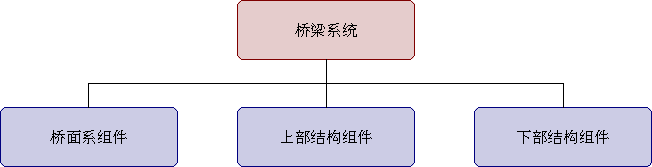
\includegraphics{bridge-system.pdf}
  % \caption{Bridge system composition}
  \caption{桥梁\gls*{system}的组成}
  \label{fig:bridge-system-composition}
\end{figure}

% As shown in \cref{fig:bridge-system-composition}, a bridge system is initially broken down into three main components: deck, superstructure and substructure. These are the primary categories or groupings of subsystems and elements within a bridge that define specific purpose and function.
如\cref{fig:bridge-system-composition} 所示,桥梁\gls*{system}最初分为三个主要部分:桥面系、上部结构和下部结构。 这些是定义特定目的和功能的桥梁\gls*{subsystem}和\gls*{element}的主要类别或分组。

% The deck component supports and receives live load and must provide a safe, smooth riding surface for traffic. It transfers live load and deck dead load to other components, which in most cases is to the superstructure. The superstructure component supports the deck and transmits loads across the span(s) to the bridge supports.
桥面系\gls*{component}支撑和承受活荷载,必须为交通提供安全、平稳的行驶表面。它将活载和桥面系恒载传递给其他\gls*{component},在大多数情况下是传递给上部结构。 上部结构\gls*{component}支撑桥面系并将各跨的荷载传递到桥梁支撑。

% The substructure component includes all elements that support the uperstructure. It transfers vertical and horizontal loads from the superstructure to the foundation material, such as soil or rock. At abutments, additional vertical and horizontal loads applied from the roadway embankment are also resisted.
下部结构\gls*{component}包括支持上部结构的所有\gls*{element}。 它将垂直和水平载荷从上部结构传递到基础材料(例如土壤或岩石)。 在桥台处,还可以抵抗来自车行道路堤的额外垂直和水平荷载。

% Often bridge systems are categorized or named by the superstructure type and material. This is discussed further in Section 2.2.3.
桥梁\gls*{system}通常按上部结构的类型和材料来分类或命名。这将在\cref{subsec:superstructure-componet}中进一步讨论。

% \subsection{Deck Component}
\subsection{桥面系\glsentrytext{component}}
\label{subsec:deck-component}
% \subsubsection{Deck Elements}
\subsubsection{桥面板\gls*{element}}

\begin{figure}
  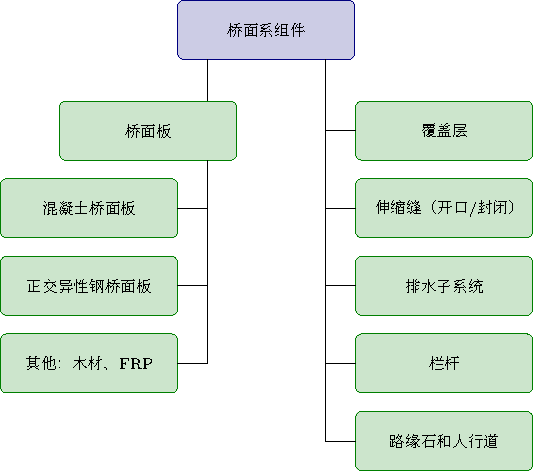
\includegraphics{component-deck.pdf}
  % \caption{Deck Componet}
  \caption{桥面系\gls*{component}}
  \label{fig:deck-component}
\end{figure}

% \cref{fig:deck-component} shows the various elements that make up the deck component, which includes the deck/slab element itself along with other related elements including overlays/wearing surfaces, expansion joints, drainage elements, railings, and curbs and sidewalks. There are various types of deck/slab elements, including concrete decks (either \acrfull{cip} or precast), steel/orthotropic decks (including open or concrete-filled steel grids), and other types including timber and FRP.
\cref{fig:deck-component} 显示了构成桥面系\gls*{component}的各种\gls*{element},其中包括桥面板\gls*{element}本身以及其他相关\gls*{element},包括覆盖层/耐磨表面、伸缩缝、排水系统\gls*{element}、栏杆和路缘石以及人行道。有多种类型的桥面板\gls*{element},包括混凝土桥面板(\acrfull{cip}或预制)、钢/正交各向异性桥面板(包括开放式或混凝土填充钢格栅)以及其他类型,包括木材和\acrfull{frp}。

% A detailed discussion of bridge decks and related service life issues is included in \cref{chp:bridge-decks}. Most decks are composite cast-in-place concrete types but other types composed of precast concrete panels (both partial depth and full depth) and posttensioning have been used, particularly with accelerated construction techniques. Steel deck types, including steel orthotropic decks, are also discussed in \cref{chp:bridge-decks}. A thorough look at materials used in bridge decks is provided in \cref{chp:materials}, and \cref{chp:expansion-devices} examines deck expansion devices and joints.
\cref{chp:bridge-decks}中包含对桥面板\gls*{servicelife}相关问题的详细讨论。 大多数桥面板是组合现浇混凝土类型,但也使用了由预制混凝土面板(部分深度和全深度)和后张法组成的其他类型,特别是当采用\acrfull{abc}技术时。\cref{chp:bridge-decks} 中还讨论了钢桥面板类型,包括钢正交各向异性桥面板。\cref{chp:materials} 中提供了对桥面系中使用的材料的全面了解,\cref{chp:expansion-devices}梳理了桥面板伸缩装置和接缝。

% \subsubsection{Bridge Deck Drainage}
\subsubsection{桥面系排水}
% The deck drainage subsystem includes inlets or scuppers, pipes and downspouts, and outlets. The main requirement of this subsystem is to remove rainfall-generated runoff from the bridge deck before it collects and spreads excessively in the gutter to encroach onto the traveled roadway. The deck drainage subsystem must be designed to deter flow and accompanying corrosive deicing chemicals from contacting vulnerable structural members. Proper maintenance of deck drainage elements is essential to avoid clogging and malfunction and such maintenance requirements must be considered in the design.
桥面系排水\gls*{subsystem}包括集水口或泄水孔、管道和落水管以及出水口。该\gls*{subsystem}的主要作用是将降雨产生的径流从桥面收集,并于其在排水沟中过度扩散并侵占行车道之前将其从桥面板中排除。 桥面系排水\gls*{subsystem}的设计必须能够阻止水流和伴随其的腐蚀性除冰盐等化学品接触脆弱的结构构件。恰当的维护桥面系排水\gls{element}对于避免堵塞和故障至关重要,并且在设计中必须考虑此类维护要求。

% Open expansion joint drainage includes collection troughs, pipes, and attachments below open expansion joints such as tooth or sliding plate dams to collect drainage, debris, and deicing chemicals that flow through the openings and protect adjacent structural elements. Again, proper maintenance is essential and must be factored into the design.
开放式伸缩缝排水包括收集槽、管道和开放式伸缩缝下方的附件,例如齿板或滑板,用于收集流经开口的排水、杂物和除冰化学品,并保护相邻的结构\gls*{element}。同样,恰当的维护是必不可少的,必须将其纳入设计中。

% \subsubsection{Bridge Railings}
\subsubsection{桥梁护栏}
% Materials used in bridge railing designs include metal, reinforced concrete, and various combinations. Crash testing requirements have been established by FHWA and AASHTO specifications to provide adequate strength depending on vehicle size and speed. Three general categories of bridge railings are typically considered: traffic railings, pedestrian or bicycle railings, and combination railings.
桥梁护栏设计中使用的材料包括金属、钢筋混凝土和各种组合材料。 \gls*{fhwa} 和 \gls*{aashto} 规范制定了碰撞测试要求,以根据车辆尺寸和速度提供足够的强度。通常考虑三种一般类别的桥梁护栏:车行护栏、行人或自行车护栏以及组合护栏。

% \begin{itemize}
  % \item Traffic railings are designed to contain and safely redirect vehicles.
  % \item Pedestrian or bicycle railings are generally located on the outside edge of a bridge sidewalk, and are designed to safely contain pedestrians or bicyclists. AASHTO specifications require certain heights and limit the opening sizes between members.
  % \item Combination railings are dual purpose railings designed to contain both vehicles and pedestrians or bicyclists, and are generally located at the outside edge of a bridge sidewalk. With this type of railing, there is usually no other barrier between the roadway and sidewalk.
% \end{itemize}
\begin{itemize}
  \item 交通栏杆旨在控制车辆并安全地重定向车辆。
  \item 行人或自行车栏杆通常位于桥人行道的外侧边缘,旨在安全地控制行人或骑自行车的人。 \acrshort*{aashto} 规范要求一定的高度并限制构件之间的开口尺寸。
  \item 组合栏杆是双重用途的栏杆,设计用于同时控制车辆和行人或骑自行车的人,通常位于桥梁人行道的外侧边缘。 使用这种类型的栏杆,车行道和人行道之间通常没有其他护栏。
\end{itemize}

% Bridge railings are often located in high splash zones and are often subject to harsh environments that effect steel element corrosion, concrete deterioration and reinforcing bar corrosion. Special protection is necessary for long-term service life of these elements.
桥梁栏杆通常位于高飞溅区域,并且经常受到影响钢\gls*{element}腐蚀、混凝土\gls*{deterioration}和钢筋腐蚀的恶劣环境。 这些\gls*{element}的长期\gls*{servicelife}需要特殊保护。

% Bridge rails are usually cast, following the deck casting. In these instances, special attention should be paid to the cold joint that will be created between deck and cast-in-place rail as it provides a natural path for ingress of moisture and causes corrosion of reinforcement.
桥梁栏杆通常在桥面板浇筑之后进行。 在这些情况下,应特别注意将在桥面板和现浇栏杆之间形成的冷接缝,因为它提供了水分进入的自然路径并导致钢筋腐蚀。

% \subsubsection{Curbs and sidewalks}
\subsubsection{路缘石和人行道}
% Curbs and sidewalks are affected similarly to deck slabs. Information relative to these elements is provided in \cref{chp:bridge-decks} on bridge decks and \cref{chp:materials} on materials.
路缘石和人行道所受到的影响与桥面板较为相似。有关这些\gls*{element}的信息将在\cref{chp:bridge-decks}\nameref{chp:bridge-decks}和\cref{chp:materials}\nameref{chp:materials}中提供。

% \subsection{Superstructure Component}
\subsection{上部结构\glsentrytext{component}}
\label{subsec:superstructure-componet}

% The superstructure component includes the structural subsystem and bearings. A detailed discussion of bearing elements is given in \cref{chp:bridge-bearings}.
上部结构部件包括结构\gls*{subsystem}和支座。\cref{chp:bridge-bearings}详细讨论了支座\gls*{element}。

\begin{figure}
  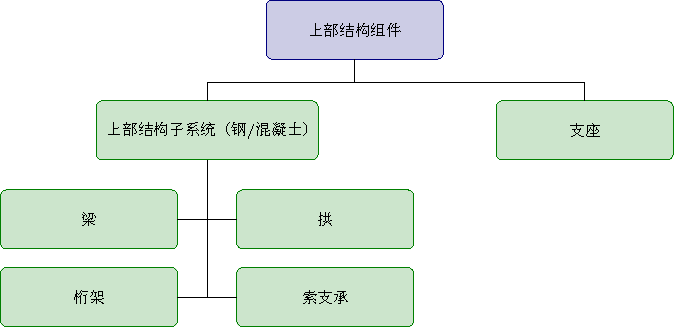
\includegraphics{component-superstructure.pdf}
  % \caption{Superstructure component}
  \caption{上部结构\gls*{component}}
  \label{fig:superstructure-component}
\end{figure}

% Superstructures are often categorized by:
上部结构通常按以下方式分类:
% \begin{itemize}
  % \item Material type. Steel or concrete are most commonly used.
  % \item Structure subsystem type. Girder subsystems are most often used for common-span lengths within the 300 feet limit. Longer spans typically use girders, trusses, arches or cable-supported types, depending on span length.
  % \item Superstructure continuity. Many older bridges were simple spans, while bridges that are more modern are fully continuous or continuous for live load. The continuous spans provide structural continuity that helps distribute traffic loads in case of excessive deterioration of some of the bridge elements. Structural continuity is especially important in instances of bridges with fracture critical elements.
  % \item Jointless Systems. Integral abutment construction is gaining popularity among many states. Integral pier construction is used only occasionally. Additional information on integral construction is provided in \cref{chp:jointless-bridge} on jointless bridges.
  % \item Modular Construction. Modular systems using prefabricated superstructure elements such as “topped girders” or preconstructed spans are becoming more popular in instances requiring accelerated construction. Durability of connection details is a concern for long-term service life of these systems. These types of connections are addressed in \cref{chp:jointless-bridge}on jointless bridges.
% \end{itemize}
\begin{itemize}
  \item 材料类型。最常用的是钢材或混凝土。
  \item 结构\gls*{subsystem}类型。 梁\gls*{subsystem}最常用于 \qty{90}{m} 以内的一般跨度。更大的跨度通常使用梁、桁架、拱或缆索支承类型,这具体取决于跨度长度。
  \item 上部结构的连续性。许多老的桥梁采用简支结构,而更现代的桥梁采用完全连续或对活荷载连续的结构。连续跨提供结构连续性,有助于在某些桥梁\gls*{element}过度\gls*{deterioration}的情况下重分配交通荷载。 结构连续性在具有断裂临界\gls*{element}的桥梁实例中尤为重要。
  \item 无缝系统。整体式桥台建设在许多州越来越受欢迎。整体式桥墩施工只是偶尔使用。 关于整体结构的更多信息在\cref{chp:jointless-bridge}\nameref{chp:jointless-bridge}中给出。
  \item 模块化建造。使用“预顶梁”或预制跨等预制上部结构\gls*{element}的模块化系统在需要\acrlong*{abc}的情况下变得越来越流行。 细部连接构造的耐久性是这些系统长期\gls*{servicelife}的一个问题。 这些类型的连接在\cref{chp:jointless-bridge}\nameref{chp:jointless-bridge}中进行了介绍。
\end{itemize}

% These categories are often combined in an overall classification of the superstructure, which is frequently used to define the entire bridge system.
这些类别通常结合在上部结构的总体分类中,经常用于定义整个桥梁\gls*{system}。

% Following is a brief discussion of the most common steel and concrete superstructure types.
以下是对最常见的钢和混凝土上部结构类型的简要讨论。

% \subsubsection{Steel Superstructures}
\subsubsection{上部钢结构}
% \paragraph{Steel Girder Superstructures} 
\paragraph{钢梁上部结构} 
% The most common steel bridge superstructures today are composite multi-girder subsystems that use either rolled beams, plate girders or tub girders. These systems can be single or multi span, and can be either straight or curved. Either of these can also be skewed. Rolled beam superstructures using W-shapes are used in shorter spans up to about 100 ft for simple spans and up to about 120 ft for continuous spans. Recently, deeper rolled shapes (44 in.) for bridge applications have become available. When combined with the simple for dead and continuous for live load concept, these W-shapes can be used for longer spans. Welded plate girders are usually used for spans over 120 ft \cite{nsba2008}. \cref{fig:typical-steel-girder-superstructures} shows typical steel I-girder and tub girder systems. Recently, folded plate beam sections have been developed for short span applications. See \ref{par:steel-modular-system} for steel modular systems.
当今最常见的钢桥上部结构是使用轧制梁、板梁或小箱梁的复合多梁子系统。这些系统可以是单跨或多跨,可以是直的也可以是弯的。这些类型中的任何一种也都可以斜交布置。使用 W 形的轧制梁上部结构用于较短的跨度,简支跨度可达约 \qty{30}{m},连续跨度可达约 \qty{35}{m}。最近,更深轧制形状(\qty{1.10}{m})也已经可以用于桥梁结构中。 当与\gls{sdcl}概念相结合时,这些 W 形可使用更大的跨度。焊接板梁通常用于 \qty{35}{m}以上的跨度\cite{nsba2008}。 \cref{fig:typical-steel-girder-superstructures} 显示了典型的钢工字梁和小箱梁系统。最近,折板梁截面已被开发用于短跨度应用,可参阅 \ref{par:steel-modular-system} 了解钢制模块化系统。

\begin{figure}
  \begin{minipage}{0.48\linewidth}\centering
    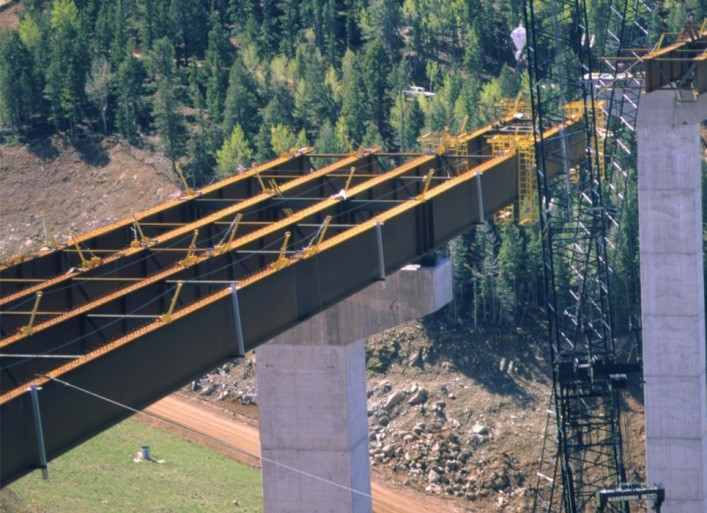
\includegraphics[height=5cm]{I-girder.jpg}
    % \subcaption{Deck I-girder system. (Courtesy HDR)}
    \subcaption{工字梁}
  \end{minipage}\hfill
  \begin{minipage}{0.48\linewidth}\centering
    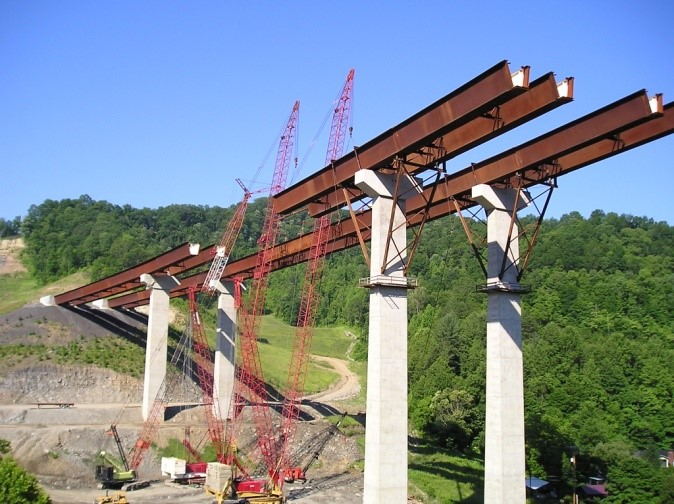
\includegraphics[height=5cm]{Tub-girder.jpg}
    % \subcaption{Tube girder system. (Courtesy Palmer Engineering)}
    \subcaption{小箱梁}
  \end{minipage}
  % \caption{Typical steel girder superstructures}
  \caption{典型钢梁上部结构}
  \label{fig:typical-steel-girder-superstructures}
\end{figure}

% Up until the 1970s, many bridges were designed with systems using two main deck girders, combined with transverse floor beams and longitudinal stringers. The perceived notion that two girder systems are not redundant led to a significant decrease in their use within the United States. However, two girder systems are very popular in Europe. Multi-girder bridges with inherent redundancy are currently preferred by many bridge owners (NSBA 2008). Use of high performance steels with greater fracture toughness, however, has led to re-evaluation of two-girder systems. Further, a memo dated June 20, 2012 by FHWA has paved the way to more use of two girder systems (FHWA 2012).
直到 20 世纪 70 年代,许多桥梁的设计系统都使用两个主纵梁,结合横梁和纵向小纵梁。 双主梁体系结构的冗余度不大,这样的观念导致它们在美国的使用很少,然而,双主梁体系在欧洲非常流行。在美国,具有固有冗余的多梁体系桥目前受到许多桥梁业主的青睐 \cite{nsba2008}。然而,在具有更高断裂韧性的高性能钢得到广泛应用后,人们对双主梁体系进行了重新评估。此外,\gls*{fhwa} 于 2012 年 6 月 20 日发布的一份备忘录为更多地使用双主梁体系铺平了道路\cite{fhwa2012a}。

% A variation to the typical multi-girder system is the girder-substringer system, which has been used as an economical concept for longer spans beyond approximately 275 ft. This system uses several heavy girders with wide girder spacing and rolled-beam stringers supported midway between the main girders by truss K-type cross frames.
典型的多梁体系的一个变体是主梁—子纵梁体系,它在被用于超过大约 \qty{83}{m} 的更大跨度时更为经济。该体系使用几个具有较大间距的重型主梁和中间支撑的轧制纵梁,主梁间采用桁架 K 型交叉框架作为横向联系。

% \paragraph{Continuity in Steel Systems}
\paragraph{钢结构体系中的连续性}

% For many years, bridges were designed as a series of simple spans with expansion joints at each pier because they were easy to design and construct. Leaking joints, however, became a leading cause of structural deterioration and the desire to eliminate joints became prevalent. Multi-span steel girder systems were also shown to be much more efficient when designed as continuous systems, making continuous design more commonplace.
多年来,桥梁被设计成一系列简支跨,每个桥墩都设有伸缩缝,因为它们易于设计和建造。 然而,当接缝缝的漏水成为结构\gls*{deterioration}的主要原因,消除接缝的愿望也就变得更普遍。当设计为连续系统时,多跨度钢梁体系也被证明效率更高,从而使连续设计更加普遍。

% Multi-span systems have typically been fully continuous for both dead load and live load, but new systems, typically with spans up to about 150 ft, have been introduced with a Simple for Dead Load and Continuous for Live Load (SDCL) concept. These systems combine the advantage of simple-span construction with the efficiency of live load continuity and the durability of not having joints that can ultimately leak.
多跨体系通常对于恒载和活载都是完全连续的,但是通常在跨度达到 \qty{45}{m} 的新体系中已经引入了\gls{sdcl}概念。 这些系统结合了简支跨建造的优势、活荷载连续性的效率以及没有最终可能漏水的接头的耐用性。

% Recently, extensive research studies have been carried out to develop practical details for SDCL steel bridge systems (Azizinamini et al. 2003, Azizinamini et al. 2005a, Azizinamini et al. 2005b; Azizinamini 2013; Lampe et al.2013; Farimani et al. 2013; Yakel and Azizinamini 2013; Javidi et al. 2013). These studies demonstrate that for the SDCL steel bridge system, continuity for live load can be provided using steel reinforcement placed over the pier, before casting deck; however, in order to provide continuity, various girder connection details have been used in practice. \cref{fig:steel-bridge-system-SDCL} shows two different details in use. Splice plates are sometimes used for top flange connections, which are in tension. The research studies previously referenced, however, do not recommend use of such detail. Bottom flanges in compression are typically butted with plates and wedges.
最近,在开发 \gls*{sdcl} 钢桥系统的实用细部构造方面已经开展了广泛的研究 \cite{azizinamini2003t,azizinamini2005d1,azizinamini2005d2,azizinamini2014s,lampe2013d,farimani2014n,yakel2014f,javidi2013e} 。这些研究表明,对于 \gls*{sdcl} 钢桥系统,在浇筑桥面之前,可以使用在墩顶设置的钢筋来提供活荷载的连续性;然而,为了提供连续性,在实践中使用了各种梁连接构造。\cref{fig:steel-bridge-system-SDCL} 显示了两个不同的细部构造:顶部受拉翼缘板有时用拼接板连接,然而,先前引用的研究不建议使用此类构造;底部受压的翼缘板通常采用板和楔子顶紧。

% The disadvantage of the continuity detail with the top flange splice is that the bolts for connecting the top plate have to be tightened after casting the deck. This creates additional construction sequencing with a separate closure pour over the pier.
顶部受拉翼缘板拼接的连续构造的缺点是在浇铸桥面板后必须拧紧用于连接顶板的螺栓。 这会创建额外的施工顺序,并在桥墩上单独浇筑。

\begin{figure}
  \begin{minipage}{0.48\linewidth}\centering
    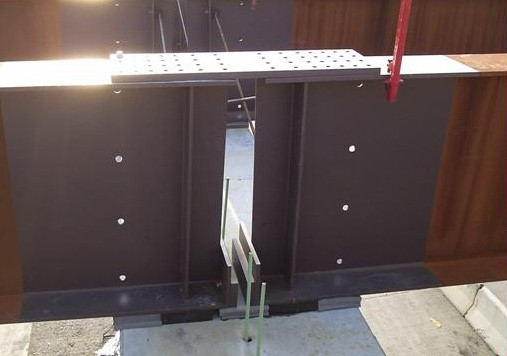
\includegraphics[height=5cm]{cont-with-top-flange-splice.jpg}
    \subcaption{顶部翼缘板带有拼接的桥面连续}
  \end{minipage}\hfill
  \begin{minipage}{0.48\linewidth}\centering
    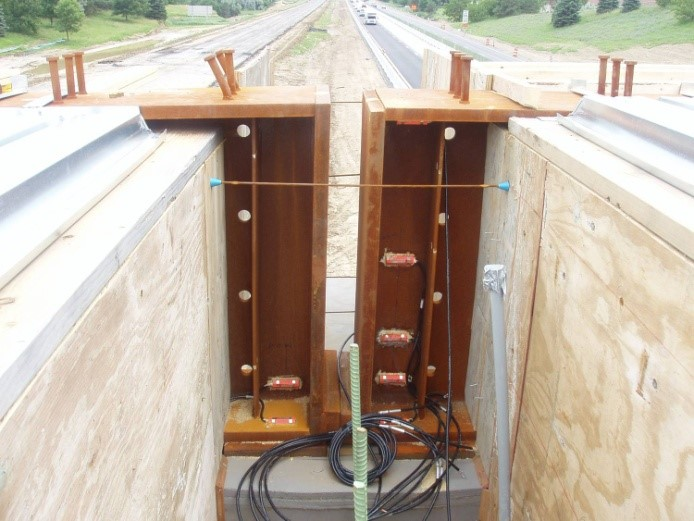
\includegraphics[height=5cm]{cont-without-top-flange-splice.jpg}
    \subcaption{顶部翼缘板不带拼接的桥面连续}
  \end{minipage}
  \caption{\acrshort*{sdcl}概念的钢桥}\label{fig:steel-bridge-system-SDCL}
\end{figure}

% \paragraph{Long-Span Superstructures}
\paragraph{大跨度上部结构}

% \cref{fig:long-span-steel-bridge-superstructures} shows examples of long-span girder, truss, arch, and cable-stayed bridge systems. Steel plate girder systems have been used for spans up to approximately 500 ft. Spans up to 400 ft have been designed economically with parallel flanges. Variable-depth haunched girders have been used in the 350-ft to 500-ft range. Use of highperformance steel (HPS 70W) has shown economy for plate girder and tub girder systems in most span ranges over 150 ft, particularly in hybrid combinations. Studies have shown that hybrid configurations using conventional grade 50W steel in webs and HPS 70W steel in top and bottom flanges in negative moment regions and bottom flanges in positive moment regions are typically the most economical (Horton et al. 2002). Top flanges in positive moment regions are affected by composite action with the deck and cannot realize enough benefit from the use of higherstrength steel to be economical, except for longer spans. Use of HPS 70W steel in long-span negative moment ranges can also permit economical parallel flange design without expensive haunches. Trusses, arches, cable-stayed, and suspension systems have also been used for longer-span applications, typically over 500 feet. For spans up to 300 feet, deck girder systems are the most applicable.
\cref{fig:long-span-steel-bridge-superstructures} 显示了大跨度梁、桁架、拱和斜拉桥体系的示例。钢板梁体系已用于高达约 \qty{150}{m} 的跨度。\qty{120}{m} 的跨度已被设计为具有平行翼缘板的经济型。 在 \qtyrange{105}{150}{m} 的范围内使用了变高度的加腋梁。在超过 \qty{45}{m} 的大多数跨度范围内,特别是在不同钢种的混合配置中,高性能钢(HPS 70W)的使用已经显示出钢板梁和钢小箱梁系统的经济性。研究表明,在腹板中使用传统等级 50W 钢,在负弯矩区域的顶底部翼缘板和正弯矩区域底部翼缘板中使用 HPS 70W 钢,这种混合配置通常是最经济的 \cite{horton2003h}。正弯矩区域的顶部翼缘受到与桥面板的联合作用的影响,并且不能从使用高强度钢中获得足够的好处以达到经济的目的,除非是更长的跨度。在大跨度负弯矩范围内使用 HPS 70W 钢还可以实现经济的平行翼缘板设计,而无需昂贵的腰部。 桁架、拱、斜拉索和悬吊系统也已用于较长跨度的应用,通常超过 \qty{150}{m}。 对于 \qty{90}{m} 以内的跨度,钢板梁系统是最适用的。

\begin{figure}
  \begin{minipage}{0.48\linewidth}\centering
    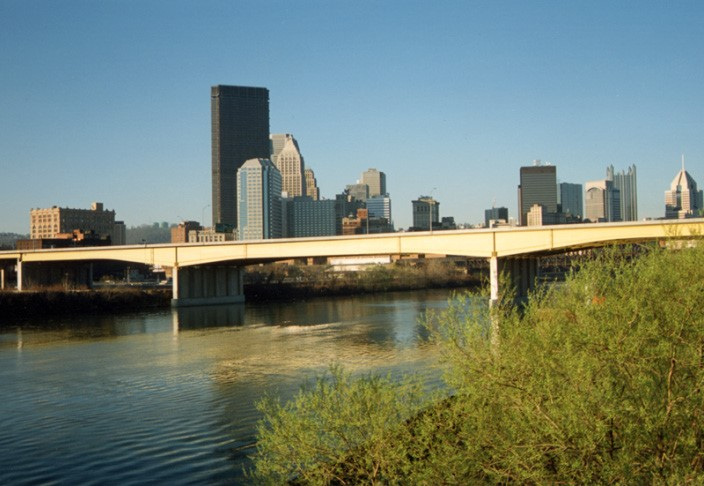
\includegraphics[height=5cm]{long-span-plate-girder.jpg}
    \subcaption{大跨度板梁}
  \end{minipage}\hfill
  \begin{minipage}{0.48\linewidth}\centering
    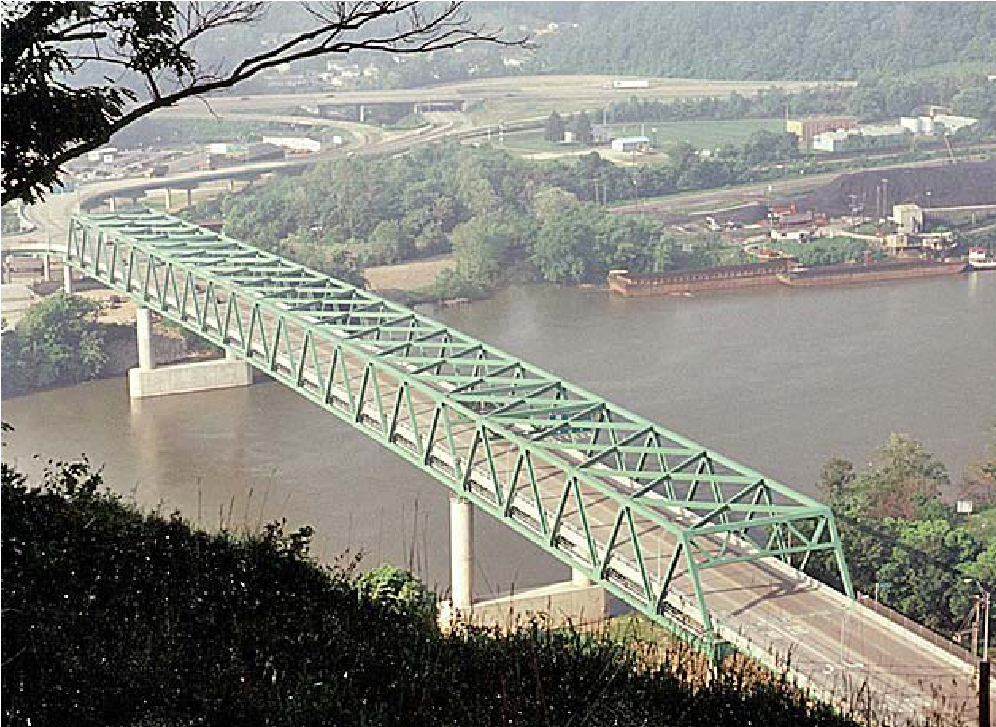
\includegraphics[height=5cm]{continuous-truss.png}
    \subcaption{连续桁架}
  \end{minipage}
  \begin{minipage}{0.46\linewidth}\centering
    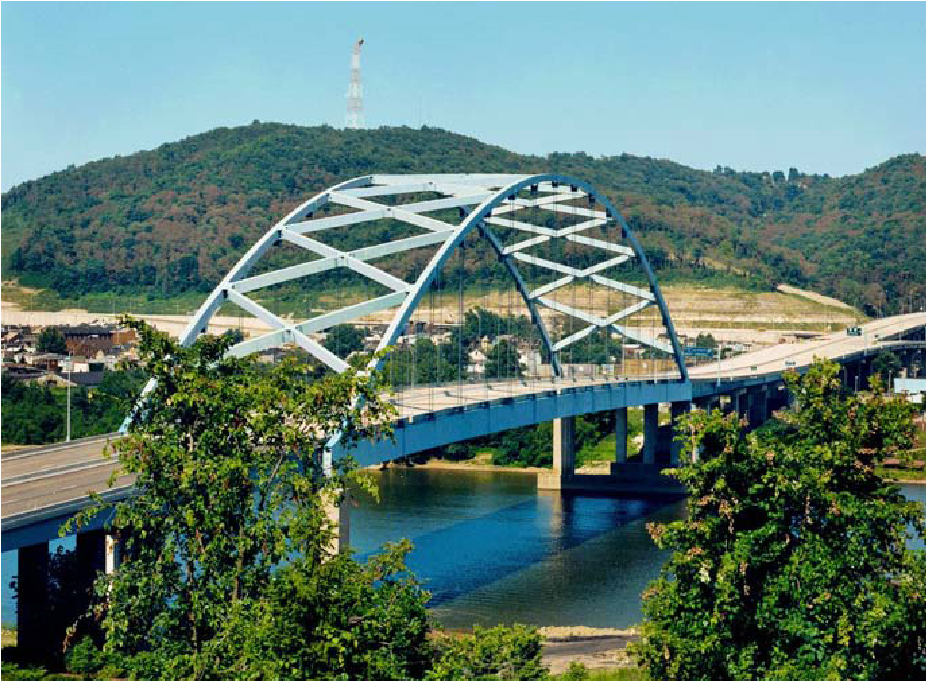
\includegraphics[height=5cm]{tied-arch.png}
    \subcaption{系杆拱}
  \end{minipage}\hfill
  \begin{minipage}{0.52\linewidth}\centering
    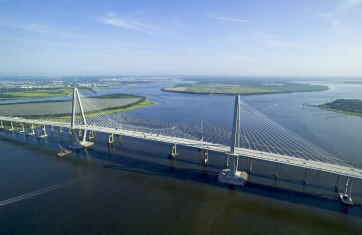
\includegraphics[height=5cm]{cable-supported.jpg}
    \subcaption{索支承桥梁}
  \end{minipage}
  % \caption{Long-span steel bridge superstructures. (All Figures Courtesy HDR)}
  \caption{大跨度钢桥上部结构}
  \label{fig:long-span-steel-bridge-superstructures}
\end{figure}

% Long-span structures can have special needs for addressing long-term service life relating to unique details, inspection, and maintenance. Access for inspection and maintenance can require elaborate systems of inspection walkways and access ladders, particularly for access to fracture-critical members. Older trusses typically require heavy maintenance because of large surface area to weight ratio, and riveted, built-up members with lacing bars subject to pack-out and other surface corrosion. Truss joint details typically have moisture and debris traps that initiate corrosion, while newer trusses have cleaner surface details that are more easily painted and maintained.
大跨度结构在解决与独特细节、检查和维护相关的长期使用寿命方面可能有特殊需求。 检查和维护通道可能需要精心设计的检查走道和通道梯系统,特别是对于断裂关键部件的通道。较旧的桁架通常需要大量维护,因为它的表面积与重量比很大,并且带有拉筋的铆接组合构件容易被压裂和其他表面腐蚀。桁架接头细节通常有湿气和杂物陷阱,会引发腐蚀,而较新的桁架有更清洁的表面细节,更容易涂漆和维护。

% Through structures are subject to splash zone wetting environments for all structural elements near roadway edges. This needs to be considered in a corrosion protection and maintenance plan. Long-span bridges have large thermal movement requirements that result in large expansion joints. This requires even additional attention to joint maintenance to prevent deck drainage from spilling through. Heavy loads and large thermal movements also require special bearing designs. Navigation channel crossings are subject to vessel collision and need to be protected.
对于靠近道路边缘的所有结构\gls*{element},贯通结构都受到飞溅区润湿环境的影响。这需要在腐蚀保护和维护计划中加以考虑。大跨度桥梁具有较大的温度作用变形要求,因此会需要较大的伸缩缝。 这甚至需要额外注意接头维护,以防止桥面板排水系统溢出。 重载荷和大的温度作用变形也需要特殊的支座设计。 航道交叉口容易受到船只碰撞,需要加以保护。

% \paragraph{Steel Modular Systems}
\paragraph{钢结构模块化系统}
\label{par:steel-modular-system}

% New steel systems that provide for accelerated construction include modular construction with pre-topped deck. Modular orthotropic deck systems are also a consideration. These modular systems require special attention to both transverse and longitudinal connection details for achieving long-term durability.
提供快速建造的新钢系统包括带有预顶板的模块化结构。 模块化正交各向异性桥面板系统也是一个考虑因素。 这些模块化系统需要特别注意横向和纵向连接构造,以实现长期耐用性。

% Pre-top modular bridge systems are best suited for accelerated bridge construction applications. In these systems, several units consisting of pre-topped steel or concrete girders are placed side by side and joined together using longitudinal closure pours. The service life of these pre-topped modular systems is significantly influenced by service life of longitudinal closure pour. Pre-topped steel modular systems present two major advantages:
预顶模块化桥梁系统最适合\acrlong*{abc}应用。 在这些系统中,几个由预顶钢或混凝土梁组成的单元并排放置,并使用纵向闭合浇注连接在一起。 这些预先加盖的模块化系统的{使用寿命}受纵向封闭浇注的{使用寿命}的显着影响。 预盖钢模块化系统具有两大优势:

% \begin{enumerate}
%   \item The use of steel girders significantly reduces the creep and shrinkage deflections.
%   \item Pre-topped steel modular units weigh less.
% \end{enumerate}
\begin{enumerate}
  \item 钢梁的使用显着降低了蠕变和收缩挠度。
  \item 预顶的钢结构模块化单元重量更轻。
\end{enumerate}

% The Folded Plate Bridge System is a new modular system that offers an economical solution for many short-span bridge applications. The system consists of a series of standard shapes that are built by bending flat plates into inverted tub sections using a press break, as shown in \cref{fig:making-of-folded-plate-girder-using-break-press}.
折叠板桥系统是一种新型模块化系统,可为许多短跨度桥梁应用提供经济的解决方案。 该系统由一系列标准形状组成,这些标准形状是通过使用压力折断将平板弯曲成倒置的桶形部分而构建的,如 \cref{fig:making-of-folded-plate-girder-using-break-press} 所示。

\begin{figure}
  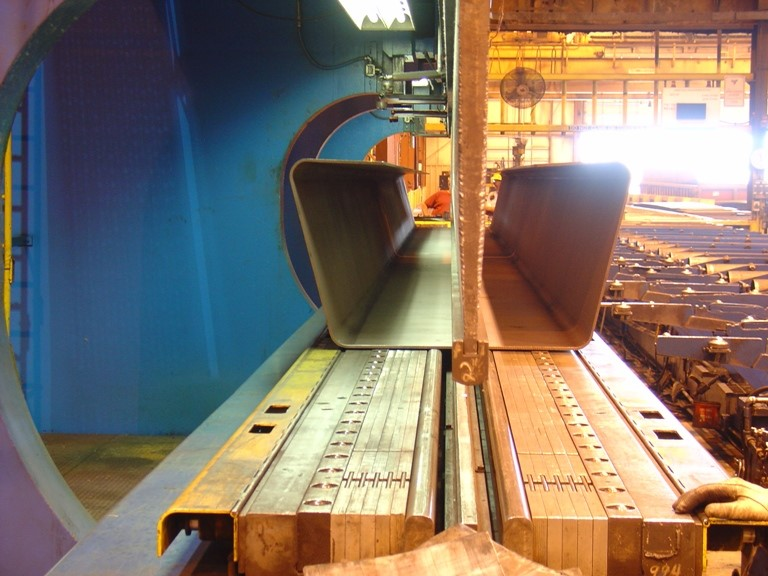
\includegraphics[width=0.7\linewidth]{folded-plate.jpg}
  % \caption{Making of folded plate girder using break press. (Courtesy UNL)}
  \caption{使用断裂压力机制作折叠板梁(由 \acrshort{unl} 提供)}
  \label{fig:making-of-folded-plate-girder-using-break-press}
\end{figure}

% The maximum span length for this system is currently limited to about 60 feet, reflecting the longest press breaks available in the industry.
该系统的最大跨度长度目前限制在 60 英尺左右,反映了行业中可用的最长压力中断。

% The process of bending the girder can take less than an hour. Geometrical variations are obtained simply by changing the bend locations. Varying the depth of the web and the width of the top and bottom flanges allow the folded plate girders to accommodate different span length requirements.
弯曲大梁的过程可能需要不到一个小时。 只需改变弯曲位置即可获得几何变化。 改变腹板的深度以及顶部和底部翼缘的宽度允许折叠板梁适应不同的跨度长度要求。

% One of the advantages of the Folded Plate Bridge System is its promise for rapid delivery. All folded plate girders are fabricated using either 0.375- or 0.5-in. thick plate. The ability to stock standard plate sizes means the girders can be produced and delivered quickly.
折叠板桥系统的优势之一是它对快速交付的承诺。 所有折叠板梁均使用 0.375 或 0.5 英寸制造。 厚板。 库存标准板尺寸的能力意味着可以快速生产和交付大梁。

% The Folded Plate Bridge System can be constructed using conventional construction techniques as well as using principles of Accelerated Bridge Construction. In the case of conventional construction procedures, readily available construction equipment can be used to build the formwork for casting the concrete deck, as shown in \cref{fig:deck-forming-conventional}.
折叠板桥系统可以使用传统的施工技术以及\acrlong{abc}的原理来建造。 在传统施工程序的情况下,现成的施工设备可用于建造用于浇注混凝土甲板的模板,如 \cref{fig:deck-forming-conventional} 所示。

\begin{figure}
    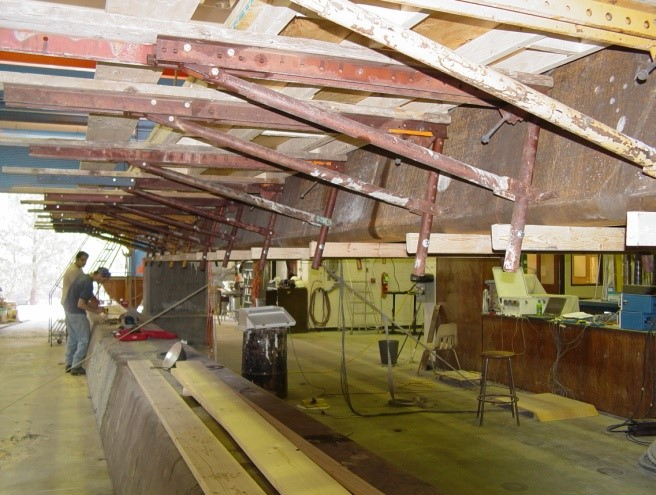
\includegraphics[height=5.5cm]{deck-forming1.jpg}\hfill
    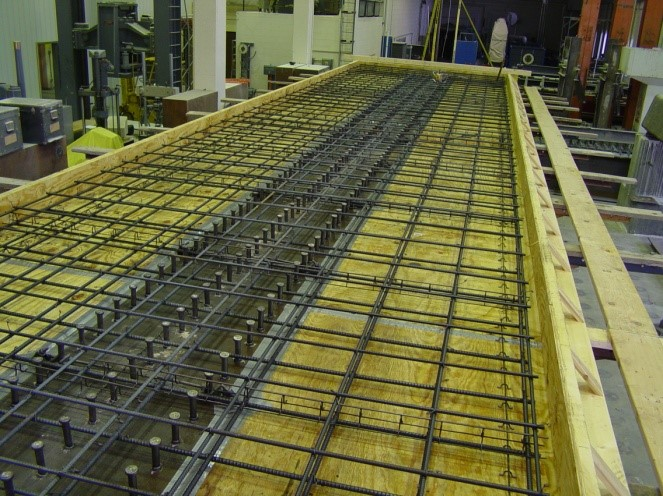
\includegraphics[height=5.5cm]{deck-forming2.jpg}
  % \caption{Deck forming using conventional approach. (Courtesy UNL)}
  \caption{使用传统方法施工桥面板(由 \acrshort{unl} 提供)}
  \label{fig:deck-forming-conventional}
\end{figure}

% Recently, the trend within the bridge construction industry has been toward reducing construction activities on the bridge site and eliminating the interruption to traffic. Therefore, an alternate and perhaps better approach when using the Folded Plate Girder System to construct short-span bridges is to use prefabricated elements.
近来,桥梁建设行业的趋势是减少桥梁现场的施工活动并消除交通中断。 因此,使用折叠板梁系统建造短跨度桥梁时,另一种可能更好的方法是使用预制构件。

% In one scenario, the tributary width of concrete deck for each folded plate girder is cast on the girder prior to shipping to the site. In this case, each prefabricated girder unit is a folded plate girder with a precast deck as shown in \cref{fig:precast-folded-plate-girder-unit}. The steel girder can be supported at the ends, or continuously supported along the length during casting, in which case all dead loads are carried by the composite section, thereby reducing deflections.
在一种情况下,每个折叠板梁的混凝土桥面板的支流宽度在运输到现场之前浇铸在梁上。 在这种情况下,每个预制梁单元都是带有预制桥面板的折叠板梁,如 \cref{fig:precast-folded-plate-girder-unit} 所示。 钢梁可以在端部支撑,也可以在浇铸过程中沿长度连续支撑,在这种情况下,所有恒载均由复合截面承载,从而减少挠度。

\begin{figure}
  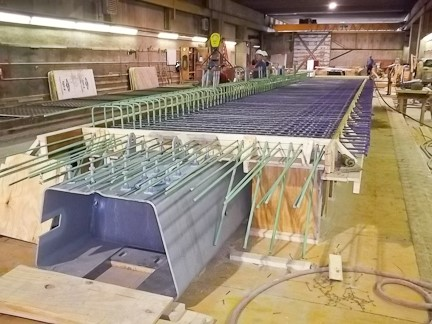
\includegraphics[height=5.5cm]{precast-unit1.jpg}\hfill
  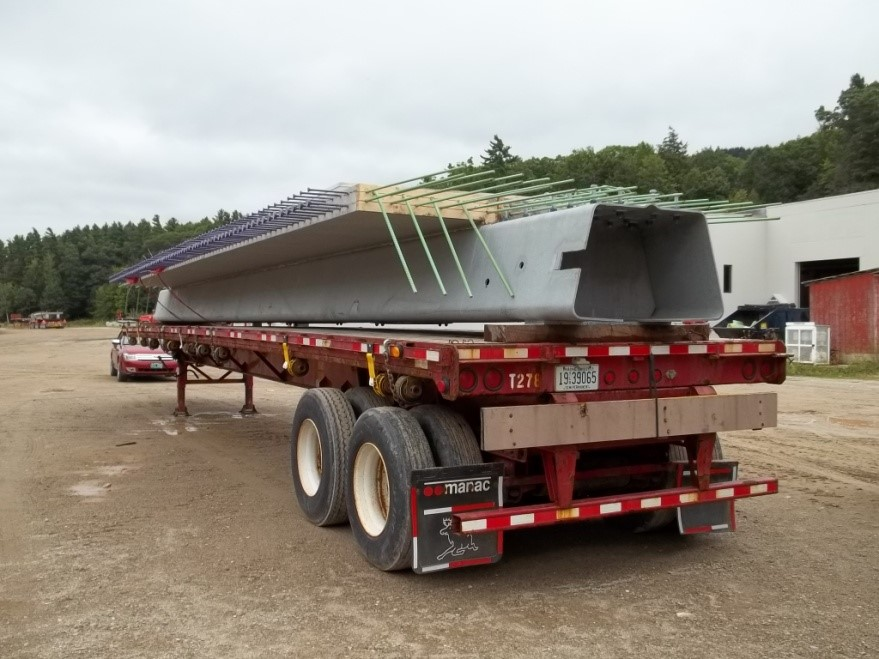
\includegraphics[height=5.5cm]{precast-unit2.jpg}
  % \caption{Precast folded plate girder unit. (Courtesy Massachusetts DOT)}
  \caption{预制折板梁单元(由马萨诸塞州\acrlong*{dot}提供)}
  \label{fig:precast-folded-plate-girder-unit}
\end{figure}

% A typical two-lane county-type bridge will require three or four prefabricated folded plate girder units placed side by side and connected longitudinally at the deck, as shown in \cref{fig:folded-plate-girder-system}. The connection between the units can be accomplished using a number of methods. A 40-ft-long folded plate girder with precast deck weighs about 24,000 pounds, allowing use of a relatively lightweight crane on the construction site.
一座典型的双车道县级桥梁将需要三个或四个预制折叠板梁单元并排放置并在桥面板上纵向连接,如\cref{fig:folded-plate-girder-system} 所示。单元之间的连接可以使用多种方法来完成。一个 \qty{12}{m} 长的带预制桥面板的折叠板梁重约 \qty{10.9}{\tonne},允许在施工现场使用相对轻便的起重机。

\begin{figure}
  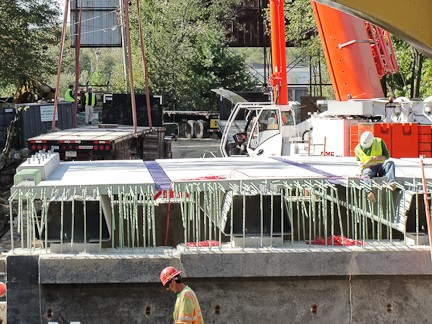
\includegraphics[height=5.5cm]{folded-plate-girder1.jpg}\hfill
  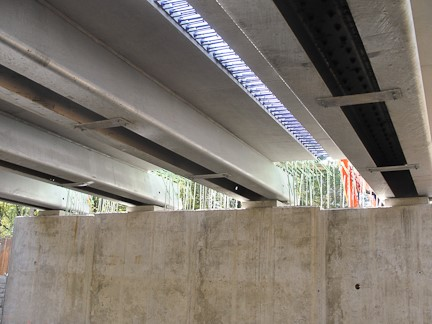
\includegraphics[height=5.5cm]{folded-plate-girder2.jpg}
  % \caption{Folded plate girder system. (Courtesy Massachusetts DOT)}
  \caption{折板梁系统(由马萨诸塞州\acrlong*{dot}提供)}
  \label{fig:folded-plate-girder-system}
\end{figure}

% \subsubsection{Concrete Bridge Superstructures}
\subsubsection{混凝土桥梁上部结构}

% There are several commonly used reinforced concrete bridge systems in the United States. The type of system implemented at a particular site is generally dictated by economics and the system's ability to accommodate the required span, or geometric requirements such as curvature.
美国有几种常用的钢筋混凝土桥梁体系。 在特定地点实施的系统类型通常由经济性和系统适应所需跨度或几何要求(如曲率)的能力决定。

% The most commonly used concrete bridge superstructures are:
最常用的混凝土桥梁上部结构有:

% \begin{itemize}
%   \item Cast-in-place concrete slabs;
%   \item Precast concrete box beams including both spread and adjacent box beams;
%   \item Precast concrete I-girders including standard I-girders, bulb-tee girders, and U-beams;
%   \item Precast concrete spliced girders, including spliced I-girders, U-beams, and box girders;
%   \item Cast-in-place posttensioned box girders;
%   \item Segmental posttensioned concrete box girders, including both precast or cast-in-place;
%   \item Concrete arches; and
%   \item Modular pre-topped concrete girder units, which are typically used for accelerated bridge construction.
% \end{itemize}
\begin{itemize}
  \item 现浇混凝土板桥;
  \item Precast concrete box beams including both spread and adjacent box beams;
  \item Precast concrete I-girders including standard I-girders, bulb-tee girders, and U-beams;
  \item Precast concrete spliced girders, including spliced I-girders, U-beams, and box girders;
  \item Cast-in-place posttensioned box girders;
  \item Segmental posttensioned concrete box girders, including both precast or cast-in-place;
  \item Concrete arches; and
  \item Modular pre-topped concrete girder units, which are typically used for accelerated bridge construction.
\end{itemize}

% \paragraph{Cast-in-Place (CIP) Concrete Slabs}
\paragraph{现浇混凝土板桥}

Full-depth, cast-in-place concrete slab superstructures consist of a concrete slab spanning between substructure units without the aid of supporting stringers, as shown in \cref{fig:short-span-concrete-bridge-applications}. Concrete slab bridges commonly span less than 50 feet and are typically used over minor water crossings. This bridge system was traditionally constructed as a series of simple spans, but in recent years, the use of continuous spans has gained favor, eliminating the joints over the substructure units. This system is commonly reinforced conventionally, but can also be posttensioned to increase the span length range. The haunched posttensioned concrete slab system used in Kansas can span up to about 100 feet. Many states, especially in the Midwest, own many older concrete slab bridges, mainly constructed in 1930s, that have shown a very good performance history. When rated, these older concrete slab bridges usually demand posting. However, research results indicate that older concrete slab bridges possess reserve capacity significantly more than that indicated by routine rating calculations (Azizinamini et al. 1994a, 1994b). The main reason for such high capacity of older concrete slab bridges is the higher yield strength of reinforcement used versus the assumed value in rating calculations. This higher capacity of existing older concrete slab bridges coupled with their good performance record can be advantageous when developing maintenance plans.

\begin{figure}
  \begin{minipage}{0.49\linewidth}\centering
    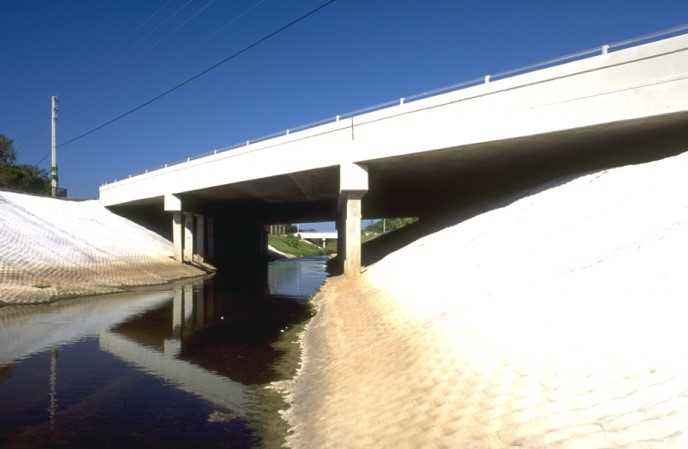
\includegraphics[height=4.8cm]{flat-slab.jpg}
    \subcaption{现浇混凝土平板桥}
  \end{minipage}\hfill
  \begin{minipage}{0.49\linewidth}\centering
    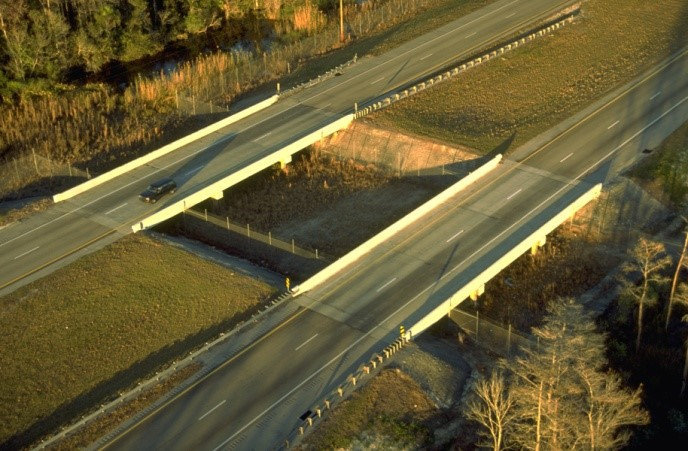
\includegraphics[height=4.8cm]{transv-post-prestress.jpg}
    \subcaption{横向后张法预应力板}
  \end{minipage}
  % \caption{Short-span concrete bridge applications. (Courtesy Atkins North America, Inc.)}
  \caption{小跨径混凝土桥梁的应用}
  \label{fig:short-span-concrete-bridge-applications}
\end{figure}

\paragraph{Precast Concrete Box Beams}

This type of superstructure consists of adjacent precast concrete box beams with non-composite deck, adjacent box beams with composite cast-in-place (CIP) concrete deck, and spread box beams with composite CIP concrete deck. Shallower precast solid and voided rectangular slabs also fall into this category. Precast concrete box beams are typically plant manufactured standard AASHTO-PCI sections that range in depth from 27 in. to 42 in. and are available in 36-in. or 48-in. widths. These precast girders are plant-produced, which generally results in high quality products.

Precast adjacent box beam bridges are the most prevalent box girder system for short and medium-span bridges, typically 20 to 127 feet, especially on secondary roadways. These bridges consist of multiple precast concrete box beams that are butted against each other to form the bridge deck and superstructure. Their advantage is that they eliminate the need for forming when using a composite CIP deck, or can be used directly with a bituminous overlay in the non-composite state. Adjacent box beams are generally connected using partial or full-depth grouted shear keys along the sides of each box. Transverse ties are usually used in addition to the grouted shear keys and may vary from a limited number of threaded rods to several posttensioned tendons. In some cases, no topping is applied to the structure while in other cases a non-composite topping or a composite structural slab is added. Problems have been encountered with adjacent non-composite box beam superstructures and are further discussed in Section 2.3.3.2.2.

\paragraph{Precast Concrete Girders}

Precast concrete I-girders with composite cast-in-place deck are commonly used concrete bridge superstructures in the 50- to 150-ft-plus span range. These girders are made of high-performance, plant-produced materials and are generally very durable and result in high quality products. In a bridge system consisting of I-girders with composite CIP slabs, commonly referred to as beam-slab bridges (see \cref{fig:concrete-I-girder-with-composite-deck}), the longitudinal stringers are often prestressed concrete I-girders using one of six standard AASHTO-PCI sections, Types I through VI, which vary in depth from 28 to 54 in. In addition, newer standard AASHTO-PCI bulb-tee (BT) shapes are used in 54-, 63-, and 72- in. depths. These standard I and BT shapes accommodate various span requirements up to about 170 ft.

Bulb-tee shapes were developed to provide increased efficiency over original I shapes. They have wide top flanges similar to Type V and VI girders that increase stability for handling and shipping and reduce deck forming. However, bulb-tees also have thinner top flanges, webs and bottom flanges that reduce weight, and have other flange geometric and proportioning modifications that optimize the sections. A number of states including Washington, Colorado, Florida and Nebraska have developed special bulb-tee shapes, modifying the standard AASHTO-PCI BT shapes, to accommodate local needs and practice.

\begin{figure}
  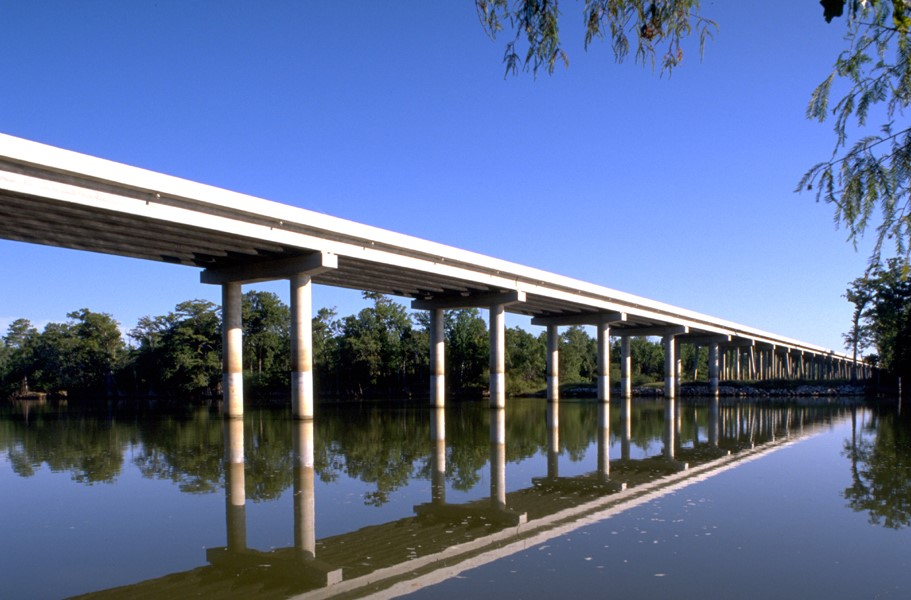
\includegraphics[width=0.8\linewidth]{concrete-I-girder-with-composite-deck.jpg}
  % \caption{Prestressed concrete I-girder bridge with composite concrete deck. (Courtesy Atkins North America, Inc.)}
  \caption{带复合混凝土桥面板的预应力混凝土工字梁桥}
  \label{fig:concrete-I-girder-with-composite-deck}
\end{figure}

A noteworthy I-girder advancement is the NU I-girder, which was developed by the University of Nebraska (UNL) in cooperation with the Nebraska Department of Roads, and has a series of eight standard shapes with depths ranging from 29.5 to 94.5 in. (Geren and Tadros 1994; Hanna et al. 2010). The NU girders have several section efficiency enhancements such as wide and thick bottom flanges that enable increased strand capacity for simple spans and provide increased negative moment capacity for continuous spans. The wide bottom flanges also provide increased stability in shipping and handling. Curved fillets in top and bottom flanges reduce stress concentration and aid the flow of concrete during fabrication. With the increased section efficiencies, these girders have been used for spans greater than \qty{60}{m} (see \cref{fig:nu-i-girder}).

\begin{figure}
  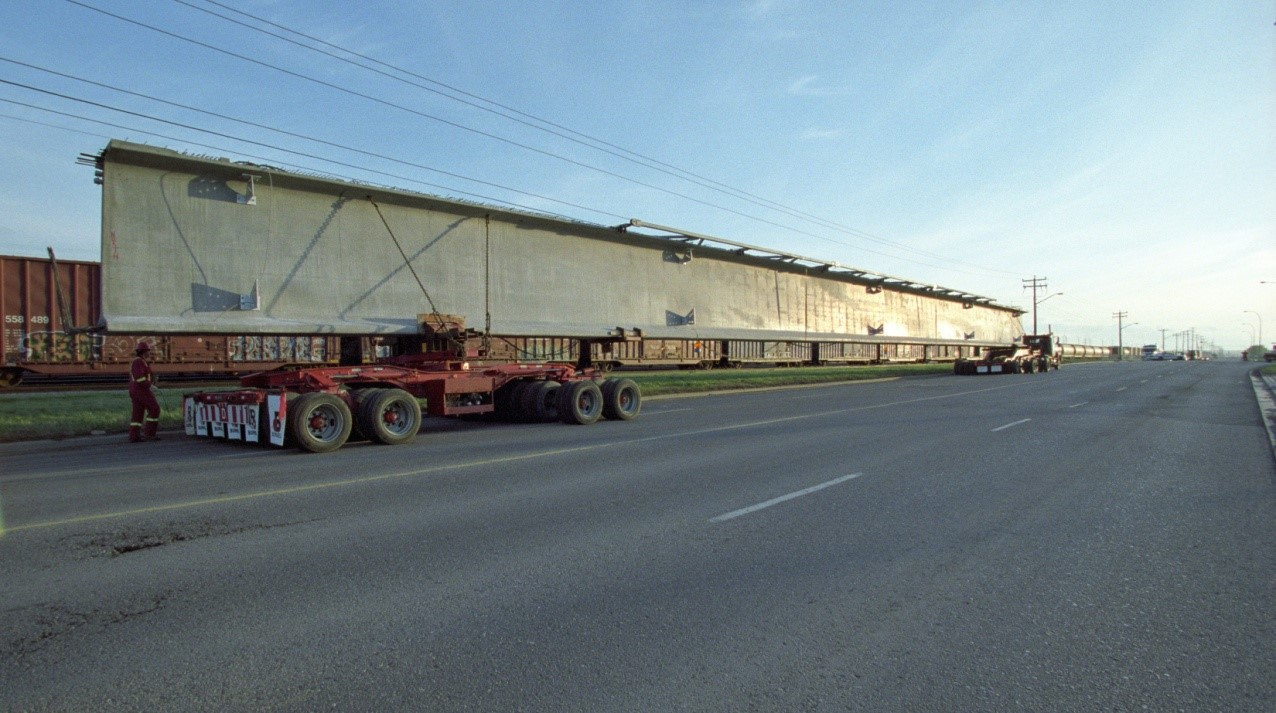
\includegraphics[width=0.9\linewidth]{nu-i-girder.jpg}
  % \caption{A 9-ft x 3-in. deep, 213-ft-long, 130-ton NU I-girder being shipped. (Courtesy of Con-Force Structures, a division of Armtec Limited Partnership, Calgary, Alberta, Canada)}
  \caption{长 \qty{65}{m}、高 \qty{2.8}{m}、重 \qty{130}{t} 的 NU I 型梁正在装运。}
  \label{fig:nu-i-girder}
\end{figure}

In many instances, precast concrete I-girders are erected as simple spans and then connected over the piers to form continuous for live load systems that eliminate deck joints.

A newer alternative to concrete I-girders is the U-beam, or concrete tub girder, concept, first developed in Texas
and now used in other states including Florida and Washington State, that provides economic and aesthetic spread
beam systems. The Texas U54 beam is 54-in. deep, similar to an AASHTO Type IV beam, and can span up to about
140 feet (Ralls et al. 1993). The Florida U-beams have four depths ranging from 48 in. to 72 in., and can be used in
spans ranging from about 100 ft to 160 ft (FDOT 2012). Washington State (WSDOT) U-beams are similar and have
four depths varying from 54 in. to 72 in., and bottom flanges that are either 4-ft or 5-ft wide. Similar to Florida, these beams can accommodate span lengths up to 160 ft. With a composite concrete deck, U- beams form a trapezoidal
box shape, similar to steel tub girders. These beams are typically designed to act as simple spans under both dead
load and live load, even when the deck is placed continuous across intermediate supports. As with I-girders, these
beams are plant produced and result in high quality products.

\paragraph{Precast Concrete Spliced Girders}
Spliced girders are precast concrete girders fabricated in several segments that are then assembled
longitudinally, typically using posttensioning, into a single simple-span or continuous girder for the final bridge
structure. They have been used to extend the span lengths of regular short- to medium-span precast concrete girders
and are designed to utilize the economy and high quality of plant-produced precast girders for longer span
applications. The length and weight of typical precast girders prevents them from being effectively used on spans
greater than about 150-feet due to the limitations of transportation equipment and available cranes. However, with
spliced girders, precast girder segments with manageable weights and lengths are transported to the construction site
and then joined together. This can either be done by splicing girder segments on the ground and erected them into
their final position, or by placing girder segments on temporary supports and then splicing them in their final
position. Spliced girders have been used for simple spans up to about 220 ft, and for continuous spans up to about
320 ft, and have been found to provide an economical concrete superstructure type in span ranges between that of
conventional precast girders and segmental box girders. \cref{fig:spliced-i-girder} shows a typical spliced girder span under
construction using temporary supports.

\begin{figure}
  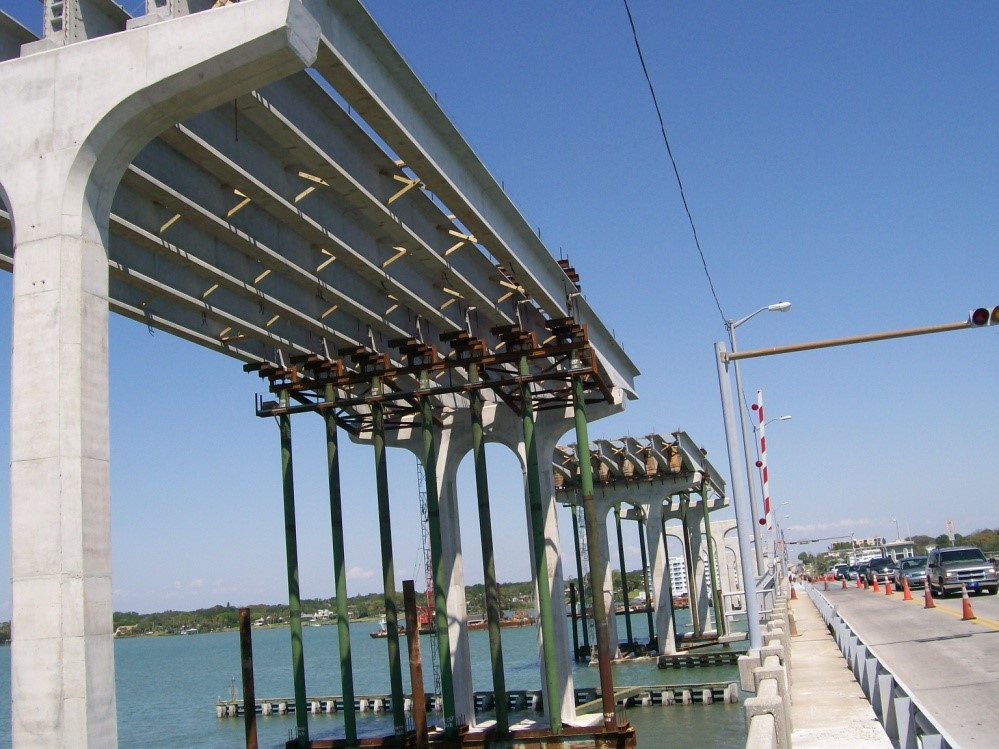
\includegraphics[width=0.65\linewidth]{spliced-i-girder.jpg}
  \caption{Spliced I-girder construction. (Courtesy HDR)}\label{fig:spliced-i-girder}
\end{figure}


Spliced girders are typically used on relatively straight alignments; however, in recent years they have also been
used for curved alignments in Nebraska and Colorado. \cref{fig:spliced-concrete-curved-box} shows a spliced-box girder bridge recently built
in Denver, Colorado.

\begin{figure}
  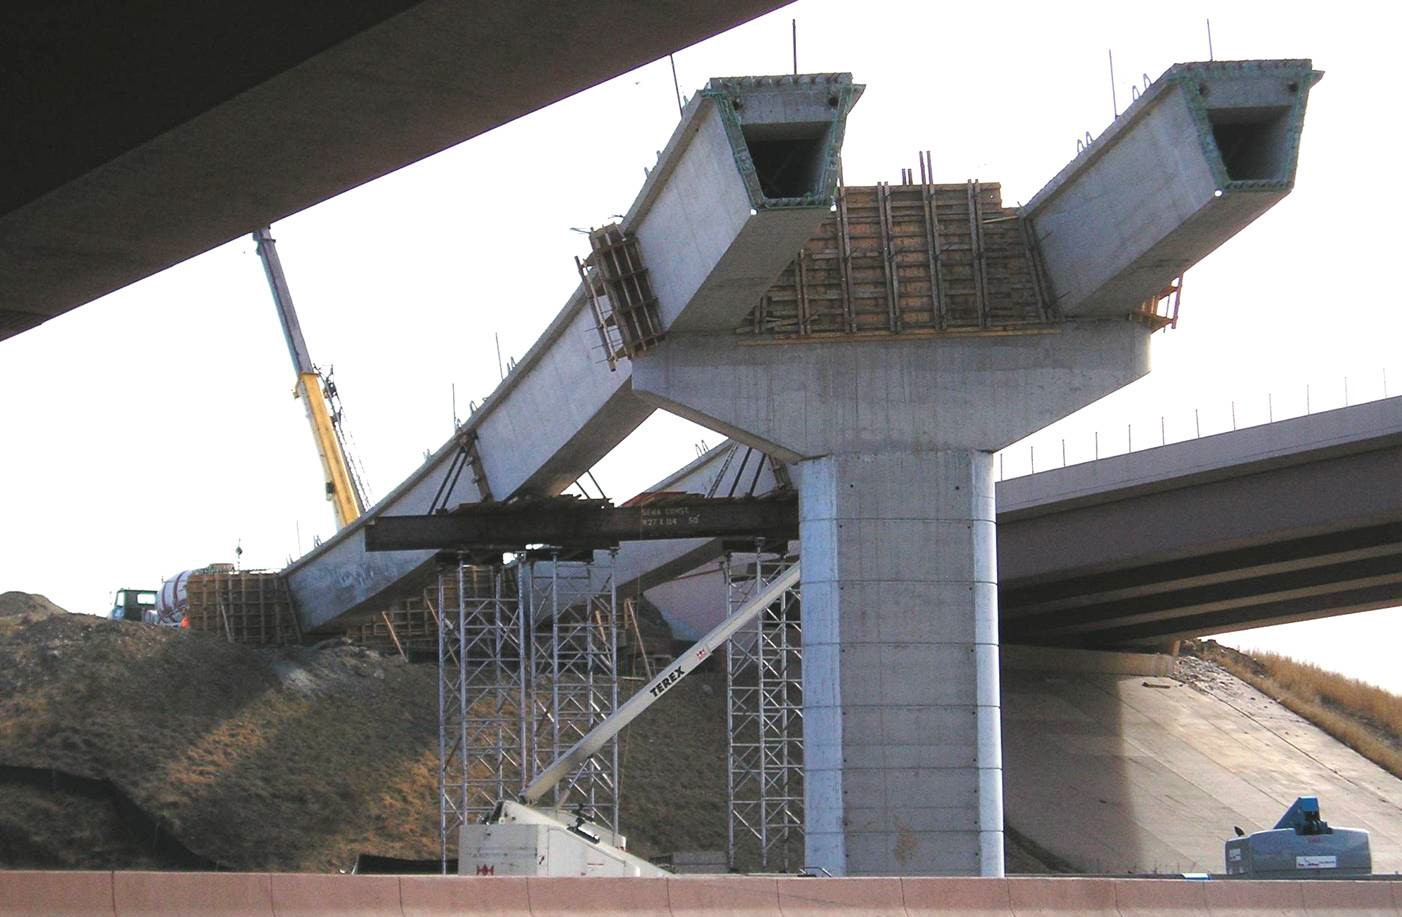
\includegraphics[width=0.65\linewidth]{spliced-concrete-curved-box.jpg}
  \caption{Spliced concrete curved boxes. (Courtesy Summit Engineering Group)}
  \label{fig:spliced-concrete-curved-box}
\end{figure}

Precast spliced girders have some similarity with segmental box girders in that both structure types consist of
smaller girder segments that are assembled and connected by posttensioning to form a final, longer girder, and both
types are erected by staged construction. However, spliced girders and segmental box girders are quite different in
the length of segments, type of splices, types of sections, tendon locations, and construction methods. Also, a
composite concrete deck is typically cast on spliced girders, while the deck slab is typically cast as an integral part of
a segmental box girder. Spliced girders use bulb-tee, I-beam, U-beam, or box shapes, while segmental box girders are
typically box shapes.



\paragraph{Cast-in-Place (CIP) Posttensioned Concrete Box Girders (on Falsework)}

Posttensioned concrete box girders cast continuously on falsework, have become very popular in several states,
particularly California, Arizona, and Nevada, and have been used in spans up to about 350 feet. This type of
construction lends itself to local construction industry practices in which contractors can economically provide the
required falsework. Similar to segmental construction, CIP on falsework offers the advantage of longer spans than
conventional girders, and can easily accommodate curved alignments. CIP construction also allows clean lines and
architectural finishes that improve the aesthetics. The use of posttensioning further enhances concrete durability by
providing a superstructure that will remain essentially crack-free under service loads. Designing the structures as a
frame and utilizing monolithic connections between the superstructure and piers also eliminates bearings, which
further eliminates associated future maintenance. A potential disadvantage of this type of construction is difficulty in
replacing the deck or widening the bridge. \cref{fig:cast-in-place-box-girder} shows a CIP box girder bridge under construction.

\begin{figure}
  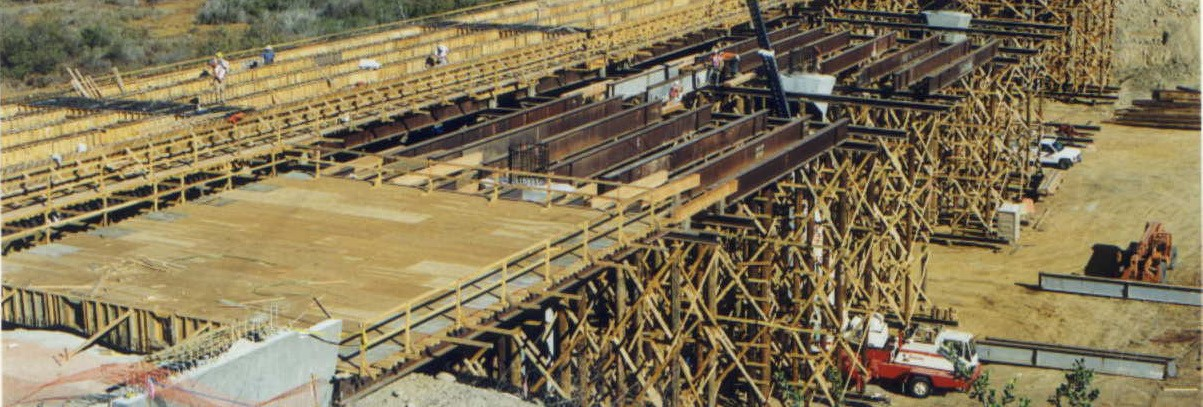
\includegraphics[width=\linewidth]{cast-in-place-box-girder.jpg}
  % \caption{Cast-in-place box girder bridge on falsework. (Courtesy Atkins North America, Inc.)}
  \caption{支架现浇箱梁}
  \label{fig:cast-in-place-box-girder}
\end{figure}

\paragraph{Segmental posttensioned concrete box girders (CIP and Precast)}

Segmental concrete box girder systems have been used when span requirements are greater than what can be
achieved with conventional stringer-type girders or spliced girders, in instances of sharp horizontal curvature, or
when special aesthetics are required. They have been economical in span ranges from about 250 feet to 500 feet.
This system is further divided into cantilever construction and span-by-span construction, and can be either precast or
cast-in-place. They can be cast to match the shape of any alignment making them particularly suited to curvature.
\cref{fig:cast-in-place-segmental} shows a cast-in-place segmental bridge recently built in Florida using balanced cantilever construction.

Segmental box girder bridges have been observed to improve deck performance due to the pre-compression of
the deck. Refer to \cref{chp:materials} on materials for additional information on these bridge deck systems and durability
issues relating to details currently in use.

\begin{figure}
  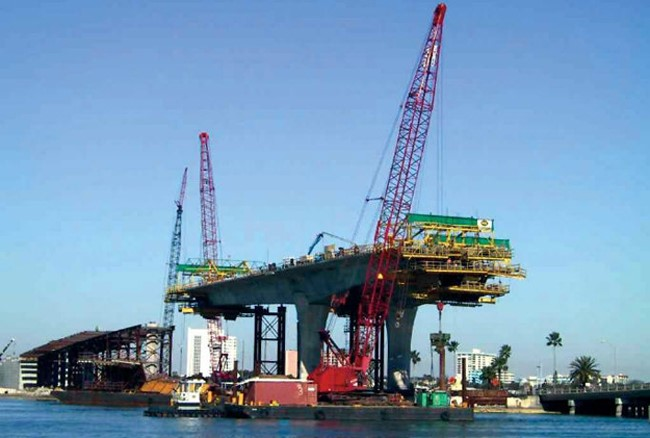
\includegraphics[height=5cm]{cast-in-place-segmental1.jpg}\hfill
  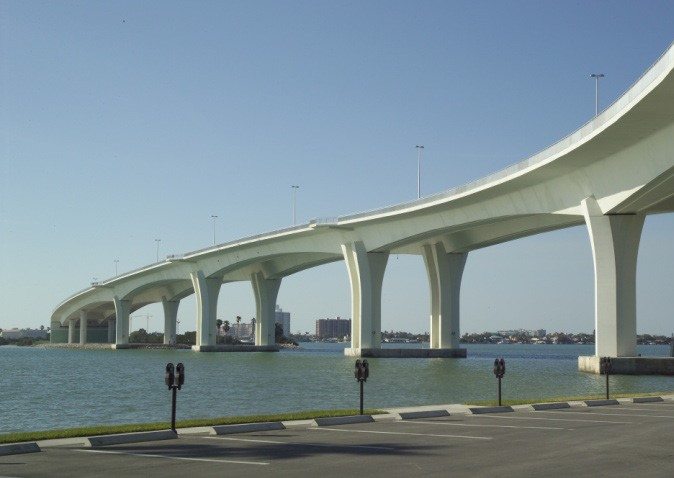
\includegraphics[height=5cm]{cast-in-place-segmental2.jpg}
  % \caption{Cast-in-place segmental concrete box system. (Courtesy HDR, right photo by John Rupe)}
  \caption{节段现浇混凝土箱梁}
  \label{fig:cast-in-place-segmental}
\end{figure}

\paragraph{Concrete Arches}

Concrete arches have been used for bridges with short spans of about 100 ft to long spans of over 1,000-ft span,
but are typically considered today only in certain long span applications because of the relative economy of I-girder
and segmental box girders in shorter spans, or when special aesthetics are required. True arches are efficient
structural systems because vertical dead load produces axial member compressive forces that are resisted by a thrust
at the arch abutments. Concrete has been useful for arches because of its inherent efficiency in compression.


Concrete arches have typically been used in deck-type systems where the arch ribs are below the deck, but they
have also been used in some through-type applications where the arch ribs extend above the deck. Deck arch
systems are either closed spandrel types or open spandrel types. Closed spandrel types typically use barrel arches
with longitudinal walls along the outside edges of the arches that are either filled or unfilled. Open spandrel types
have a series of spandrel columns that transmit deck loads to the arches.


Concrete arches in the U.S. have typically been constructed using either cast-in-place on falsework methods or cable-stayed segmental methods. \cref{fig:hoover-dam} shows the cable-stayed, cast-in-place segmental construction method used for the Hoover Dam Bypass concrete arch bridge.

\begin{figure}
  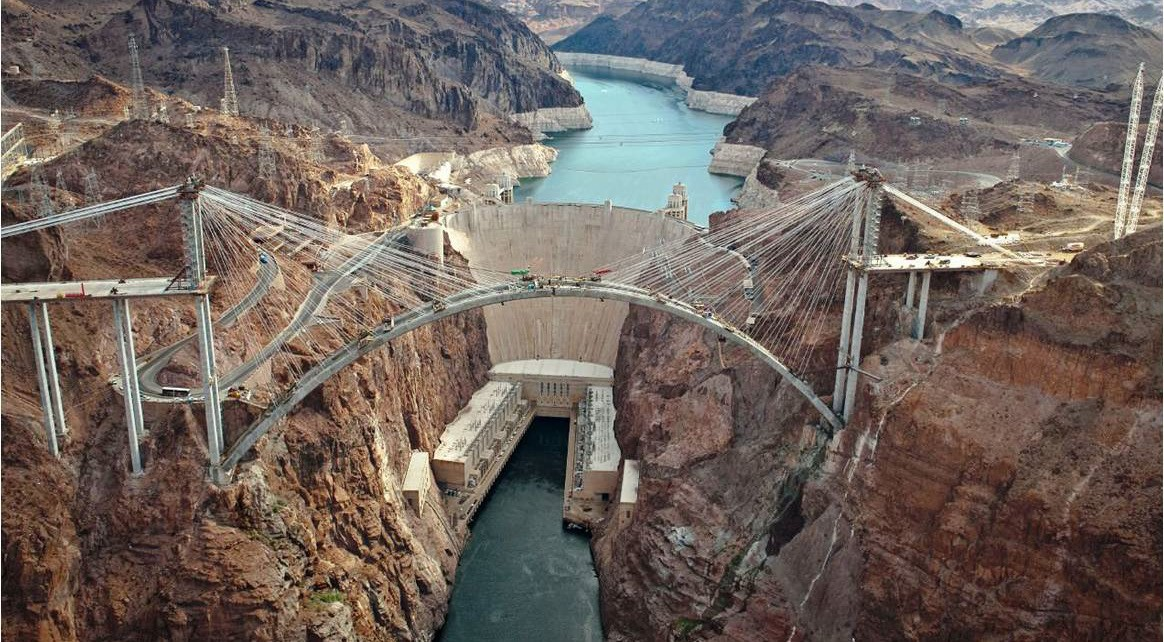
\includegraphics[width=\linewidth]{hoover-dam.jpg}
  % \caption{Hoover Dam Bypass concrete arch bridge constructed using cable-stayed segmental methods. (Courtesy HDR, photo by Keith Philpott)}
  \caption{胡佛水坝旁路采用斜拉分段法建造的混凝土拱桥}
  \label{fig:hoover-dam}
\end{figure}

\paragraph{Modular Pre-topped Concrete Girders}

These types of systems utilize precast beam elements that are fabricated with a portion of the deck in place as a unit and are erected side by side and connected with a CIP closure joint, posttensioning, composite concrete topping, or a combination of these methodologies. The precast elements commonly consist of conventionally-reinforced or prestressed sections that include T beams, double Ts, and deck bulb-tees. This system is expected to gain popularity with accelerated bridge construction as pressure mounts to expedite construction and to minimize field forming and placing of concrete. Refer to \cref{chp:bridge-decks}, \nameref{chp:bridge-decks}, for information concerning CIP closure connections.

A recent concept is the NEXT Beam (Northeast EXtreme Tee), which was developed by the Precast/Prestressed Concrete Institute North East (PCINE) along with the Departments of Transportation for New York, Connecticut, Massachusetts, Vermont, Maine, New Hampshire, and Rhode Island (Culmo and Seraderian 2010). It is a precast, prestressed double-tee section with 8-ft or 12-ft deck widths, and beam depths from 24 in. to 36 in. that is applicable for approximately 40-ft to 90-ft spans. It is available with a thick top flange that comprises the deck, or with a top flange that creates a form for a composite CIP deck. The NEXT beam is considered as an alternative to traditional adjacent concrete box beams, providing improved durability, lower cost, easier inspection and accelerated bridge construction.

% \subsection{Substructure Componet}
\subsection{下部结构\glsentrytext{component}}

The substructure component includes all structural elements required to support the superstructure and is typically defined from the underside of bridge bearings down through the foundation. The function of these elements is to transfer all vertical loads from the superstructure to the foundation supporting strata and to resist horizontal forces acting on the bridge. The transfer of load to the supporting ground can be either through spread foundations, piles, or drilled shafts, depending on the strength and stability of subsurface geotechnical conditions. This component typically includes pier and abutment subsystems, each including several elements, as shown in \cref{fig:substructure-component}.

\begin{figure}
  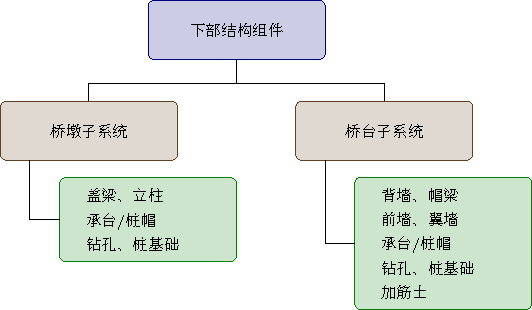
\includegraphics{component-substructure.pdf}
  % \caption{Substructure component}
  \caption{下部结构\gls*{component}}
  \label{fig:substructure-component}
\end{figure}

% \subsubsection{Piers and Bents}
\subsubsection{桥墩与排架}

Piers are intermediate supports for multi-span bridges. They can have multiple configurations, but typically fall into two major categories, piers and bents, as illustrated in \cref{fig:piertypes-multi,fig:piertypes-integral}. A pier subsystem consists of several elements, including a cap beam supporting the main load-carrying elements of the superstructure, which in turn is supported on one or more columns. The columns are supported by foundations that are typically located at or below the finish grade of the adjacent ground. The foundation can be a footing bearing directly on rock or soil, or a deep foundation using piles or drilled shafts.

T-piers are examples of single column piers with a cap element. Solid- or wall-type piers are also single column piers, but are wide enough to support the superstructure without having a separate cap element.

A bent consists of a cap beam supporting the main load-carrying elements of the superstructure, which in turn is supported directly on deep foundation elements such as piles or drilled shafts that extend up from finish grade. In some cases, the term “bent” is also used to describe a multi-column pier.

Common practice is to construct piers with reinforced concrete, although some steel piers with pier caps have been used. When deep foundations are required to support the bent caps, they normally consist of timber, prestressed concrete square, solid round or hollow cylinder piles, CIP concrete drilled shafts, or steel HP or steel pipe sections.

Modular, precast concrete pier elements have also been used for accelerated construction.

\begin{figure}
  \begin{minipage}{0.48\linewidth}\centering
    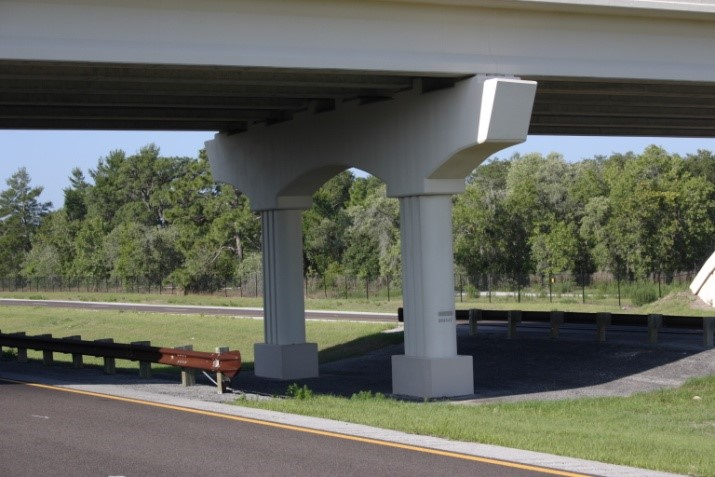
\includegraphics[height=4.5cm]{piertype1.jpg}
    \subcaption{多柱式桥墩}
  \end{minipage}\hfil
  \begin{minipage}{0.48\linewidth}\centering
    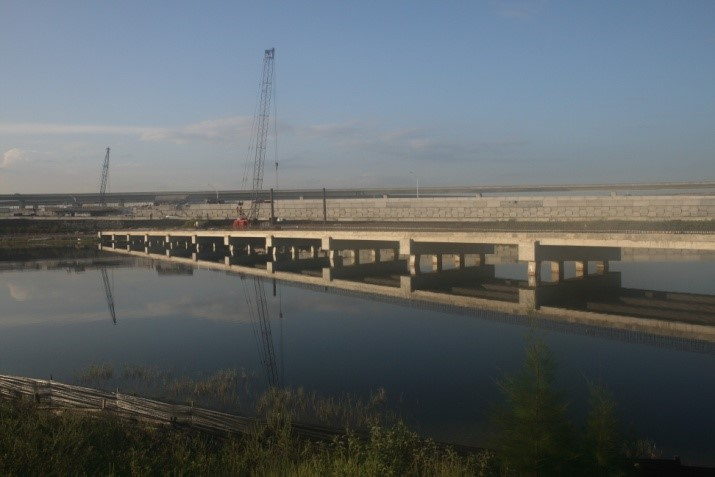
\includegraphics[height=4.5cm]{piertype2.jpg}
    \subcaption{排架桩}
  \end{minipage}
  % \caption{Pier types: multi-column supported pier and pile bent. (Courtesy Atkins North America, Inc.)}
  \caption{桥墩类型:多柱式桥墩和排架桩。}
  \label{fig:piertypes-multi}
\end{figure}

Integral pier cap construction was also developed as a way to avoid sharp skews or associated longer spans in interchange ramp bridges, and to lower overpass profiles. Integral pier caps also have the advantage of eliminating bearings, which can minimize future maintenance requirements. \cref{fig:piertypes-integral} shows a ramp bridge with conventional stacked T-pier construction and a similar ramp bridge with integral pier construction. Integral pier system is advantageous in seismic areas by integrating the super structure and substructure and creating frame action.

\begin{figure}
  \begin{minipage}{0.48\linewidth}\centering
    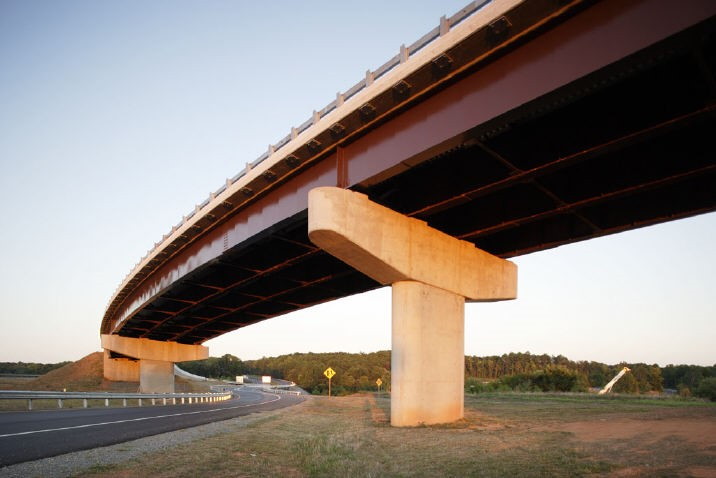
\includegraphics[height=4.5cm]{piertype3.jpg}
    \subcaption{常规 T 型桥墩的匝道桥}
  \end{minipage}\hfil
  \begin{minipage}{0.48\linewidth}\centering
    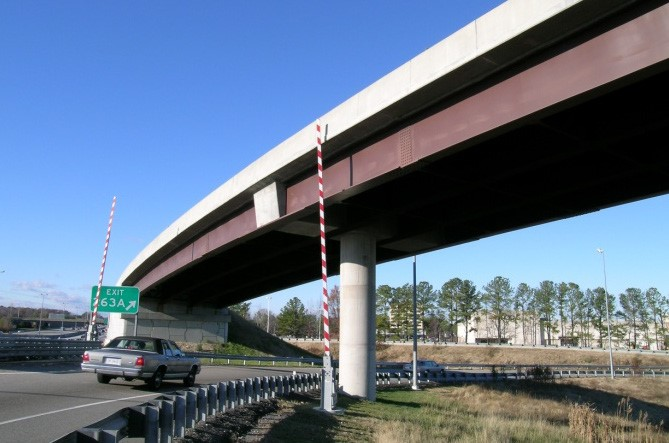
\includegraphics[height=4.5cm]{piertype4.jpg}
    \subcaption{整体式桥墩的匝道桥}
  \end{minipage}
  % \caption{Conventional and integral pier types. (Courtesy HDR)}
  \caption{常规和整体式桥墩类型}
  \label{fig:piertypes-integral}
\end{figure}

% \subsubsection{Abutments}
\subsubsection{桥台}
Abutments are provided in multiple configurations, but can be defined in two major categories as illustrated in \cref{fig:abutmenttypes}:
\begin{itemize}
  \item Stub or spill-through abutments, and
  \item Full abutments.
\end{itemize}

\begin{figure}
  \begin{minipage}{0.48\linewidth}\centering
    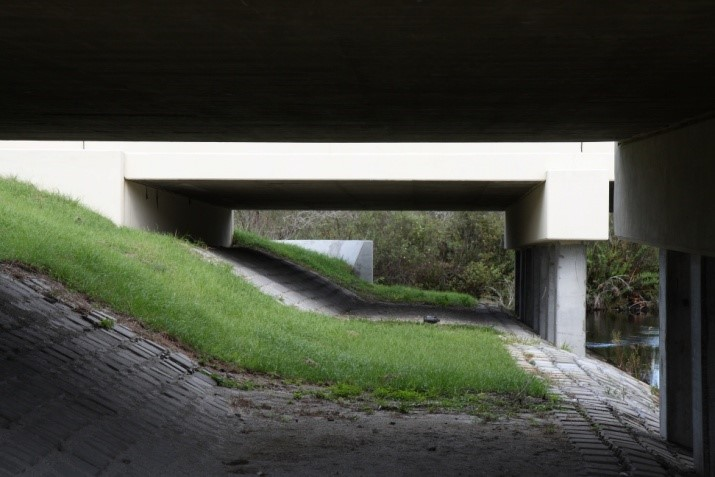
\includegraphics[height=4.5cm]{abutment1.jpg}
    % \subcaption{Stub or spill-through abutment.}
    \subcaption{墩式溢流型桥台}
  \end{minipage}\hfil
  \begin{minipage}{0.48\linewidth}\centering
    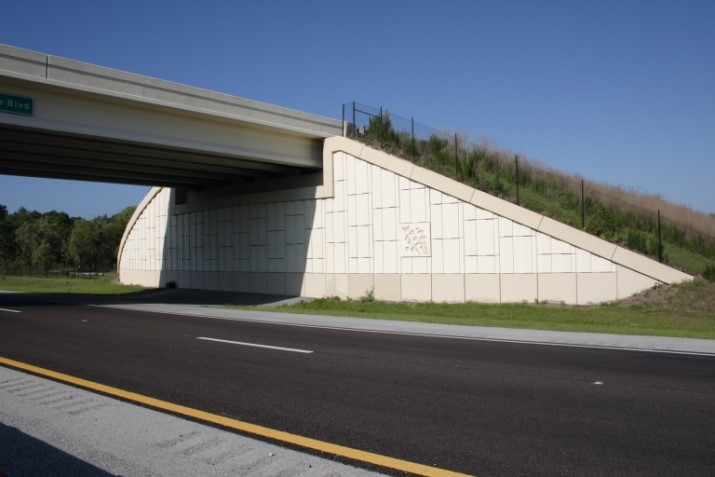
\includegraphics[height=4.5cm]{abutment2.jpg}
    % \subcaption{MSE full abutment.}
    \subcaption{全 \acrshort*{mse} 桥台.}
  \end{minipage}
  % \caption{Abutment types. (Courtesy Atkins North America, Inc.)}
  \caption{桥台类型}
  \label{fig:abutmenttypes}
\end{figure}

Stub abutments are characterized by sloped embankments under the end span of the bridge and provide support to the superstructure through a shallow bent cap resting on a pile foundation.

Traditionally, full abutments are characterized by a vertical wall that retains the embankment fill and also transfers the bridge load to the supporting foundation at the base of the wall. Full abutments can also be in the form of a \acrfull{mse} system, which employs a fascia wall connected to a system of reinforcing elements in multiple layers that work with the backfill material to create a composite soil mass. This composite soil mass can then support vertical load and/or act as an earth retention system. There are two types of MSE abutments: true or mixed (Anderson and Brabant 2010). In a true MSE abutment, the bridge superstructure is supported on spread footings bearing directly on the top of the reinforced soil mass. In a mixed MSE abutment, a shallow bent cap with a row of piles is used to support the superstructure behind the MSE fascia wall, and the reinforced soil mass is used to retain the fill behind and adjacent to the end of the bridge. A MSE full abutment is pictured in \cref{fig:abutmenttypes}.

Another recent form of abutment system is the \acrfull{grsibs}, which is described in FHWA publication FHWA-HRT-11-027 (Adams et al. 2011). This is a relatively new abutment system that has been used for accelerated bridge construction, and typically for short spans up to about 140 feet. The abutment uses alternating thin layers of compacted fill and geosynthetic reinforcement sheets that combine to form a reinforced soil mass foundation that directly supports the bridge superstructure without the need for piles. The geosynthetic reinforcement is connected into layers of precast facing blocks that are placed with the reinforcement and soil backfill. Once completed, the reinforced soil mass is ready to support the bridge.

Traditional abutments are typically concrete construction. When deep foundations are required to support the bent caps, they normally consist of timber, prestressed concrete square, solid round or hollow cylinder piles, CIP concrete drilled shafts, or steel HP or pipe pile sections.

Types of abutments used also characterize the way the entire bridge system responds to thermally-induced longitudinal movements. There are three distinct abutment types:
\begin{itemize}
  \item Integral abutment,
  \item Semi-integral abutment, and
  \item Abutment using expansion devices.
\end{itemize}

In integral abutment systems, are attached directly to abutment, and thermally-induced longitudinal movements are accommodated by flexibility of the piles. The piles are subject to both axial and flexural moments. In semiintegral abutment systems, girders and piles are not directly connected and the bearings used to support girders and piles are mainly subject to axial loads. Integral and semi-integral abutment systems are part of different continuous bridge systems. \cref{chp:jointless-bridge} provides a more in-depth discussion, as well as detailed design provisions for integral and semi-integral abutment systems.


\section{Factors Affecting Service Life}
\label{sec:factors-affect-sl}

All of the elements, components, and subsystems that make up the overall bridge system are adversely affected in various degrees by both external and internal factors that contribute to reduced service life. External factors typically refer to loads or hazards, which can be both natural and man-made. Internal factors can pertain to such items as structure type (e.g. fracture critical), materials, and design/details.

Following is a discussion of critical factors that affect bridge service life using a fault tree analysis approach. Section 2.3.1 discusses factors that affect the overall bridge system. The following sections, 2.3.2 through 2.3.4, address specific factors affecting deck, superstructure, and substructure components. Section 2.4 addresses options to avoid or mitigate these factors.

\begin{figure}
  % \includegraphics[width=\linewidth]{factor-service-life.pdf}
  \caption{Factors affecting service life.}
  \label{fig:factor-service-life}
\end{figure}

\subsection{Bridge System Fault Tree Analysis}

\cref{fig:factor-service-life} shows the initial fault tree diagram that identifies factors affecting service life for a complete bridge system. (A detailed discussion of the fault tree process is included in \cref{chp:general-frame}.) The diagram identifies causes of, or factors affecting service life and categorizes them for consideration. In following sections, these categories are successively sub-categorized at descending levels to identify multiple contributing factors. The fault tree analysis is then continued until the basic events or lowest levels of resolution are reached and discussed. The lowest level or basic events require strategies for mitigations.

\subsubsection{Obsolescence or Deficiency}

At the highest fault level, reduced service life of a bridge system can be attributed to either obsolescence or deficiency. Obsolescence refers to reduced service life of a bridge due to issues related to how it functions, which can be further categorized as:
\begin{itemize}
  \item Operational issues related to reduced traffic capacity and safety,
  \item Physical issues related to span layout and clearances, or
  \item Loading issues related to increases in design live load.
\end{itemize}

Many bridges are replaced because of functional issues well before their full-potential service life is achieved. Significant increases in corridor traffic demand, caused by such factors as urban planning, land use, and development, can ultimately result in the functional inability of a bridge to provide required level of service, necessitating bridge widening or replacement. Vertical clearance limitations sometimes prevent existing bridges from being widened. Increased corridor traffic can also require replacement of overpass bridges to accommodate widened roadways and increased span requirements below. Major interchanges are sometimes reconstructed because of the need for increased traffic capacity.

Often, safety issues relating to inadequate lane and shoulder widths, sharp curves, and inadequate sight distances have a significant effect on service life. Changes in design live load over the life of a bridge can affect service life as it relates to the structure’s ability to safely accommodate increased load.

Service life design considerations should evaluate the potential of future operational needs, and how those needs might impact the service life of the planned facility. Risks of future obsolescence should be considered and appropriate choices should be made concerning mitigation or acceptance. Those choices should be incorporated into the design as appropriate considering life-cycle cost analysis.

Deficiency refers to reduced service life of a bridge due to damage or deterioration that can be caused by a number of primary factors and sub-factors, each of which can lead to reduced service life if un-mitigated. Deficiency can occur in all three bridge components: deck, superstructure, and substructure. In \cref{fig:factor-service-life}, the fault tree continues below the superstructure component, but it applies equally to all three components.

Within a bridge system, the interaction between components, deficiencies, or failures within a particular component can have a significant effect on other components. A primary example is deterioration of superstructure and substructure below leaking joints in the deck component (see Section 2.3.1.3.1). Another example is damage to substructure and other superstructure elements caused by failed bearings in the superstructure component (see Section 0)

Deficiency can be further attributed to any of three major causes:
\begin{itemize}
  \item Load-induced,
  \item Natural or man-made hazards, or
  \item Defects in production/operation.
\end{itemize}

\subsubsection{Reduced Service Life due to Loads}

Load-induced deficiencies can be further categorized as those caused by traffic-induced loads or systemdependent loads (see \cref{fig:load-induced-deficiencies}). The fault tree is continued for each of these load types to identify the basic or lowest levels causing damage or deterioration.

\begin{figure}
  % \includegraphics[width=\linewidth]{load-induced-deficiencies.pdf}
  \caption{Load-induced deficiencies}
  \label{fig:load-induced-deficiencies}
\end{figure}

\paragraph{Traffic-Induced Loads}

Traffic-induced loads include the effects of truck and other vehicle traffic that are applied to the bridge deck and transmitted throughout the bridge system. Traffic load can ultimately cause damage to bridge elements through
fatigue, overload, or wear.

\begin{description}
  \item [Fatigue] is structural damage to an element resulting from cyclic loading that results in the initiation and  propagation of cracks, and can occur at stress levels considerably below the yield stress. Although fatigue can occur in reinforced concrete and structural steel elements, it is more predominant in steel elements. \cref{chp:materials} on materials discusses fatigue deterioration in reinforced concrete.

  Early-welded steel structures have a history of cracking at certain types of weld details due to load-induced and distortion-induced fatigue. Newer design provisions and recommended details have been developed that provide solutions for both load-induced and distortion-induced fatigue that will achieve desired service life. Section 2.3.3.1.1 provides additional information of fatigue in steel structures, and \cref{chp:fatigue-fracture-steel-structures} provides a comprehensive discussion on fatigue and fracture in steel bridges.
  \item [Overload] refers to element overstress or damage resulting from over-weight vehicles that exceed maximum gross vehicle weight restrictions or individual axle or tire restrictions. Overload often results from illegal, nonpermitted vehicles and is the third leading cause of bridge failure in the U.S. behind hydraulic and impact causes (Wardhana and Hadipriono, 2003). Overload produces higher stress in members than what was considered in design,
  and can significantly reduce safety factors against failure, and can cause cracking in concrete elements. Multiple applications can also affect fatigue behavior and also result in excessive deflection that can affect certain elements, particularly in cases of differential deflection.

  Because overload occurs on many bridges, the risk of overload should be considered on certain vehicular routes when planning new bridges. It may also be necessary to consider special owner-specified loads to avoid or mitigate this risk.
  \item [Wear] refers to element damage and gradual loss of material caused by friction or rubbing. Decks are susceptible to wear from vehicle tires, especially with the use of studs or chains. Deck wear and abrasion is further discussed in \cref{chp:bridge-decks}. Wear has been a factor in steel structures, particularly on pins and pin plates in connections, and in bearings, with surface wear in sliding bearings, brass sealing ring wear in pot bearings, and pin wear in steel bearings.
\end{description}

\paragraph{System-Induced Loads}
System-induced loads include the effects of the bridge system configuration on the behavior of the structure. These effects are accentuated by restraints provided through bridge boundary conditions and can result in significant locked-in stresses. The system-induced loads can be the result of movements due to time-dependent material properties, thermal movements, or system framing restraint.

\begin{description}
  \item [Time-dependent material properties] refers mainly to shrinkage and creep-related deformations in restrained
  concrete elements and can result in concrete cracking. This phenomenon is discussed further in \cref{chp:bridge-decks} for bridge
  decks and in \cref{chp:materials} for concrete materials in general.
  \item [Thermal Conditions] refers to effects caused by temperature change, which can result in significant stresses in
  restrained structural members, and can be as large as live load stresses in some cases. The effects can be the result of
  uniform stress across a bridge member, or the result of a temperature gradient throughout the depth of a member.
  \item [System-framing restraint] refers to effects caused by boundary condition restraints that prevent normal or
  intended structural behavior. Improper function or seizing of bearings can result in unintended movement restraint,
  which can further cause pier cracking and distress. Another example occurs at ends of skewed integral abutments,
  where lateral movement resulting from the skew can cause cracking and distress in corner details if adequate
  clearance is not provided to allow for the movement.
\end{description}

\subsubsection{Reduced Service Life due to Natural or Man-Made Hazards}

Environmental hazards from both natural and man-made sources can have a significant influence on bridge service life. These also include effects from areas with adverse thermal climate, coastal climates, and chemical climates, as well as from chemical properties of the materials themselves. Other hazards such as hydraulic action, collisions, fire/blast, or seismic events can also have considerable effect. These natural and man-made hazards are introduced in the fault tree shown in \cref{fig:natural-man-made-hazards}.

\begin{figure}
  % \includegraphics[width=\linewidth]{natural-man-made-hazards.pdf}
  \caption{Natural or man-made hazards}\label{fig:natural-man-made-hazards}
\end{figure}

\paragraph{Thermal Climate}
Deicing salts corrosion. Bridge service life is typically severely affected in cold, wet climates due to heavy use of roadway deicing salt. Salt-contaminated moisture penetration directly affects bridge deck service life by initiating and propagating corrosion in unprotected reinforcing steel, and by accelerating concrete deterioration due to cracking and freeze/thaw damage. All unprotected bridge elements below open or leaking deck joints are subject to saltcontaminated roadway drainage, which causes unprotected structural steel corrosion, concrete reinforcing bar corrosion, and associated concrete cracking and spalling.

On overpass bridges, salt spray rising from roadways below affects superstructures and undersides of decks,
causing concrete penetration and corrosion of unprotected reinforcing, and corrosion of unprotected structural steel.
The salt spray from vehicles passing underneath the bridge can also affect the service life of weathering steel by
keeping the steel continuously wet.

Decks, barriers and deck joints are also susceptible to damage from snow plows used to clear roadways for
traffic.

Freeze/Thaw. Water absorbed into concrete surfaces and contained in cracks can freeze in cold weather
conditions. The frozen water tends to expand causing stresses within the concrete. Cyclic freezing and thawing of the
water absorbed in the deck surface fatigues the concrete, resulting in cracking, scaling, and spalling. Refer to
\cref{chp:materials} on materials for additional information on freeze/thaw in concrete.

\paragraph{Coastal Climate}
Salt water/spray corrosion. Coastal saltwater environments also have severe effects on bridge service life due
to wetting and chloride penetration causing corrosion of unprotected reinforcing, and corrosion of unprotected
structural steel.

Structures in these areas are subjected to a chloride-laden saltwater environment and a combination of wind and
wave action that causes these chlorides to become airborne as salt spray. The susceptibility of various bridge
components to these environmental influences depends on their degree of direct contact or their height above the
water elevation. Pier columns with direct contact in areas of continual wetting are most susceptible to damage.

Wave action hitting substructure units and seawalls or abutments under the bridge also tend to cause the salt
spray to explode upward, wetting the bottoms of lower level superstructures and decks. The salt spray can also
deposit itself on the bridge deck surface, particularly on windy days. The salt spray wets the surfaces leaving a
chloride residual that can absorb into the concrete, resulting in reinforcement corrosion that in turn causes cracking, spalling, and/or delamination. The wet salt spray can also be deposited on the sides of structural steel members
affecting service life of coatings, and directly causing and accelerating steel corrosion.

Humidity. High humidity in coastal regions also results in cyclic wetting and drying of bridge surfaces. Concrete
materials sensitive to repeated wetting, such as those in which reactive aggregates are utilized, can have an adverse
effect on concrete elements. Continuous wetting and drying also affects coatings on structural steel members and
causes steel corrosion.

\paragraph{Chemical Climate}

Corrosion-inducing chemicals. Chemical climate influences on bridge service life performance can be
attributed primarily to airborne corrosion-inducing chemicals as a result of nearby industrial facilities such as
chemical plants or oil and coal-burning facilities. \cref{chp:materials} provides further discussion on chemical influences on
concrete, and \cref{chp:corrosion-prevention-steel-bridge} discusses the influence of corrosion-inducing chemicals with respect to steel coatings and
steel corrosion.

Sulfate attack. Exposure to sulfates can cause expansion of concrete material that can cause spalling and
cracking, and the loss of bond strength between the cement paste and aggregate. Refer to \cref{chp:materials} for additional
information on sulfate attack in concrete.


\paragraph{Reactive Materials}

Reactive ingredients with the concrete mix can affect concrete service life performance by altering the
volumetric stability of the concrete mix design. These influences primarily occur naturally.

Alkali-silica reactivity (ASR) results in swelling of aggregate particles within concrete that can lead to spalling,
cracking and general concrete deterioration. \cref{chp:materials} provides additional information on ASR in concrete.

Alkali-carbonate reactivity (ACR) results in aggregate expansion within concrete that can lead to spalling,
cracking and general concrete deterioration. Refer to \cref{chp:materials} for additional information on ACR in concrete.

\paragraph{Hydraulic Action}

Hydraulic action is the leading cause of bridge failure in the United States (Wardhana and Hadipriono 2003).
The two principal base elements are flood/storm surge and scour.

Flood/storm surge. Floods and storm surges can significantly affect bridge service life, and can dislodge spans
from their bearings and wash them away. Storm surges during major hurricanes are most often the cause of bridge
damage, as occurred in 2005 during Hurricane Katrina, which devastated the Gulf coastline from Louisiana to the
Florida Panhandle, and damaged nearly 45 bridges (Padgett et al. 2008). Most of the damaged bridges were adjacent
to water and damage resulted from storm surge-induced loading. Much of the damage was to superstructures, where
typical damage included unseating or shifting of decks and failure of bridge parapets. Several bridges suffered
damage due to impact from loose barges and debris. The most common severe failure was unseating, which often
occurred in low elevation spans. The deck displacements were attributed primarily to a combination of buoyant
forces and pounding waves. Superstructure damage largely depended on the connection type between the decks and
bents and the bearings often provided no apparent positive connection between the superstructure and substructure.

\cref{fig:bridges-washed-out} shows the I-10 bridges across Escambia Bay in Florida that were dislodged during a storm in 2006.
Damage due to superstructure unseating was similar to that experienced in the Katrina bridge damages.

Bridges with low vertical clearance over a waterway can also be vulnerable to damage resulting from debris flow
in a flood.

\begin{figure}
  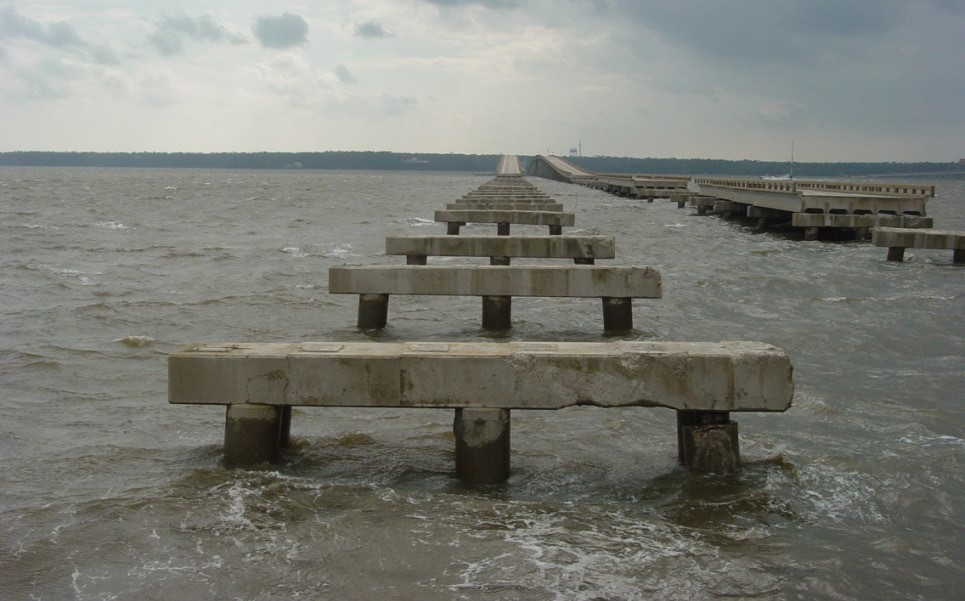
\includegraphics[width=0.5\linewidth]{bridges-washed-out.jpg}
  % \caption{Florida I-10 Escambia Bay bridges washed out during storm. (Courtesy Florida DOT)}
  \caption{佛罗里达州 I-10 埃斯坎比亚湾桥梁在暴风雨中被冲毁}
  \label{fig:bridges-washed-out}
\end{figure}

Scour. Scour is defined as the erosion or removal of streambed or bank material from bridge foundations due to flowing water. Although scour can occur at any time, bridge scour most often results during floods where swiftly flowing water has more energy than calm water to lift and carry sediment down river. A hole is created adjacent to the pier or abutment when material is washed away from the river bottom exposing or undermining footings, which can compromise the integrity of the structure and lead to failure. \cref{fig:abutment-scour} shows an example of abutment scour. See Section 2.3.4 for factors affecting service life of bridge substructures.

\begin{figure}
  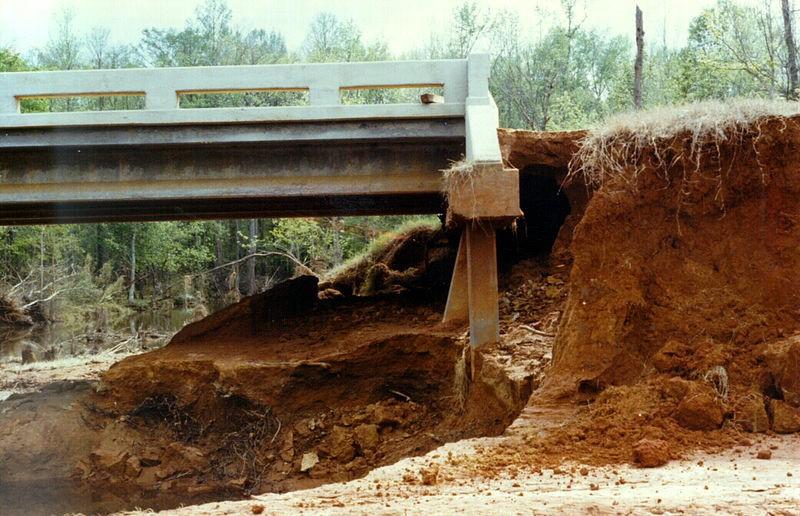
\includegraphics[width=0.5\linewidth]{abutment-scour.jpg}
  % \caption{Abutment scour. (Courtesy U.S. Geological Survey, photo by Bill Colson)}
  \caption{桥台冲刷}
  \label{fig:abutment-scour}
\end{figure}

\paragraph{Extreme Events}
\subparagraph{Vehicle/Vessel Collision}
Vehicle/vessel collision is second to hydraulic effects as the leading cause of bridge failures (Wardhana and Hadipriono 2003). Bridges crossing other roadways with minimum or low clearance are subject to various types of vehicle collision, particularly involving over-height vehicles. \cref{fig:bridge-impacted-by-truck} shows the effects of a collision in which a truck transporting a hydraulic crane with the boom inadvertently raised struck a concrete bridge and cut halfway through the entire width of the superstructure. Piers with minimum offset from edge of roadway or shoulder are also subject to vehicle collision if not adequately protected by barriers.

The risk of vehicle impact should be considered in the design of new bridges, particularly bridges crossing heavy
truck routes where a greater probability exists for over-height vehicles, and where there has been a history of impacts
from over-height vehicles. Possible mitigation strategies include:
\begin{itemize}
  \item Using higher clearances,
  \item Using sacrificial beams to protect load carrying members, and
  \item Using laser detection systems that set off warning signals if an over-height vehicle is detected.
\end{itemize}

\begin{figure}
  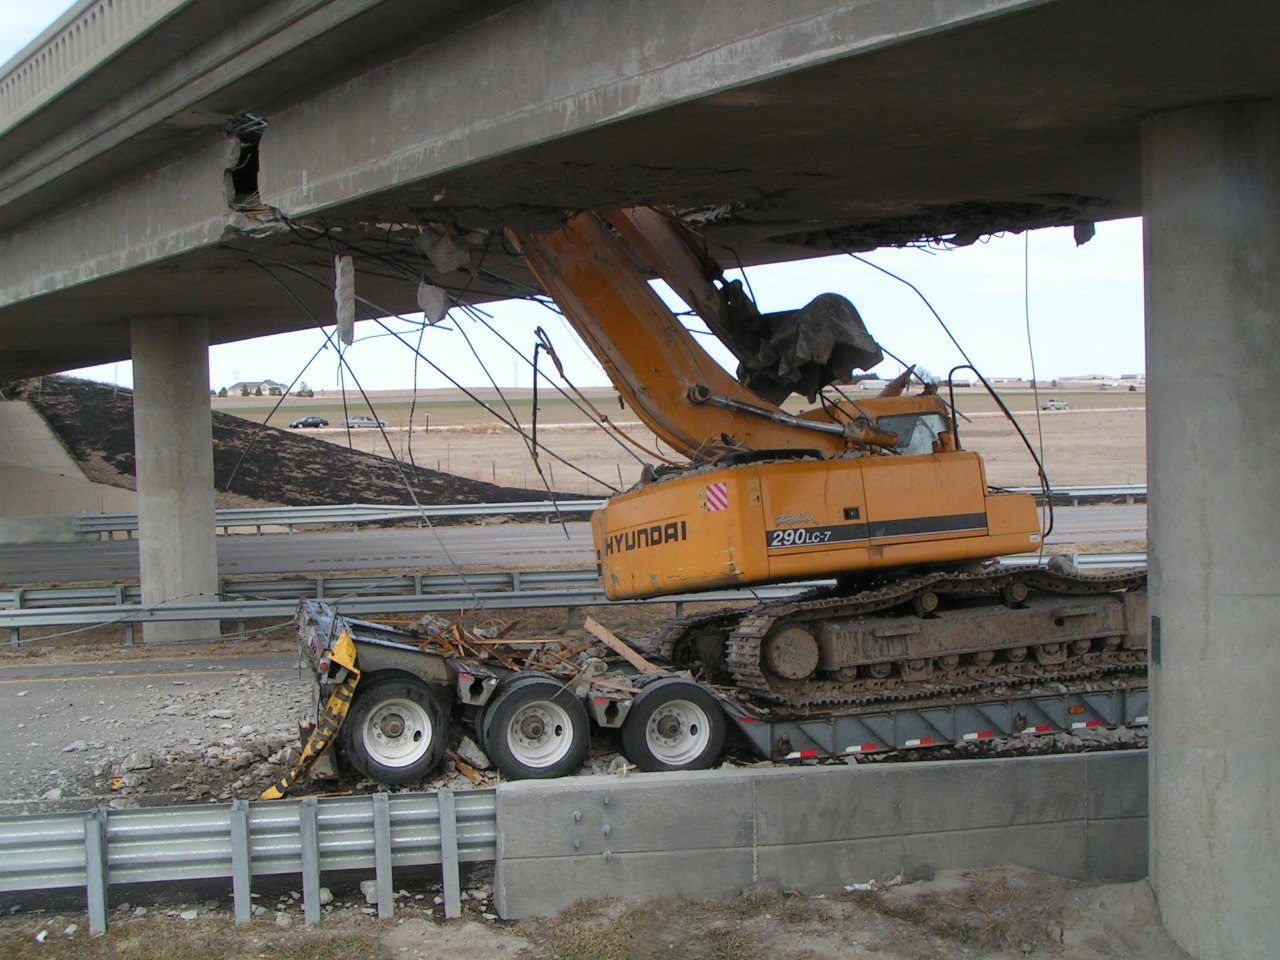
\includegraphics[height=6.5cm]{bridge-impacted-by-truck1.jpg}\hfill
  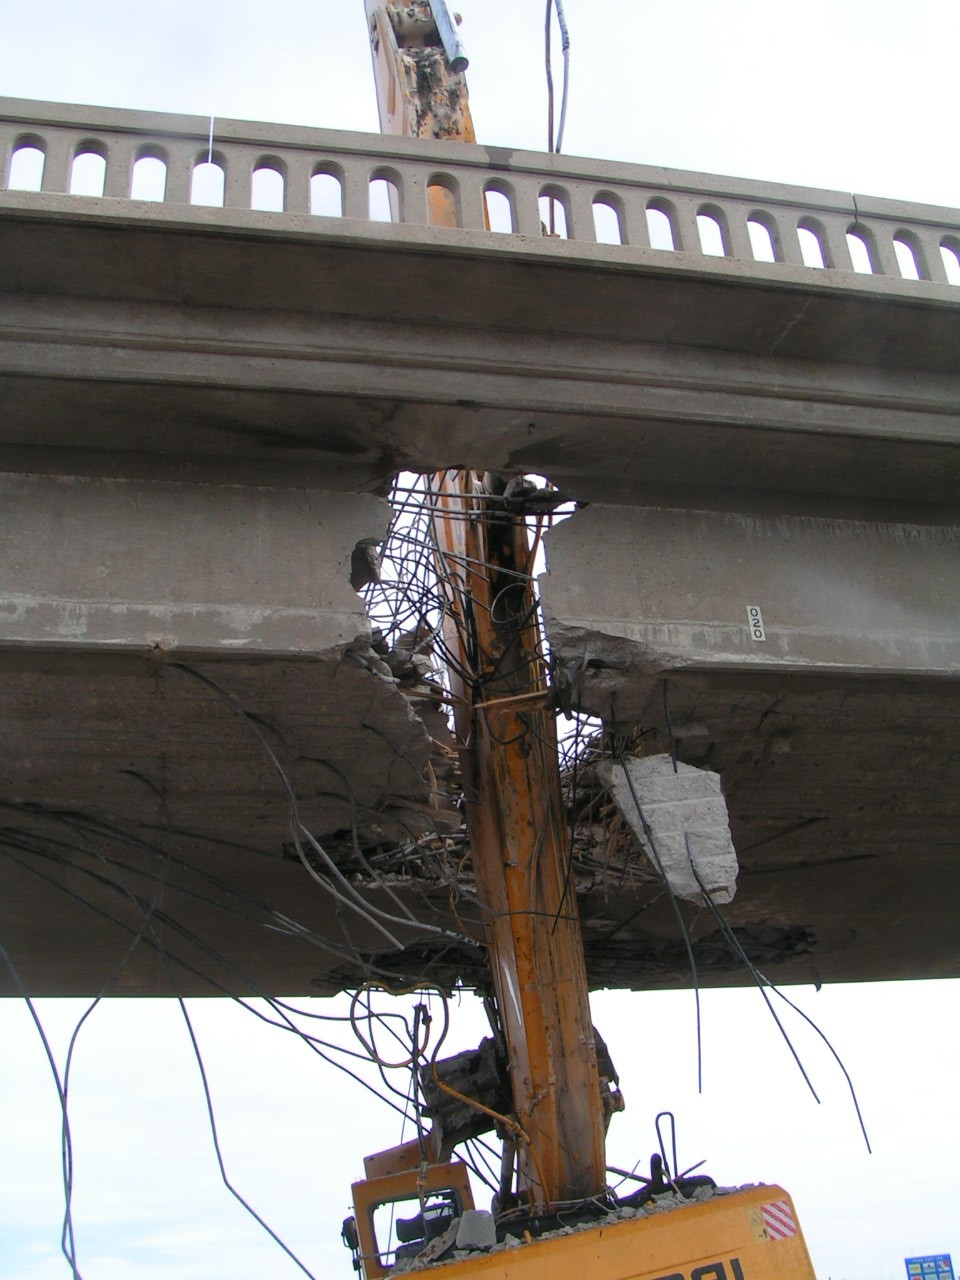
\includegraphics[height=6.5cm]{bridge-impacted-by-truck2.jpg}
  % \caption{Bridge impacted by truck transporting hydraulic crane. (Courtesy Kansas DOT)}
  \caption{运输液压起重机的卡车撞击桥梁}
  \label{fig:bridge-impacted-by-truck}
\end{figure}

Bridges crossing water bodies or waterways are subject to ships colliding with either piers or superstructure.
They are rarely occurring extreme events, but have potentially high consequences. \cref{fig:ship-collision} shows the aftermath
of a ship collision with the original Sunshine Skyway Bridge in Florida. The ship collided with one of the end piers
in the main channel 3-span unit, took out the pier and subsequently the superstructure unit.

Considerations for new bridges should evaluate span openings required for safe navigation, including horizontal
and vertical clearances, and consider appropriate mitigation measures to reduce the risk of collision. Adequate
fender systems or other pier protection devices also need to be considered where there is risk of ship collision.

The current AASHTO LRFD Bridge Design Specifications (LRFD Specifications) provide requirements for new bridge design for both vehicle and ship impact \cite{aashto2012l}.

\begin{figure}
  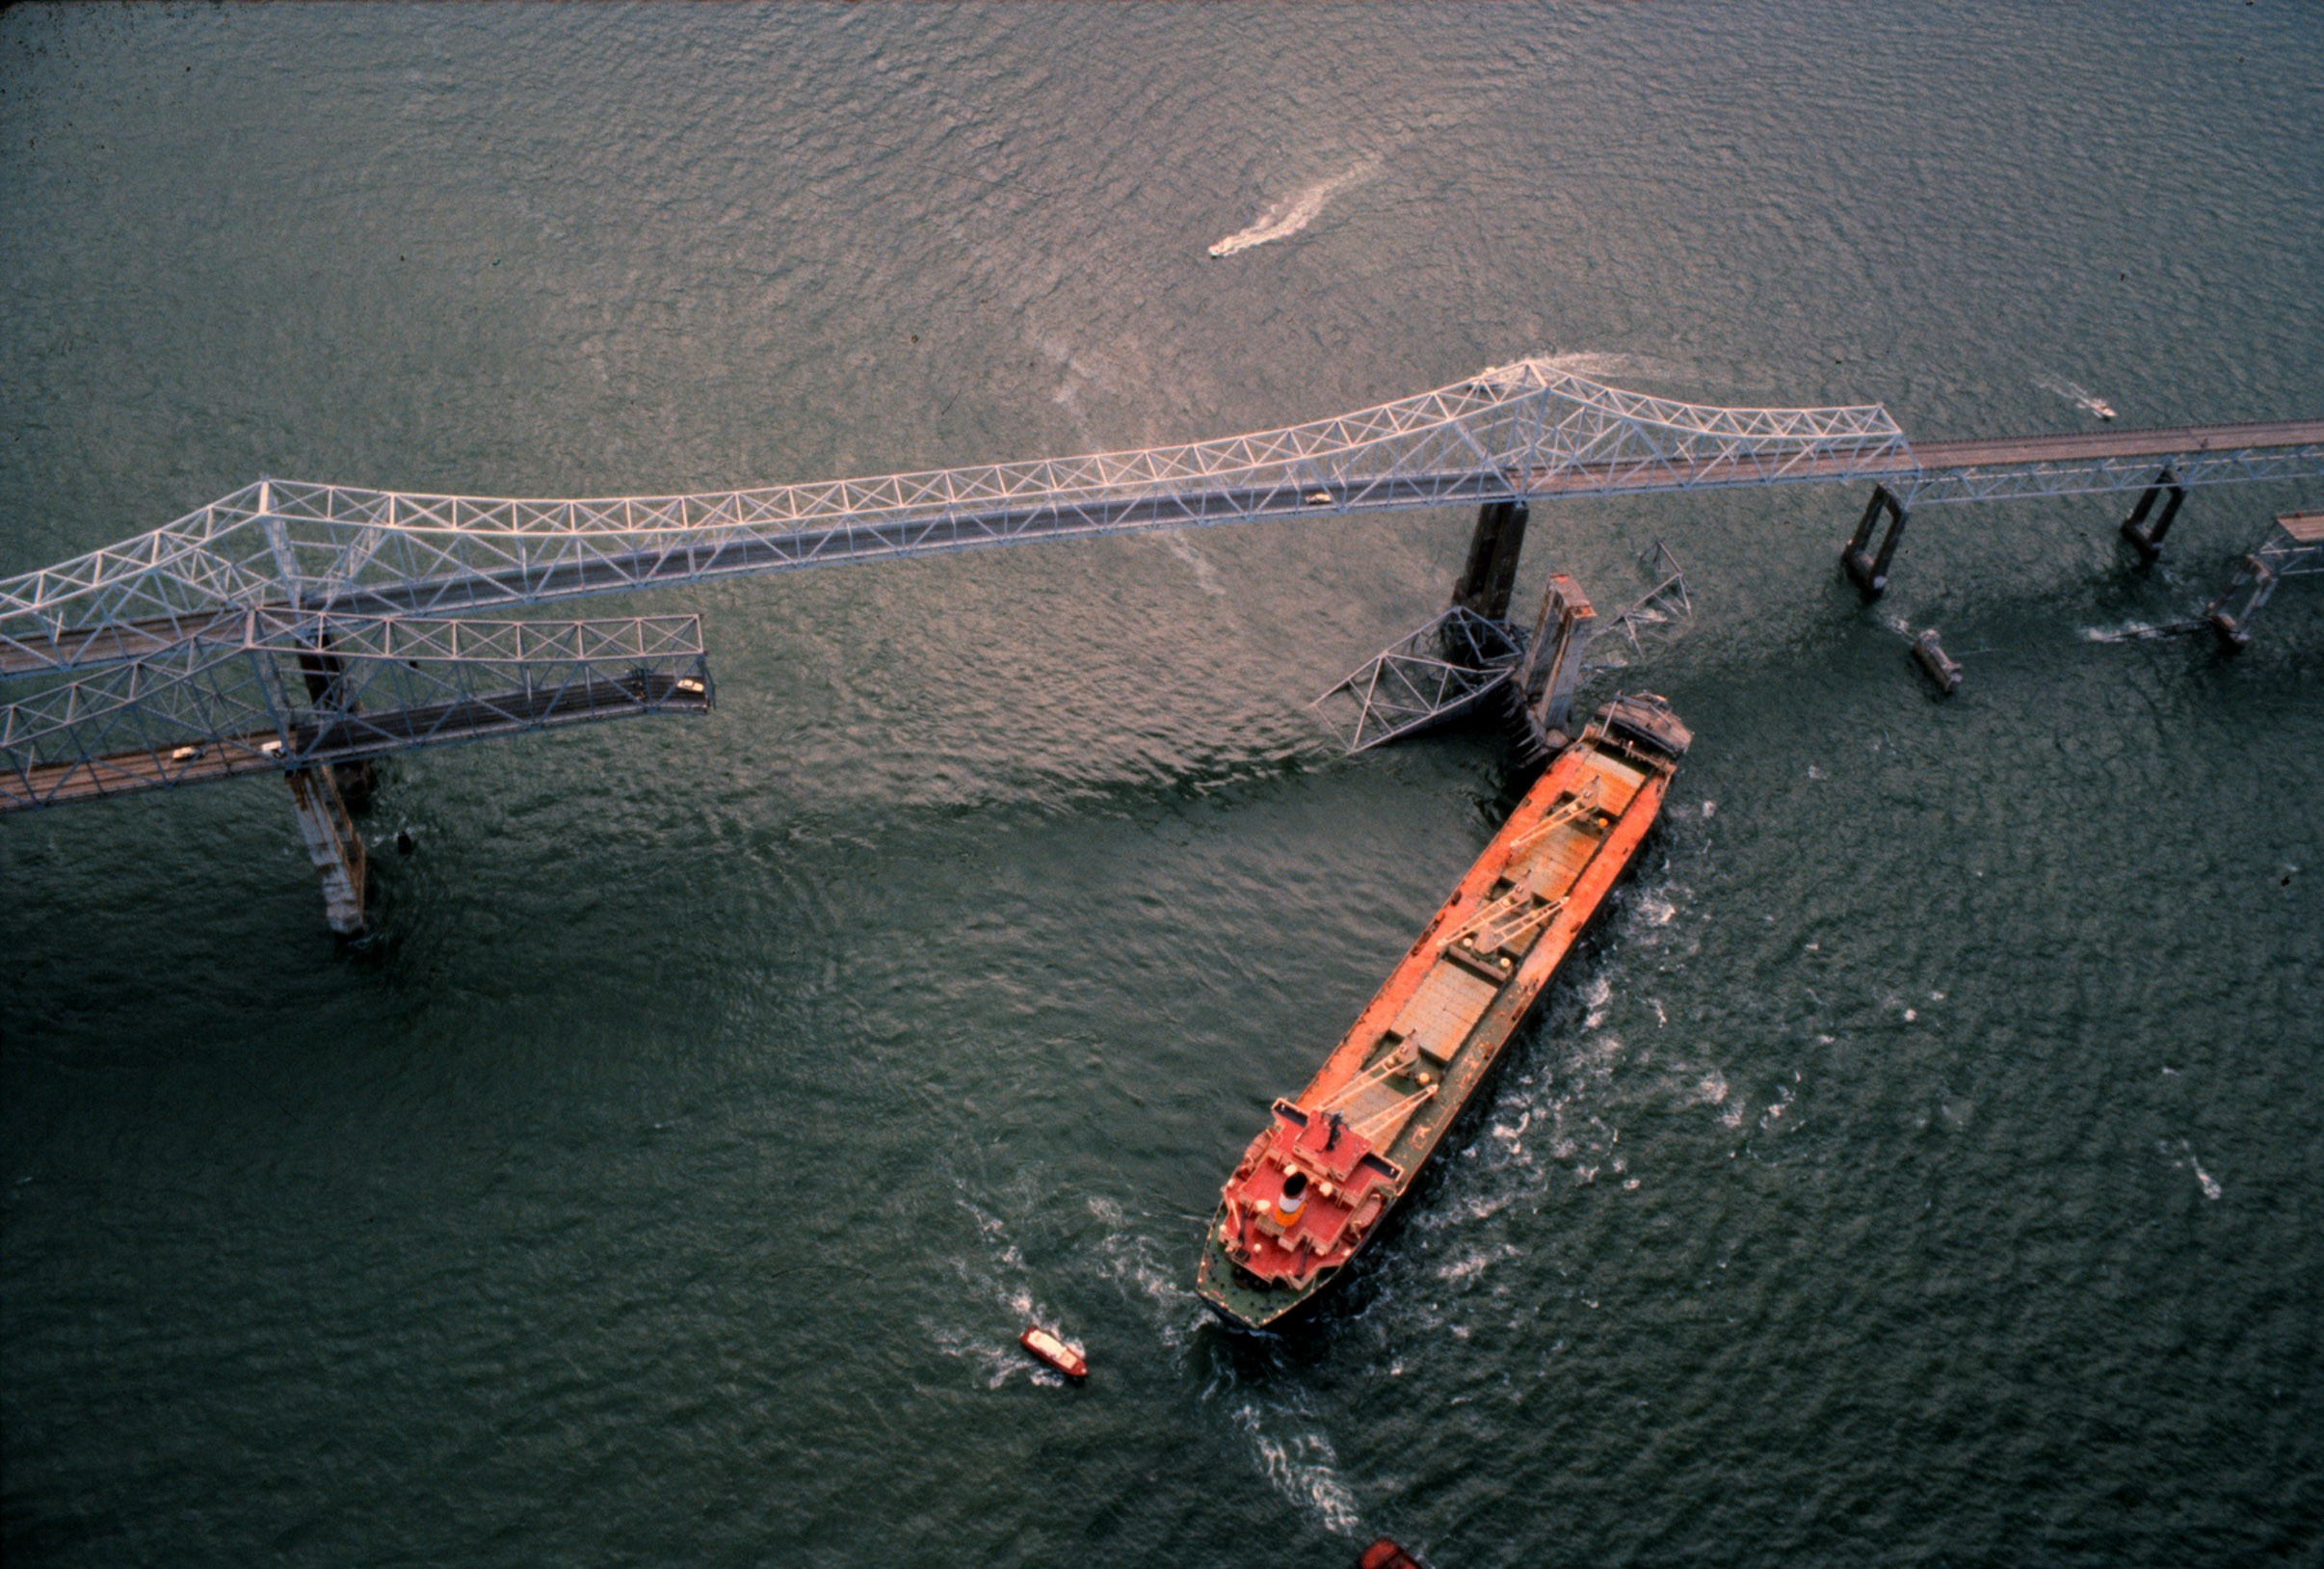
\includegraphics[width=0.8\linewidth]{ship-collision.jpg}
  \caption{阳光高架桥因船舶碰撞而倒塌}
  \label{fig:ship-collision}
\end{figure}

\subparagraph{Fire}
Fires, as extreme-event hazards for bridges, have a low probability of occurrence, but can cause significant
damage to affected bridge components including the deck, superstructure, and substructure, and can cause collapse of
entire spans. Although considered a low risk hazard, a recent study by the New York Department of Transportation
(DOT) in 2008 showed that nearly three times more bridges have collapsed because of fire than earthquakes (Kodur
et al. 2010).

Fires affecting bridges most typically occur due to vehicle accidents either on a bridge or on a roadway or
railway crossing below a bridge, but can also occur due to fires in adjacent buildings or facilities. Fires can vary in
intensity, the most intense due to accidents with tanker trucks or railroad tanker cars carrying large quantities of
highly flammable fuels or chemicals. The temperature of a recent fire below a bridge that was caused by a railroad
tanker car collision loaded with 30,000 gallons of Methyl Alcohol was estimated to be approximately 3000°F
(Stoddard 2002). Recent bridge fires involving tanker trucks carrying diesel fuel and gasoline were reported to have
reached temperatures over 2,000°F (Kodur et al. 2010).

The extreme high temperatures generated in these types of bridge fires for prolonged periods of time can significantly affect both steel and concrete structures. \cref{fig:tanker-truck-accident} shows examples of dramatic bridge fires caused by gasoline tanker truck accidents.

Steel bridge elements are especially vulnerable to high temperatures because of steel’s high thermal conductivity in which the temperature of unprotected steelwork will vary little from that of the fire. These cases can result in loss of strength, significant sagging, and possible collapse. Steel starts to loose strength at about 600° F, and its strength is reduced to about half its yield strength at about 1,100°F (Brandt et al. 2011). At about 1,700° F, the yield strength is only about 10\% or less. When fires at steel bridge elements reach these extreme temperatures, significant deformation and sagging usually occurs (if not total collapse) and the affected bridge elements will typically have to be replaced. \cref{fig:tanker-truck-collision} shows extreme sagging in a steel bridge span and heavy concrete pier deterioration after a gasoline tanker truck fire.

\begin{figure}
  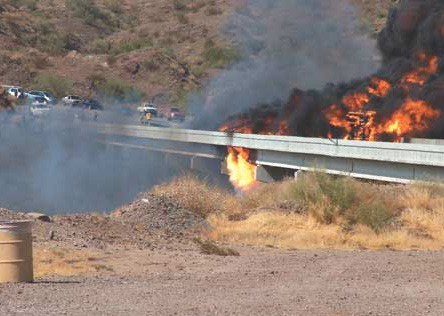
\includegraphics[width=0.6\linewidth]{tanker-truck-accident.jpg}
  % \caption{Intense bridge fire due to tanker truck accident. (Courtesy U.S. Fish and Wildlife Service)}
  \caption{油罐车事故导致桥梁大火}
  \label{fig:tanker-truck-accident}
\end{figure}
\begin{figure}
  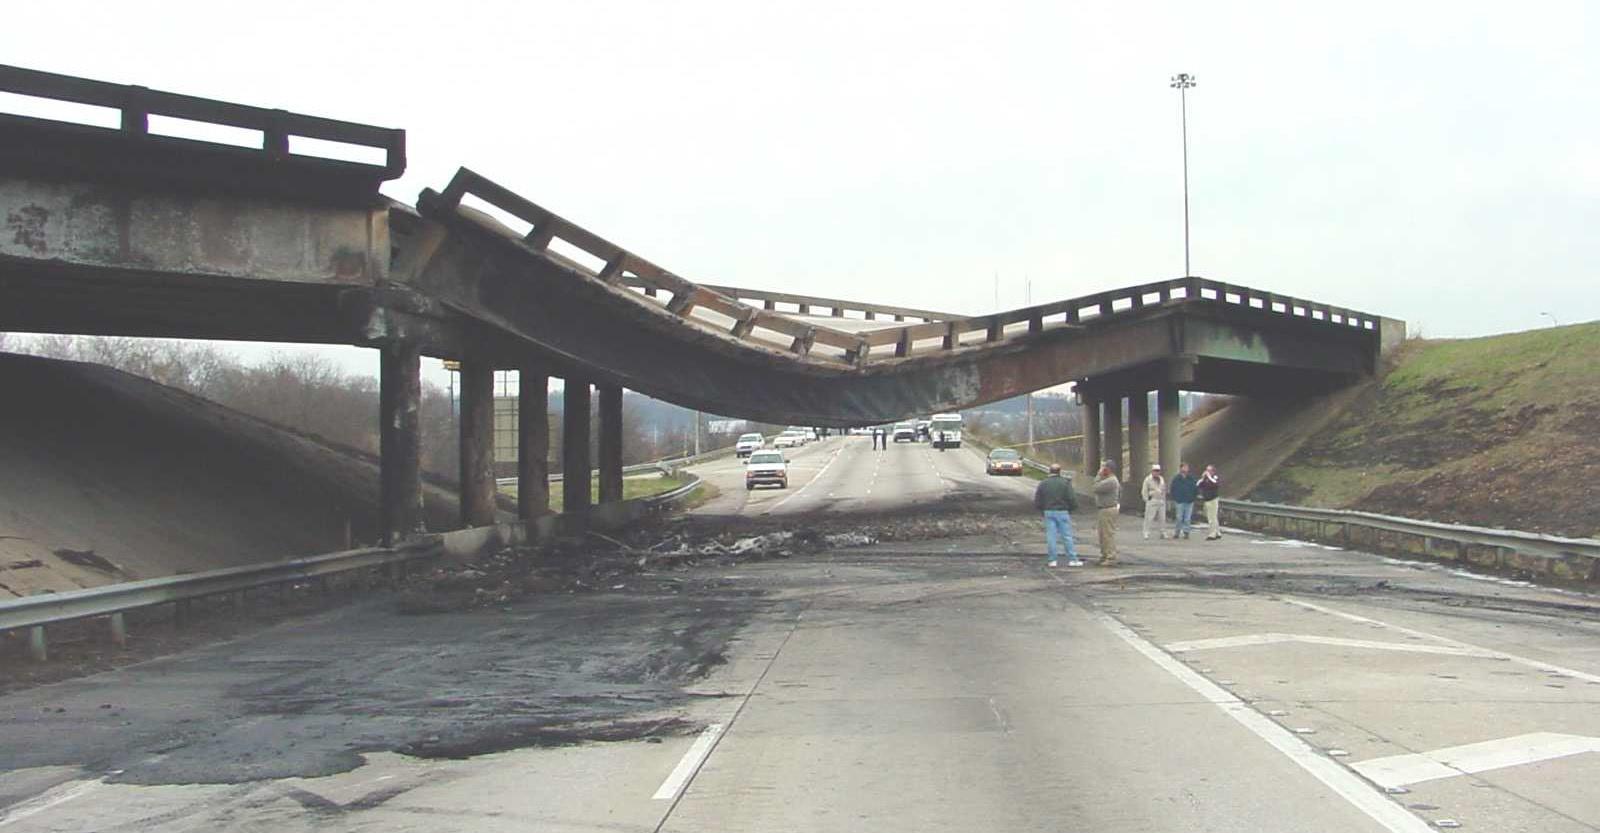
\includegraphics[width=0.8\linewidth]{tanker-truck-collision.jpg}
  % \caption{Steel bridge heavily damaged by fire after gasoline tanker truck collision. (Courtesy Alabama DOT)}
  \caption{钢桥在汽油罐车碰撞后被火灾严重损坏}
  \label{fig:tanker-truck-collision}
\end{figure}

In cases where damage to steel bridges sustained during a fire is not obvious (i.e., no clear signs of distress such
as sagging or buckling) the question is often raised as to whether permanent material property effects in heat affected
areas has occurred. It has been reported that steel will begin to encounter phase changes at temperatures greater than
1,300°F, whereby undesirable material properties such as reduced ductility and toughness can result during
uncontrolled cooling. The Pennsylvania DOT sponsored a study to examine the effects of fire damage on the
structural properties of steel bridge elements (Brandt et al. 2011). The study performed fire tests on painted steel
plate specimens at various temperatures up to 1,200°F and exposure times to evaluate changes in surface conditions
and discoloration and to then test for changes in material properties after cooling. The results showed that up to steel
surface temperatures of 1,200°F, the fire-exposed material after cooling still satisfied AASHTO material
specifications. They further concluded that if excessive distortions or deformations occurred, the steel would likely
have been subjected to steel temperatures well in excess of 1,200°F, and the corresponding sections would require
replacement.

Concrete bridge elements are typically able to withstand high temperatures with less distress than unprotected
steel elements. Concrete has inherent fire resistant properties due to its relatively low thermal conductivity, which
insulates interior portions of the member including reinforcement and/or prestressing steel from high surface
temperatures. Concrete does experience a reduction in strength and modulus of elasticity with high temperature.
Strength reduction is largely a function of type and size of aggregate. Concrete with siliceous aggregate (materials
consisting of silica and including granite and sandstone) begins to lose strength at about 800°F, and is reduced to about 55\% at 1200°F. Concrete containing light-weight aggregates (manufactured by heating shale, slate, or clay)
and carbonate aggregates (include limestone and dolomite) retain most of their compressive strength up to about
1200°F (Bilow and Kamara 2008). The following compares concrete temperature with typically encountered signs
of distress and concrete color (Shutt 2006).

\begin{itemize}
  \item Up to 200°F—little or no concrete damage;
  \item 500°F—surface crazing, localized cracks, iron bearing aggregates begin to acquire pink/red color;
  \item  700°F—cracks appear around aggregate, numerous micro cracks present in cement paste;
  \item  900°F—purple/gray color appears if enough iron and lime are present;
  \item  1,000°F—serious cracking of paste and aggregates occurs due to expansion. Purple/gray color may become
  more pronounced;
  \item  1,500°F—cement paste is completely dehydrated with severe shrinkage cracking and honeycombing.
  Concrete may begin to become friable and porous;
  \item  2,200°F—some components of concrete begin to fail; and
  \item  2,500°F—Concrete is completely failed.
\end{itemize}

In all cases, fire damaged structures should be evaluated as quickly as possible once the fire is extinguished to
determine the extent and severity of damage. Limits of concrete damage can often be tested with an impact-rebound
hammer. Concrete core samples can be taken for petrographic examination, which will determine the extent of
damage within the overall concrete matrix. Steel coupons can be taken to evaluate changes in material properties.

\subparagraph{Blast}

The possibility of terrorism against our nation’s bridges is an ever-increasing threat in today’s society. The risk
of blast attack is typically considered very low for most bridges, but major bridges or bridges along major corridors
that have high economic and/or socio-political impact can have greater risk. By their nature, bridges are very
accessible to vehicles carrying explosive devices traveling either on the bridge or below on crossed roadways. They are also susceptible to ships or boats carrying explosive devices below. Because bridges also vary in type and size,
the assessment of blast vulnerability can be very complicated. Until recently, there has been little work done or
information available concerning the effects of blasts on highway bridges or methods of analysis.

Extensive research is being undertaken by the FHWA (Duwadi and Munley 2011) to further understand the
behavior and effects of blast loadings on bridge elements. Part of these studies is also to develop methods for
evaluating risk and risk-mitigation strategies. The most significant research in the area of blast-resistant design
guidelines for highway bridges is being conducted under the NCHRP, project number NCHRP 12-72, which has been
recently documented in NCHRP Report 645 (Williamson et al. 2010). The response evaluation of reinforced
concrete bridge columns was a key part of this investigation. Other recent research reported by Agrawal and Yi,
2008, dealing with blast load effects on highway bridges developed computer models and showed through simulation
analysis that seismic capacities and blast-load effects are strongly correlated. Kiger et al. 2010, reported on bridge
vulnerability assessment and mitigation against explosions, and focused on response of posttensioned box girder
bridges under blast loads.

Blast loads are considered one of the extreme hazards affecting bridges, and even a small amount of explosive
can produce severe localized damage to a bridge element. In some cases, this localized damage can potentially
progress to global collapse of the structure (Kiger et al. 2010). There are a number of factors that affect the potential
damage to a bridge due to blast, including:

\begin{itemize}
  \item Size and type of explosive charge. Small explosive devices can have varied effects depending on placement
  and size of bridge element, but large truck bombs can be disastrous. The Oklahoma City Federal Building
  bombing in 1995 is an example of the devastating effect a large truck bomb.
  \item Proximity to blast—standoff distance. The distance from the blast to a bridge element is a critical parameter
  in determining the blast effect. For a given size blast, the effect will reduce significantly with relatively
  small increases in distance from the blast.

  Depending on the size and standoff distance, three blast categories exist: contact, close in, and plane wave
(Williamson et al. 2010). Contact blasts are very close and create high intensity, non-uniform loads where
breaching, or complete loss of material at a section in a bridge element, can occur. In this case, there can be extensive local destruction. A close in blast is farther away but still results in a localized spherical shock
wave striking the structure to produce a non-uniform load and impulse-dominated response. A plane wave
blast is far enough away to produce essentially planar shock waves and a uniform load on the structure. In
this case, the structure will be loaded in a manner that leads to global deformation, and will be resisted by the
entire structure or a number of combined elements.

\item Location of blast. Blasts can occur above or below deck. Above deck blasts can affect the deck itself, and
any structural elements above deck such as in a through truss, arch, or cable supported bridge. Blasts below
deck would typically have more effect on pier columns, but can affect superstructure if sufficiently large.
Below deck blasts can also have greater intensity because of the enclosed effect created by the overhead
structure, whereas above deck blasts have more freedom to dissipate without shock wave reflection.

\item Type and size of bridge element. Members with greater mass, hardness, and flexibility have greater blast resistance.
\item Structural redundancy. Having multiple load paths is a key factor in resisting overall structural collapse with any type of individual member failure. Multi-column piers or multi-girder superstructures are typically able to re-distribute internal forces and provide greater resistance to overall structure collapse.
\end{itemize}

A risk management approach can be taken for bridges with greater potential of fire or blast hazard. These
bridges can be identified by reviewing major corridors that would experience the greatest economical and sociopolitical
impact if damaged by these extreme event hazards. Potential mitigation including local protective measures,
alternative routes, or accelerated reconstruction strategies can be evaluated for these higher-risk bridges.

% \subparagraph{Seismic}
\subparagraph{地震}
\label{subpar:seismic}

Earthquakes, including those of moderate intensity, are extreme hazard events that can cause significant damage
to bridges, and particularly to existing bridges that were designed under older codes and have not been retrofitted.

The 1971 San Fernando earthquake in California, which resulted in numerous bridge collapses, has often been
cited as a watershed event in bridge engineering since it demonstrated the inadequacy of seismic bridge design practices of the time (Buckle et al. 2006). The FHWA became a major sponsor of bridge seismic research shortly
afterward, including research on retrofitting existing bridges.

Other subsequent major California seismic events such as the 1989 Loma Prieta and 1994 Northridge
earthquakes, and the 1995 Kobe, Japan earthquake caused significant bridge damage and collapse, which also led to
further research and understanding of bridge seismic behavior (Azizinamini and Ghosh 1997).

The observed damage and knowledge gained from these previous events, along with extensive research
undertaken since 1971, have led to significantly improved seismic bridge design specifications (AASHTO Guide
Specifications for LRFD Seismic Bridge Design, 2nd Edition, 2011 and AASHTO LRFD Bridge Design Specifications,
6th Edition, 2012), advanced concepts for seismic retrofit (Seismic Retrofitting Manual for Highway Structures: Part
1—Bridges, Buckle et al. 2006), and guidance for seismic design of foundations (LRFD Seismic Analysis and Design
of Transportation Geotechnical Features and Structural Foundations, Kavazanjian et al. 2011).

The current approach adopted in the LRFD Specifications (2012) is to design new conventional (or ordinary)
bridges for a design earthquake, or level of ground motion, that represents the largest motion that can be reasonably
expected during the life of the bridge. It implies that ground motions larger than the design earthquake could occur
during the life of the bridge, but their likelihood of happening is small. This likelihood is usually expressed as the
probability of exceedance, and it may also be described by a return period in years. The specifications call for a
design earthquake that has a 7\% probability of exceedance in 75 years (approximately 1000 year return period).
Bridges designed and detailed under these provisions may suffer damage but should have low probability of collapse.
Key principles used for the development of these specifications are that small to moderate earthquakes should be
resisted within the elastic range of the structural components without significant damage, and that large earthquakes
should not cause collapse of all or part of the bridge, although they may cause significant damage requiring
replacement.

One of the key considerations in seismic design is repairability of the damage to bridges during moderate seismic
events. Oftentimes the so-called “minor damage” may require complete replacement of the bridge. In the case of the
1995 Hyogoken-Nanbu earthquake in Kobe, Japan (Bruneau et al. 1996; Chung 1996; Shinozuka et al. 1995;
Azizinamini and Ghosh 1997) steel bridges suffered damages to superstructure elements including inadequate crossframe
detailing leading to lateral bending of the girder webs near girder ends. This resulted in major retrofit activities and the closing of major highways, such as the Hanshine Expressway, which was closed for more than a year. The
Kobe experience demonstrated that even “minor damage” to steel bridges during seismic events can result in damage
that could be very difficult to repair. Among the lessons learned is that critical elements of the bridge that are difficult
to inspect and repair must be protected from any level of damage and remain elastic during the entire seismic
excitation.

Service life design philosophy needs to be considered when following seismic design principles, by examining
the effects of repair on traffic interruption after small to moderate earthquakes. In particular, the areas with potential
to form plastic hinges, as described below, must be detailed so that the repair can proceed with little or no
interruption to traffic. The major areas of concern are substructure elements where most plastic hinges are
anticipated. The superstructure elements of the bridge are mainly kept elastic during entire seismic event.

Seismic load behavior is largely un-known; therefore, the design philosophy for buildings and bridges is to work on behavior of the structure under known conditions. Specifically, the design objective is to predefine the damage locations and design them accordingly by providing adequate levels of ductility. In the case of bridges, the preferred damage locations are at the ends of pier columns (formation of plastic hinges). In the direction of traffic, it is preferred to put columns in double curvature as shown in \cref{fig:deflected-shape-longtitudinal}. This allows larger portions of the pier column (two plastic hinges vs. one for single curvature) to participate in energy dissipation.

\begin{figure}
  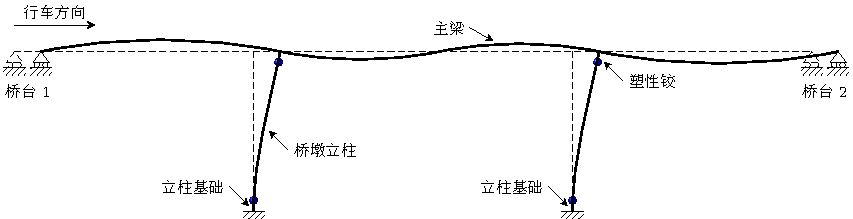
\includegraphics{deflected-shape-longtitudinal.pdf}
  % \caption{Deflected shape of a 3-span bridge under longitudinal (along traffic) direction.}
  \caption{三跨桥纵向(沿行车方向)变形形状}
  \label{fig:deflected-shape-longtitudinal}
\end{figure}

In the transverse direction, pier columns are usually designed to act in single curvature, as shown in \cref{fig:deflected-shape-longtitudinal-transverse}.

\begin{figure}
  \begin{minipage}{0.45\linewidth}\centering
  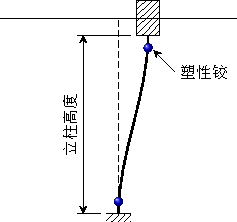
\includegraphics{deflected-pier-longtitudinal.pdf} 
    \subcaption{纵桥向变形}
  \end{minipage}
  \begin{minipage}{0.45\linewidth}\centering
  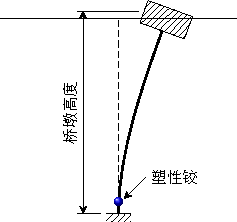
\includegraphics{deflected-pier-transverse.pdf}
    \subcaption{横桥向变形}
  \end{minipage}
  % \caption{Deflected shape of pier column in longitudinal and transverse directions.}
  \caption{桥墩立柱在纵、横桥向的变形}
  \label{fig:deflected-shape-longtitudinal-transverse}
\end{figure}

Under longitudinal excitation, plastic hinges are located near the top and bottom of the columns, while under transverse excitation; the plastic hinge is located near the bottom of the pier column.

The main design feature in seismic design of bridges is to keep the superstructure elements completely elastic during an entire seismic event. Repairing any elements of the superstructure, even “minor” damage, could be very time consuming and result in a major interruption to traffic. The elements that should remain elastic are referred to as protected elements in capacity design approach. The inelasticity is then forced to take place at predefined locations within the substructure. The predefined damage locations are the weak links or fuses that control the level of forces to be transmitted to superstructure elements. This design approach is referred to as the capacity design approach and is routinely used for designing bridges in seismic regions.

In the capacity design approach, protected elements are designed for the largest possible force effects they might
experience, considering the over-strength that may exist because of higher actual material strength than that specified
in design.

Areas with Seismic Risk

While earthquakes are sometimes considered primarily a California or West Coast problem in the continental
United States, data produced by the United States Geological Survey (USGS) National Seismic Hazard Mapping
indicates that at least 40\% of the United States is subject to damaging, ground shaking levels (Kavazanjian et al.
2011). Since 1996, the USGS has developed and updated maps that have depicted areas in the United States with various levels of seismic risk. These maps display earthquake ground motions for various risk levels including 2\%,
5\%, and 10\% probability of being exceeded in 50 years. \cref{fig:seismic-hazard-map} shows the USGS seismic hazard map depicting
peak ground acceleration (PGA) levels with a 2\% probability of being exceeded in 50 years, or a return period of
approximately 2500 years. Along with areas along the west coast, these maps further show areas of high seismic risk
in the central and eastern United States.

\begin{figure}
  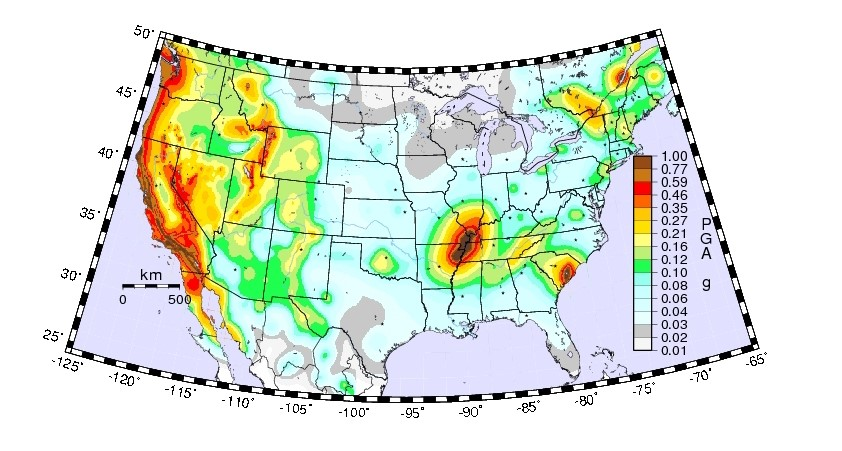
\includegraphics[width=\linewidth]{seismic-hazard-map.jpg}
  % \caption{Seismic hazard map, PGA, 2\% in 50 years. (Courtesy U.S. Geological Survey)}
  \caption{地震风险区划图(\acrfull*{pga} 超越概率 50 年 2\%) }
  \label{fig:seismic-hazard-map}
\end{figure}

Performance During Earthquakes

Moehle and Eberhard, 2000, discuss various causes and types of damage that bridges experience during
earthquakes. Key factors that affect the type and severity of bridge damage include:

\begin{itemize}
  \item Close proximity to fault rupture. This results in ground motions having high horizontal and vertical ground accelerations as well as large velocity pulses.
  \item Soil conditions. Soft soil sites can significantly amplify ground motion. Soil liquefaction and lateral spreading results in permanent substructure deformations and loss of superstructure support.
  \item Structural Configuration. Bridges are most vulnerable that have excessive deformation demands in rigid,
  nonductile elements; complex or non-uniform structural configuration; curved or skewed configuration; or non redundancy..
\end{itemize}

Major types of damage include:

\begin{itemize}
  \item Unseating at joints. Superstructure expansion joints introduce a structural irregularity that can have
  catastrophic consequences. These joints can occur within a span or at substructure supports. Irregular ground
  shaking can induce superstructure movements that can cause a span to unseat. Unrestrained superstructures
  can be toppled from their supporting substructures due to shaking or differential support movement
  associated with ground motion. Bridges with short seats are especially vulnerable. Use of restrainers has
  been effective in minimizing this risk. \cref{fig:Loma-Prieta-earthquake-damage} shows a span unseating failure on the Oakland Bay Bridge
  in San Francisco during the Loma Prieta Earthquake in 1989.
  \item Superstructure damage. Superstructures typically have sufficient strength to remain elastic during
  earthquakes, and are unlikely to be the primary cause of collapse of a span. However, certain types of
  superstructure damage have been observed, including bearing damage, pounding of adjacent units at
  expansion joints, and transverse bracing or diaphragm damage.
  \item Substructure damage. Substructures typically sustain the most damage, and can be categorized by column
  failure and abutment damage.
  \begin{itemize}
    \item Column failure. The lateral load capacity of a pier is limited by the shear or flexural strength of its
    columns. For non-ductile reinforced concrete columns, shear failure is often the primary mode of failure
    when subject to large inelastic demands during strong earthquakes. Column failure is often the primary
    cause of bridge collapse during earthquakes (Moehle and Eberhard 2000).

    Most damage to columns can be attributed to inadequate detailing, which limits the ability of the column
to deform inelastically. In concrete columns, detailing inadequacies can produce flexural, shear, splice,
or anchorage failures. In steel columns, local buckling has been observed to lead progressively to
collapse (Moehle and Eberhard 2000). \cref{fig:Loma-Prieta-earthquake-damage} shows a non-ductile column shear failure on the Cyprus Street Viaduct in San Francisco that
occurred during the Loma Prieta Earthquake in 1989.
    \item Abutment damage. Damage to shear keys and wing walls is often prevalent.
  \end{itemize}
\end{itemize}

\begin{figure}
  \begin{minipage}{0.55\linewidth}\centering
    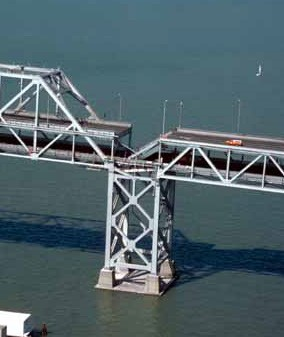
\includegraphics[height=8cm]{lomaprieta1.jpg}
    % \subcaption{Oakland Bay Bridge upper roadway span unseating and    collapse.}
    \subcaption{奥克兰海湾大桥上部车行道跨度脱落和倒塌}
  \end{minipage}%
  \begin{minipage}{0.45\linewidth}\centering
    \includegraphics[height=8cm]{lomaprieta2.jpg}
    % \subcaption{Cyprus Street viaduct support column collapse}
    \subcaption{Cyprus 高架桥支撑柱倒塌}
  \end{minipage}
  % \caption{1989 Loma Prieta earthquake damage near San Francisco, California. (Courtesy U.S. Geological Survey)}
  \caption{1989 年加利福尼亚州旧金山附近的 Loma Prieta 地震造成的破坏}
  \label{fig:Loma-Prieta-earthquake-damage}
\end{figure}

\subsubsection{Reduced Service Life due to Production/Operation Defects}

Decisions made for the production of bridges and activities during its operation can have a significant influence
on overall bridge service life. These production and operation influences are introduced in the fault tree provided in
\cref{fig:production-operation-defects}, and include decisions made during the design and detailing of the bridge, quality of fabrication and /or
manufacturing, quality of construction, the level of inspection performed during operations, and the level and quality
of maintenance. Each of these categories can be further developed to identify the lowest or basic levels causing
deficiency, but these lower levels can vary significantly for each bridge system, component, or element type. The
discussion here will address general issues that are common to all.


\begin{figure}
  % \includegraphics[width=\linewidth]{graphic-file}
  \caption{Production or operation defects}
  \label{fig:production-operation-defects}
\end{figure}

\paragraph{Design/Detailing}
Decisions made during the system selection, design, and detailing phase of a bridge project can significantly
impact the service life of the bridge. It is incumbent upon designers to understand the implications of these decisions
in order to help in making rational choices that will improve service life.

Examples of design/detail issues causing reduced service life include:
\begin{itemize}
  \item Using bridge systems with deck joints that can ultimately leak and cause service life issues below. See
  \cref{chp:jointless-bridge} on jointless bridges.
  \item Providing inadequate drainage systems that allow moisture to remain on bridge decks, leading to
  deterioration, or improper layout, capacity, or slopes on drainage elements that ultimately lead to clogging
  and malfunction.
  \item Dealing with moisture trap details on steel bridges that hold water and debris resulting in coating damage and
  steel corrosion. See \cref{chp:corrosion-prevention-steel-bridge} on corrosion protection of steel bridges
  \item Using fatigue-prone details.
  \item Considering design errors. Effective quality assurance (QA) and quality control (QC) in design process is
  necessary to avoid errors.
\end{itemize}

\paragraph{Fabrication/Manufacturing}
Defects in fabrication or manufacturing can lead to reduced service life in steel or concrete bridge elements.
Undetected fabrication defects can lead to fatigue damage in steel structures.

\paragraph{Construction}
Defects or damage in construction can reduce service life in steel or concrete bridge elements. Poor concrete
placement and curing practices can have significant effects. See \cref{chp:materials} on material and \cref{chp:bridge-decks} on decks for
further discussion on concrete placement.

Transportation and erection of both steel and concrete girders can become an issue if not handled properly. As
high-performance materials are increasingly used for bridge construction (HPS and/or HPC), girders tend to become
longer and their webs slimmer. Transportation of these girders can then cause higher stresses or out-of-plane
bending, which can result in cracking. Girder stability during erection, particularly in curved steel girders, needs to
be carefully addressed.


\paragraph{Inspection}
Proper inspection during bridge operation is essential to identify defects and issues early, before more serious
conditions develop.

\paragraph{Maintenance}
Lack of or inadequate maintenance can allow deterioration to initiate throughout the bridge system and develop
into serious conditions whereby the only alternative is costly component or element replacement. Applying the
appropriate bridge preservation treatments and activities at the appropriate time can extend bridge service life at a
lower lifetime cost (FHWA 2011).

FHWA publication FHWA-HIF-11042 (FHWA 2011) provides general guidance on the importance and benefits
of preventive maintenance as part of an overall bridge preservation program. Examples of various cost-effective
preventive maintenance activities that can be applied to decks, superstructure, and substructure components are
further discussed in Section 2.4.1.3.

\subsection{Factors Affecting Service Life of Deck Componet}\label{subsec:factors-affect-deck}
The deck component includes several elements as described in Section 2.2.2.

\begin{description}
  \item [Bridge deck] service life and the factors affecting service life are described in detail in \cref{chp:bridge-decks}. Concrete
  bridge decks are particularly affected by thermal and coastal environments in which chloride penetration can cause
  reinforcing steel corrosion leading to concrete cracking and spalling. This cracking can cause the concrete
  surrounding the steel reinforcement to reach the corrosion threshold limit in environments where the top of the bridge
  deck is exposed to chlorides, such as deicing salts. Other concrete deck issues include wear and freeze/thaw damage.
  \item [Bridge expansion devices] commonly referred to as bridge joints, are discussed in \cref{chp:expansion-devices}.
  \item [Drainage systems] are most affected by lack of maintenance that causes clogging and malfunction.
  \item [Bridge railings] are affected by wet chloride environments that cause corrosion of reinforcing steel and concrete
  cracking and spalling in concrete railings. This condition is exacerbated at cold joints between the concrete barrier
  and top of slab, where salt moisture can easily penetrate and cause reinforcing corrosion. The same environments
  cause corrosion of steel railings.
\end{description}

\subsection{Factors Affecting Service Life of Supersturcture Componet}
\subsubsection{Steel Superstructures}
\paragraph{Load-Induced Deficiency—Fatigue and Fracture}
Early-welded steel structures have a history of cracking at certain types of weld details due to load-induced and
distortion-induced fatigue. Cracking at I-beam cover plate terminations or at other longitudinal weld terminations in
tension zones has been particularly evident. Cracking in girder webs due to out-of-plane bending within stiffener web
gap regions next to cross frame attachments also became a common problem. Subsequently, extensive research and
laboratory testing has provided an understanding of fatigue behavior, and different weld detail types were found to
have varying levels of fatigue susceptibility. Newer design provisions and recommended details were developed that
provide solutions for both load-induced and distortion-induced fatigue that will achieve desired service life.


Steel bridges can fail by fracture, which is the rapid, unstable propagation of a larger flaw, most likely the result
of fatigue. Fatigue crack initiation is independent of steel type and strength, but possible brittle fracture is influenced by steel toughness among other variables. Early steels were more susceptible to brittle fracture, but in recent years,
new high-performance steels—HPS 50W, 70W, and 100W—have been developed with very high toughness
characteristics. Although somewhat more costly than conventional-grade steels, high-performance steels are now
encouraged where applicable, particularly in non-redundant or fracture-critical applications. Use of high-performance
steel allows time for any fatigue cracks that may have developed to be found during regular bridge safety inspections
before fracture can occur.

Fatigue should not be an issue in new steel bridges designed in accordance with the latest LRFD Specifications.
Extensive research has been done in recent years to identify causes and solutions for fatigue- and fracture-related
problems. When using proper details and fabrication methods, both load-induced and distortion-induced fatigue
problems should not be an issue in achieving desired service life.

\paragraph{Deficiency Due to Natural or Man-Made Hazards—Corrosion}
Corrosion is a fundamental limitation of steel as a construction material, and is the result of exposure to oxygen
and moisture. The process is greatly accelerated in the presence of chloride ions from roadway deicing salt or salt
spray in a marine environment. Deck drainage with deicing salt leaking through open deck joints is a leading cause of
steel element corrosion in bridges.

Corrosion control should be designed into the overall steel bridge system. Use of systems that eliminate or
minimize deck joints will have a significant effect in reducing corrosion. Details that serve to protect and keep the
steel dry should be included in the design. Among these are bridge system solutions that eliminate deck joints,
preventing salt-contaminated drainage from reaching steel elements below.

Salt marine environments or locations subject to deicing salt spray from below also create harsh environmental
conditions subject to corrosion; thorough cleaning and zinc-rich primer coating systems can provide long-term
protection. However, requirements for related long-term coating maintenance cannot be overlooked, and must also be
designed into an overall corrosion protection plan.

To achieve long-term bridge durability, a corrosion resistance plan must be a design requirement for every new
or rehabilitated steel structure. This plan should include the use of “best painting practices” and a maintenance plan
that addresses painting priorities and timetables.

Best painting practices now include paint systems that contain metallic zinc as the corrosion-resistant pigment.
Zinc coatings provide “galvanic protection” to the steel, in which zinc (the more noble metal) will oxidize (corrode)
in preference to the steel. To protect the zinc-coating layer from oxidation, additional coating layers are applied over
the zinc-rich primer.

There are many studies that demonstrate the value of zinc coatings as a steel protection system. In addition to
zinc-rich paint, these zinc coatings also include galvanizing and metalizing. Their use should be considered carefully
as part of the best plan for achieving extended service life.

Weathering steel has also found widespread use in steel bridges, and has been used in both unpainted and painted
applications. Weathering steel is corrosion resistant in some circumstances, but it is adversely affected by continual
drainage and roadway salts, particularly below joints. Typically, special coatings are applied in these locations when
using weathering steel.

In addition to weathering steel, a new structural stainless steel for bridges, ASTM A1010, has been developed for
use in severe corrosive environments.

\subsubsection{Concrete superstructures}
\paragraph{General Deficiencies}
There are numerous causes of deterioration in concrete superstructure elements. \cref{chp:materials} on materials discusses
the various factors influencing durability of concrete. Typically, the deficiencies are due to three main factors that
were described in the fault tree analysis in Section 2.3.1. These are:
\begin{itemize}
  \item Load-Induced:
  \begin{itemize}
    \item Traffic causing vibration, impact, or wear; and
    \item Restrained thermal movement causing internal stress and cracking.
  \end{itemize}
  \item Natural or Man-Made Hazards:
  \begin{itemize}
    \item Environmental influences including effects from moisture and freezing and thawing, and reinforcing
    corrosion due to chloride exposure; and
    \item Chemical influences including exposure sulfates, carbon dioxide, alkalis, and various acids.
  \end{itemize}
  \item Defects in production/operation, primarily defective placement, curing and maintenance.
\end{itemize}
The degree and severity of concrete deterioration depends on the level of load and environmental influences to which the bridge is subjected.

The durability of concrete exposed to these influences is highly dependent on design practice, materials, and their proportioning and workmanship during construction. While all of these influences are important, the principal deterioration of concrete elements is the corrosion of steel reinforcement, which results in severe cracking, spalling, and delamination of the surrounding concrete. Cracking of the concrete often compromises the protection provided by the depassivated zone around the steel reinforcement.

Concrete superstructures in thermal or marine environments are not exposed to the same concentration of chlorides as the top of a bridge deck that may be directly in contact with deicing salts. They are, however, susceptible to the same type of corrosion, only at a slower rate through the same mechanism of failure.

\paragraph{Adjacent Box Beam Deterioration}
Bridges constructed using adjacent box beams have been in service for many years and have generally performed well. However, a recurring problem with non-composite beams is cracking in the grouted joints between adjacent units, resulting in reflective cracks in the wearing surface. The development of these longitudinal cracks jeopardizes the durability and structural behavior of adjacent box beam bridges. In most cases, the cracking leads to leakage, which allows chloride-laden water to penetrate the sides and bottom of the beams and cause corrosion of the non-prestressed and prestressed reinforcement, see \cref{fig:longitudinal-cracking-adjacent-box-beam}. In addition, the load distribution among the beams is adversely affected, requiring the loaded beams to carry more load than originally intended.

\begin{figure}
  \begin{minipage}{0.5\linewidth}\centering
    \includegraphics[height=5.2cm]{adjacentbox1.jpg}
    \subcaption{梁底开裂}
  \end{minipage}%
  \begin{minipage}{0.5\linewidth}\centering
    \includegraphics[height=5.2cm]{adjacentbox2.jpg}
    \subcaption{路面反射裂缝}
  \end{minipage}
  % \caption{Longitudinal cracking in adjacent box beam bridge. (Courtesy HDR)}
  \caption{\gls*{adjacentbox}桥纵向开裂}
  \label{fig:longitudinal-cracking-adjacent-box-beam}
\end{figure}

Ultimately, these conditions have led to severe beam deterioration and failure causing premature replacement of entire bridges. On December 27, 2005, the east-side fascia beam of the Lakeview Drive Bridge over I-70 in Washington, Pennsylvania failed near mid-span and fell to the highway below, as shown in \cref{fig:failure-adjacent-box-beam}. Inspection of the bridge revealed heavy spalling and corrosion of the strands on the bottom flange of the failed non-composite prestressed concrete box beam. Additional corrosion was revealed on other box beams and the bridge was subsequently removed from service.

\begin{figure}
  \includegraphics[width=0.7\linewidth]{failure-adjacent-box.jpg}
  % \caption{Failure of adjacent box beam bridge in Pennsylvania. (Courtesy Pennsylvania DOT)}
  \caption{宾夕法尼亚州\gls*{adjacentbox}桥失效}
  \label{fig:failure-adjacent-box-beam}
\end{figure}

\subsection{Factors Affecting Service Life of Substructure Componet}
There are numerous causes of substructure deterioration, which can be categorized in three areas:
\begin{itemize}
  \item Improper detailing and improper consideration of appropriate forces due to applied mean recurrence level event forces, such as scour, vessel collision and earthquake;
  \item Deterioration caused by corrosion and section loss, primarily from chloride intrusion; and
  \item Seized bearings and unintended movement restraint.
\end{itemize}

\subsubsection{Mean Recurrence Level Event Forces}
As bridge service life increases, bridges are subjected to environmental conditions for a longer period of time. Many of these conditions are accounted for in design by the use of traditional recurrence values of extreme environmental conditions such as those for hydraulic stages, wind loads, and seismic events. Design for vessel impact is treated similarly. The increased service life from 50-year (pre-LRFD) to 75-year (LRFD) to 100-year service life increases the statistical probability of exceeding the design recurrence level event.

The importance of considering these events has been exemplified by numerous bridge incidents, including, but not limited to:
\begin{itemize}
  \item The 1987 collapse of the I-90 Bridge over Schoharie Creek emphasizing the importance of providing adequate hydraulic openings and flow characteristics under bridges. Undermining of embankments, such as
  shown in \cref{fig:scour-undermining-abutment}, and undermining of pier foundations due to scour remain primary causes of bridge
  failures around the nation.
  \begin{figure}
    \includegraphics[height=4.8cm]{scour1.jpg}\hfill
    \includegraphics[height=4.8cm]{scour2.jpg}
    % \caption{Scour undermining of bridge abutment. (Courtesy Atkins North America, Inc.)}
    \caption{冲刷导致桥台破坏}
    \label{fig:scour-undermining-abutment}
  \end{figure}
  \item  Multiple catastrophic vessel and bridge accidents around the world from the 1960s to the mid-1980s (Knott and Larsen 1990), including the 1964 and 1974 collapses of the Pontchartrain Bridge in Louisiana and the 1980 collapse of the Sunshine Skyway Bridge in Florida
  \item Impact forces from motor vehicles, similar to vessel collision, and subsequent fires that have resulted in structural damage to substructure units. Susceptibility to damage from these aberrant vehicle impacts
  underscores the importance of pier protection.
  \item The 1971 San Fernando Earthquake, and subsequent major earthquakes identified in \cref{subpar:seismic}, which caused catastrophic damage to numerous bridges and stimulated research relating to bridge performance during seismic events \cite{aashto1983s}.
\end{itemize}

\subsubsection{Substructure Deterioration due to Material Deterioration, Corrosion, and Section Loss}
Corrosion deterioration in substructure elements is due to numerous causes, including:
\begin{itemize}
  \item Chloride intrusion due to leakage of expansion joints and bridge drainage where deicing salts are utilized to remove snow and ice from bridge decks,
  \item Chloride intrusion due to direct salt splash from traffic travelling on roadways below the bridge where deicing salts are utilized to remove snow and ice from the pavement,
  \item Chloride intrusion found in marine and brackish water environments affecting exposed elements such as  those shown in \cref{fig:marine-pile-degradation}, and
  \begin{figure}
    \includegraphics[height=8cm]{marine-pile1.jpg}\hfill
    \includegraphics[height=8cm]{marine-pile2.jpg}
    % \caption{Marine pile degradation—jacket failure on concrete pile and corroded steel pile. (Courtesy Atkins North America, Inc.)}
    \caption{海洋环境桩基退化——混凝土桩和腐蚀的钢桩上的导管架失效。}
    \label{fig:marine-pile-degradation}
  \end{figure}
  \item  Corrosion due to concrete cracking induced by alkali-silica reaction (ASR) and other concrete quality issues.
\end{itemize}

Many of the issues affecting durability of the substructure are similar to the issues affecting the bridge in general.
Leakage of expansion joints and bridge drainage creates a major problem for the superstructure and substructure
below the leak. Strategies to address the causes and possible relief of these leaks are addressed in \cref{chp:expansion-devices} on joints.
Strategies to address concrete quality issues, such as ASR and others, are addressed in \cref{chp:materials} of this Guide. This
section of the chapter addresses issues related to substructure in a marine environment or in grade separations where
deicing salts can be splashed on supporting members.

Degradation of concrete and steel structures in aggressive corrosive environments, such as the splash zone in a
marine environment, has historically led to a reduction in service life of numerous structures. The areas particularly
susceptible to chloride intrusion are the splash zone, areas of poor concrete consolidation, spalls, and pile splices.

The degradation of piles and other deep foundation elements in marine environments has spawned an enormous concrete and steel protection and repair industry, which has developed numerous products dealing with the preservation of these deteriorating structural elements (Heffron 2007). Many of these products are relatively new, and their long-term effectiveness and expected life are not verifiable with historic data. Some of the more promising techniques include:

\begin{itemize}
  \item Cathodic protection with embedded sacrificial anodes;
  \item Pile jacketing, as shown in \cref{fig:pile-restoration-pile-encapsulation};
  \item Metalized coatings;
  \item Crystalline admixtures for crack sealing;
  \item Repassivation through the removal of chloride ions; and
  \item Various combinations of the these techniques.
\end{itemize}

\begin{figure}
  \includegraphics[height=5.5cm]{pile-restoration1.jpg}\hfill
  \includegraphics[height=5.5cm]{pile-restoration2.jpg}
  % \caption{Pile restoration with pile encapsulation and epoxy grout fill. (Courtesy Atkins North America, Inc.)}
  \caption{通过桩包封和环氧灌浆填充进行桩基修复}
  \label{fig:pile-restoration-pile-encapsulation}
\end{figure}

\subsubsection{Potential Effect of Climate Change and Service Life of Bridges in Coastal Areas}

Climate-related impacts that require adaptation are already being observed in the United States and its coastal waters (USGCRP 2009) and empirical evidence suggests that many of these and other impacts will grow in severity in the future (USGCRP 2009). Sea level has increased along most of the U.S. coast over the past 50 years, with some areas along the Atlantic and Gulf coasts experiencing increases of greater than 8 in.

\cref{fig:sea-level-rise-1990-2100} shows the projected sea level rise through 2100. The data is based on IPCC temperature projections for three different GHG emissions scenarios (shaded areas, labeled on right). The outer light gray area represents additional uncertainty in the projections due to uncertainty in the fit between temperature rise and sea level rise. All of these projections are considerably larger than the sea level rise estimates for 2100 provided in IPCC AR4 (vertical bars), which did not account for potential changes in ice sheet dynamics and are considered conservative. Also shown are the observations of annual global sea level rise over the past half-century (line), relative to 1990.

\begin{figure}
  % \includegraphics[width=\linewidth]{graphic-file}
  \caption{Projection of sea level rise from 1990 to 2100. (Vermeer and Rahmstorf 2009)}
  \label{fig:sea-level-rise-1990-2100}
\end{figure}

Although there is still debate on the level of severity that will be experienced over the next decades because of
climate changes, it is important to consider this factor when planning for new bridges or retrofitting existing bridges
and located in areas that could be effected.

Currently there are no organized, formal plans for considering the possible effects of climate changes on existing
and new bridges located in coastal areas. However, the major impact could be substructure and splash zone of the
columns located in the water.

\subsubsection{Seized Bearings and Unintended Movement Restraint}

The structural design of substructures is in part based on a distribution of longitudinal and transverse forces
associated with the allowable movement of the superstructure. Fixed bearings provide an anchor that is intended to restrict “walking” of the superstructure resulting from shrinkage and cycling of expansion and contraction. The
bearings are usually located longitudinally near the point of zero movement of a supported multi-span superstructure
unit. Care must be exercised in locating the so-called “point of zero movement,” especially in the case of curved
girder bridges. Existence of such a point could be viewed as an assumption, more than reality. \cref{chp:jointless-bridge} on jointless
bridges provides a detailed discussion of the point of “zero movement” for curved girder bridges. Point of “zero
movement” is more meaningful in instances of straight bridges with zero skew. Existence of skew or curvature
complicates the determination of point of zero movement. These fixed bearings, used in combination with bearings
designed to allow the superstructure to either move or slide over the top of the substructure, reduce restraining forces
that would otherwise be required to resist the movement. Improper function or seizing of the bearings results in
unintended movement restraint that can raise the force resisted by the substructure well above the intended design.
This unintended restraint can cause unanticipated cracking with greater potential for corrosion. Proper bearing
performance is essential to durability of substructure and is addressed in \cref{chp:bridge-bearings} of this Guide.

\section{Options for Enhancing Service Life}\label{sec:options-enhance-sl}
This section describes options for enhancing service life and addresses factors identified in Section 2.3.

\subsection{System-Related Options}
\subsubsection{Functional Options}
Sometimes bridges are replaced because of functional issues well before their full potential service life is
achieved. The following considerations should be incorporated into a bridge system where there is probability that
future bridge widening or crossed roadway widening may be necessary:
\begin{itemize}
  \item Use bridge system types that can be widened, particularly superstructures. Multi-girder superstructures
  typically lend themselves to this ability. Cast-in-place concrete structures provide additional challenges for
  widening.
  \item  Consider longer spans when crossing roadways that have the potential for widening.
  \item Consider additional vertical clearance when setting limits for bridges that have the potential for future
  widening. Bridge widening along a deck cross slope can infringe on minimum vertical clearances if
  additional clearance is not provided at the beginning.
\end{itemize}

\subsubsection{System Configuration Options}
How the bridge system is configured will have significant impact on service life. Leaking deck joints have been
identified as one of the leading causes of system deterioration. The following considerations should be incorporated
into the system selection to avoid or mitigate this risk (see \cref{chp:jointless-bridge} on jointless bridges):
\paragraph{Integral Abutments}
Consider integral abutments to eliminate joints at abutments.
\begin{itemize}
  \item Fully-integral abutments eliminate deck joints and bearings, and
  \item Semi-integral abutments eliminate deck joints
\end{itemize}

It should also be noted that in addition to many other advantages with respect to enhanced service life, jointless
integral abutment bridges provides lower initial cost. Jointless integral abutment bridges are increasing in popularity
and their use is encouraged where appropriate. \cref{chp:jointless-bridge} on jointless bridges provides step-by-step design provisions
for jointless integral abutment bridges. Unlike the current practice there is no need to impose arbitrary limits on
maximum length of bridges.

\paragraph{Maximum Length Limits for Continuity}
Using the procedure specified in \cref{chp:jointless-bridge}, establish the maximum lengths for continuity to minimize number of
joints in long, multi-span viaducts.
\begin{itemize}
  \item Superstructure with integral abutments and no joints. Use design provisions stated in \cref{chp:jointless-bridge} on jointless bridges to establish the maximum length for integral abutments.
  \item  Long continuous superstructure with joints only at abutments. Consider the maximum length for the structure type that can accommodate joints only at abutments without any intermediate joints.
  \item Multiple continuous units with interior joints (viaduct construction). Consider the maximum length for unit layout between interior joints to minimize number of joints.
  \item Where deck joints have to be used. Consider joint systems that are more leak resistant. See \cref{chp:expansion-devices} on expansion joints.
\end{itemize}

\paragraph{Provide Continuity Over Piers}
Various methods for providing continuity over piers that eliminate deck joints should be evaluated. These include:
\begin{itemize}
  \item Fully continuous. These systems are continuous for dead and live load and are suitable for all span lengths, but are typically more economical for longer spans where the benefit of dead load continuity is better realized.
  \item Simple for dead load, continuous for live load. These systems are becoming very popular in the 150-ft span range because of the ease and speed of construction, but girders must carry all dead load in positive bending.
  \item Link slab. This is a very economical and popular concept where the deck is made continuous over intermediate supports while the beams remain simple span without any continuity. This concept is further discussed in \cref{chp:jointless-bridge}.
  \item  Integral pier caps. This concept eliminates joints and bearings while lowering the roadway profile, which can add further economical benefit. However, it requires special details for the integral connection, and must  consider the system interaction between superstructure and substructure.
\end{itemize}

\paragraph{Fixed- and Expansion-Pier Layout}
Proper layout of fixed and expansion pier locations can help balance loads to piers while minimizing
superstructure thermal movements. Considerations include:
\begin{itemize}
  \item Traditional layout (single pier fixed, others expansion). Providing a single fixed pier near the center of the
  bridge focuses longitudinal loads to one location, which is usually acceptable for minimum height bridges
  and balances thermal movements at adjacent piers and abutments as much as practicable.
  \item  Multiple pier fixity. This has benefit in taller pier situations where longitudinal loads can be distributed to
  additional piers and tall pier flexibility minimizes temperature loads that develop. The relative stiffness of
  multiple fixed piers must be considered in distributing longitudinal loads and in determining temperature
  forces.
  \item  Integral piers. This creates a fixed pier condition and has the benefit of eliminating joints and bearings and
  lowering roadway profile. Depending on the type of detail, it can also provide longitudinal frame action in
  resisting longitudinal loads.
  \item  Orientation of expansion bearings on curved and skewed alignments.
\end{itemize}

\subsubsection{Maintenance Considerations}
FHWA publication FHWA-HIF-11042, August, 2011, provides general guidance on the importance and benefits
of preventive maintenance as part of an overall bridge preservation program. Examples of various cost-effective
preventive maintenance activities that can be applied to decks, superstructure, and substructure components are
presented, including:
\begin{itemize}
  \item Sealing or replacing leaking deck joints before deterioration can begin on elements below;
  \item General bridge cleaning including decks, joints, drainage systems, bearings, tops of piers and all elements
  below deck joints;
  \item  Placing deck overlays on aging decks;
  \item Installing cathodic protection or electromechanical chloride extraction;
  \item Applying concrete sealants or coatings;
  \item Spot- and zone-painting steel elements;
  \item  Retrofitting fatigue-prone details;
  \item Lubricating bearings;
  \item Jacketing concrete piles in marine environments;
  \item Installing scour countermeasures; and
  \item Removing large debris from stream channels.
\end{itemize}

\subsubsection{Access Considerations}
Proper accessibility to all components and elements below deck for inspection and future maintenance is
essential for achieving long-term service life. Accessibility and maintainability considerations must be included as
part of the overall bridge system configuration.

\subsection{Deck Component Options}
See \cref{chp:bridge-decks} on bridge decks for options related to deck components.

See \cref{chp:expansion-devices} on expansion joints for options related to joint elements.

\subsection{Superstructure Component Options}
\subsubsection{Steel Superstructures}
See \cref{chp:fatigue-fracture-steel-structures} on fatigue and fracture for options related to controlling fatigue.

See \cref{chp:corrosion-prevention-steel-bridge} on corrosion protection of steel bridges for options related resisting corrosion, including paint systems, galvanizing, metalizing, and use of corrosion-resistant steels.

\subsubsection{Concrete Superstructures}
\paragraph{General Strategies}
Several strategies have been developed to address the durability of concrete systems, subsystems, and
components, and are fully described in \cref{chp:materials} on materials. These strategies include:
\begin{itemize}
  \item Proportioning concrete to provide low permeability and low cracking potential;
  \item Using non-corrosive materials for reinforcement, such as stainless steel, and protective coatings such as
  epoxy coating;
  \item  Prestressing/post-tensioning elements to eliminate cracking;
  \item Applying other solutions, such as cathodic protection and electrochemical chloride extraction; and
  \item Using various combinations of these strategies.
\end{itemize}

The use and application of these strategies is highly dependent on the environment to which the concrete systems
are exposed. A single strategy that fits all conditions within the United States does not exist. These strategies must be
reviewed for applicability by each governing agency.

\paragraph{Solutions for Adjacent Concrete Box Beams}
Adjacent box beam bridges have experienced service life issues in recent years, and have resulted in failures as
illustrated in Section 2.3.3.2.2. A survey on the current practices in the design and construction of adjacent box
girder bridges in the United States and Canada conducted by the Precast/Prestressed Concrete Institute (PCI)
subcommittee found that 29 states and three provinces are currently using adjacent box girder bridges. Most of these
transportation agencies have experienced premature reflective cracks in the wearing surface on the bridges built in
the late 1980s and early 1990s. These agencies have emphasized the importance of eliminating these cracks that
allow the penetration of water and deicing chemicals leading to the corrosion of reinforcing steel in the sides and
bottoms of concrete boxes. The following are examples of the preventive actions that the states and provinces have
recommended based on lessons learned in the last two decades:

\begin{itemize}
  \item  Use of cast-in-place deck on top of the adjacent boxes to prevent water leakage and to uniformly distribute
  the loads on adjacent boxes.
  \item Use of non-shrink grout or appropriate sealant instead of the conventional sand/cement mortar in the shear
  keys, in addition to blast cleaning of key surfaces prior to grouting. A few states have also recommended the
  use of full-depth shear keys due to their superior performance over traditional top flange keys.
  \item Use of transverse posttensioning to improve load distribution and minimize differential deflections among
  adjacent boxes. Adequate posttensioning force should be applied after grouting the shear keys to minimize
  the tensile stresses that cause longitudinal cracking at these joints.
  \item Use of end diaphragms to ensure proper seating of adjacent boxes and intermediate diaphragms to provide
  the necessary stiffness in the transverse direction.
  \item Use of wide bearing pads under the middle of the box to eliminate the rocking of the box while grouting the
  shear keys. Using sloped bearing seats that match the surface cross slope is also recommended.
  \item Use of adequate concrete cover and corrosion inhibitor admixtures in the concrete mix to resist the chloride-
  induced corrosion of reinforcing steel.
  \item Eliminating the use of welded connections between adjacent boxes and avoiding dimensional tolerances that
  result in inadequate sealing of the shear keys.
\end{itemize}
Although the use of posttensioned diaphragms to transversally connect adjacent box girders is an effective and
practical solution in many cases, it has some disadvantages. Posttensioning of skewed bridges is difficult and may
have to be staggered and done in stages. Staged construction leads to a significant increase in construction cost and
duration, due to the variation in diaphragm location, the large number of post-tensioning operations, and excessive
traffic control required for replacement projects. Moreover, posttensioned diaphragms depend on the shear keys to
achieve the desired continuity. Shear keys need to be properly cleaned, sandblasted, sealed, and grouted, which adds
complexity to the system and makes it susceptible to cracking and leakage.

A revised approach was developed at the University of Nebraska that eliminates diaphragms and uses top and
bottom transverse ties. This work was done as part of SHRP 2, Project R19A, and is summarized in the forthcoming
final report. Grade 75 threaded rods are used every eight feet to connect each pair of adjacent boxes at the top and
bottom flanges. These rods provide continuous connection that transfer shear and moment between adjacent boxes
more efficiently than the mid-depth transverse ties at discrete diaphragm locations. A slight modification is made to
the standard box cross-section by developing full-length horizontal and full-depth vertical shear keys as shown in
\cref{fig:narrow-joint-system-box}, and is referred to as the narrow joint system. The boxes are fabricated with a plastic duct at the top and
bottom flanges to create openings for the threaded rods, as shown in \cref{fig:narrow-joint-connection-details}. The bottom duct is inserted
between the two layers of prestressing strands, while the top plastic duct is located 3 in. from the top surface to provide adequate concrete cover. Vertical vents are provided at one side from each box to allow the air to get out
while grouting the ducts.

\begin{figure}
  % \includegraphics[width=\linewidth]{graphic-file}
  \caption{Narrow joint system box dimensions.}
  \label{fig:narrow-joint-system-box}
\end{figure}

\begin{figure}
  % \includegraphics[width=\linewidth]{graphic-file}
  \caption{Narrow joint system connection details}
  \label{fig:narrow-joint-connection-details}
\end{figure}

\subsubsection{Bearing Options}
See \cref{chp:bridge-bearings} for a complete discussion of bearing options. Use of steel-reinforced elastomeric bearings is considered the best option for achieving long-term service life.

\subsection{Substructure Component Options}
Substructure deficiencies are primarily due to natural or man-made hazards, and operational issues.

Hazards issues include:
\begin{itemize}
  \item Element material deterioration due to thermal, coastal, or chemical climate, and reactive materials.
  Strategies for mitigating these effects are discussed in:
  \begin{itemize}
    \item \cref{chp:materials} on materials,
    \item \cref{chp:corrosion-of-steel-rc-bridge} on corrosion protection of reinforced concrete, and
    \item \cref{chp:corrosion-prevention-steel-bridge} on corrosion protection of steel bridges.
  \end{itemize}
  \item Hydraulic action, which includes flood/storm surge and scour; and
  \item  Vessel collision.
\end{itemize}
Operational issues include frozen or locked expansion bearings and is discussed in \cref{chp:bridge-bearings} on bridge
bearings.

\subsubsection*{Hydraulic Action}
\paragraph*{Flood/Storm Surge}
Following hurricanes Ivan (2004) and Rita (2005), which damaged numerous bridges along the Gulf coast, the FHWA along with 10 states sponsored a study that culminated in the development of the AASHTO Guide Specifications for Bridges Vulnerable to Coastal Storms \cite{aashto2008g}. This guide specification recommends that where practical, a vertical clearance of at least 1-ft above the 100-year design wave crest elevation, which includes the design storm water elevation, should be provided. The study further recommends additional freeboard due to the large uncertainty in the basic wave and surge data needed to determine the wave crest elevation. If this vertical clearance is not possible, the bridge should be analyzed and designed to resist storm wave forces, and other wave force mitigation measures should be implemented, such as venting to reduce buoyancy forces.

% Florida DOT issued a Temporary Design Bulletin C09-08 (FDOT 2009), which required the implementation of the AASHTO Guide Specifications for Bridges Vulnerable to Coastal Storms discussed above.
佛罗里达\acrlong*{dot}发布了临时设计公告 C09-08(FDOT 2009),要求实施上述 AASHTO 易受沿海风暴影响的桥梁指南规范。

% In the Florida DOT bulletin, the importance or criticality of bridges is a factor in evaluating the risk of damage and potential consequences.
在佛罗里达\acrlong*{dot}公告中,桥梁的重要性或关键性是评估损坏风险和潜在后果的一个因素。

\begin{table}
  % \caption{Bridge Importance Level}
  \caption{桥梁重要性级别}
  \label{tab:bridge-importance-level}
  \begin{tblr}{
  colspec={l X[l]},
  row{1}={bg=genfg,fg=white,font=\bfseries}
}
重要性   & 设计等级 \\
极其关键 & 在强度极限状态下没有或很少出现极严重伤害  \\
关键     & 极端事件级别状态下允许发生可修复的较严重损坏\\
不关键   & 无需评估波浪力\\
\end{tblr}
\end{table}

Florida DOT further recommends that for all bridges subject to coastal storms, simple and inexpensive measures that enhance a structure’s capacity to resist storm forces should be implemented. For example, placing vents in all diaphragms and venting all bays will reduce the effects of buoyancy forces on a structure. Anchoring the superstructure to the substructure to reduce or prevent damage from storm surges should also be considered.


\paragraph*{Scour}
The LRFD Specifications require that scour at bridge foundations be designed for 100-year flood event or from
an overtopping flood of lesser recurrence interval. Additionally, the bridge foundations are to be checked for
stability for the 500-year flood event or from an overtopping flood of lesser recurrence level.

FHWA Hydraulic Engineering Circular No. 18: Evaluating Scour at Bridges (HEC-18) (Arneson et al. 2012)
provides guidelines for designing bridges to resist scour and improving the estimation of scour at bridges.

Riprap remains the counter-measure most commonly used to prevent scour at bridge abutments. A number of
physical additions to the abutments of bridges can help prevent scour, such as the installation of gabions and stone
pitching upstream from the foundation. The addition of sheet piles or interlocking prefabricated concrete blocks can also offer protection. These countermeasures do not change the scouring flow and are temporary since the
components are known to move or to be washed away in certain flood events.

FHWA recommends design criteria and countermeasures in HEC-18 and in Bridge Scour and Stream Instability Countermeasures: Experience, Selection, and Design Guidance (HEC-23) (Lagasse et al. 2009), such as avoiding unfavorable flow patterns, streamlining the abutments, and designing pier foundations resistant to scour without depending upon the use of riprap or other countermeasures, as is available. To reduce the potential for scour, the bottom of spread footings should be placed below the scour design depth, and piles or drilled shafts should be designed by assuming all material above the maximum scour depth is unavailable for load resistance.

Floods also place extreme lateral loads on piers and bents, which should be considered in design for bridges in locations with high risk of flooding. In these cases, the presence of soil and any corresponding load or resistance
should only be considered below the minimum scour elevation.

\section{Strategy Selection}
\label{sec:strategy-selection}

The intent of this section is to outline an approach for selecting the most appropriate bridge systems to accommodate operational requirements and site conditions, while also achieving the desired target design service life. The process combines the requirements for selecting bridge systems on the basis of operational needs and initial construction cost with requirements for service life and life-cycle cost. The approach presented in this section must be developed in conjunction with strategies presented in subsequent chapters, which address materials, and specific components and elements in additional detail, such as bridge deck, joints, or bearings.

Providing bridge systems with enhanced service life requires a complete understanding of the potential deterioration mechanisms, or factors affecting service life. These mechanisms, described in Section 2.3, are associated with load-induced conditions, local environmental hazards, production-created deficiencies, and lack of effective operational procedures. The avoidance or mitigation of these deterioration mechanisms through the appropriate selection of enhancement techniques is described in Section 2.4. The overall system selection process involves a detailed evaluation of these mechanisms as they would affect each major bridge component, subsystem, and element, and identification of a group of individual strategies that together define an optimum bridge system configuration. This integrated approach of combining operational and service life requirements will result in the optimum bridge system with the greatest potential for enhanced service life.

\subsection{Service Life Design Methodology}

\cref{chp:general-frame} provides information concerning design methodologies for service life.


\subsection{System Selection Process Outline}

A process for selecting the optimum bridge system is shown in Figures 2.45a through 2.45c, in which the various
steps involved are flow-charted. The outlined process involves four major steps, which are described in the various
flow chart blocks:

\begin{enumerate}
  \item Identifying demand, which includes requirements that the bridge must satisfy—Block 1;
  \item Identifying feasible bridge system alternatives that satisfy requirements—Block 2;
  \item Evaluating alternatives for service life—Blocks 3 through 12; and
  \item Comparing and selecting the optimum alternative—Block 13.
\end{enumerate}

Each of these steps and subsequent flowchart blocks are described in Section 2.5.3 following the flowchart, and further examples corresponding to the blocks are provided in Table 2.2.

\begin{figure}
  % \includegraphics[width=\linewidth]{graphic-file}
  \caption{Integrated system selection and design process}
  \label{fig:integrated-system-selection-design-process}
\end{figure}

\subsection{System Selection Process Description}

The following is a discussion of the steps in the selection process relating to the flowchart blocks in Figure 2.45.

Block 1. Identify demand parameters that the bridge must satisfy which includes:
\begin{enumerate}
  \item Operational requirements. These relate to issues as the type of corridor, traffic and truck percentages,
  vehicle loads, and mixed-use requirements. This information establishes requirements for capacity,
  number of lanes, and other operational issues.
  \item Site requirements. These typically relate to issues that affect bridge layout including, features crossed,
  geometrics involving curvature or skew, geotechnical data, and other constraints.
  \item Service Life requirements. Based on the type of corridor and traffic demand, a judgment is made,
  usually by bridge owner, as to the importance of the bridge and the target service life the bridge should
  be designed for.
  \item Future considerations. Based on the type of corridor, an evaluation is made regarding the potential for
  future needs. This might include the probability of future traffic demand that would require bridge
  widening, or the potential of having to widen any crossed roadways that might affect span layout.
\end{enumerate}

Overall, these requirements relate to how the bridge must function and how long it should last. They may also
include limitations on how a bridge might be constructed, how much it should cost, or how it might look in a
given setting. Further examples of these items are listed in Table 2.2.



\subsection{System Process Tables}

This process is further expanded in Table 2.2 , which illustrates the process design phases of the preliminary
planning or Type, Size and Location (TS\&L) stage, and final design stage for a new bridge. Table 2.2 supplements
the information and examples provided in Sections 2.5.2 and 2.5.3.

\subsection{Existing Bridges}

Many of the service life considerations for new design are also applicable to existing bridges. An inherent
difference for existing bridges however, is that the bridge system has already been selected, designed, and
constructed, and may have been in service for a considerable time. This means that it will have been subjected to
factors affecting service life and may have already experienced some level of deterioration. The level of
deterioration will dictate the type of rehabilitation required for restoration. The process for restoring and extending
the service life of an existing bridge involves a detailed system evaluation rather than a system selection. The process
for existing bridges will follow a similar flow chart to that shown in Section 2.5.2, except that it will start at Block 3
and will entail an evaluation of the existing system components, subsystems, and elements against the various factors
in the fault tree branches. Strategies for mitigating the factors are more limited and are more focused on protecting
the existing elements and materials. However, they could also consider various forms of retrofit, for example,
converting simple spans with deck joints to continuous spans without deck joints. The final evaluation is to
determine the optimal protection strategy that will extend the existing bridge service life.

\section{Bridge Management}

A major component of the Guide and this chapter is address the type of data that should be maintained for a
bridge from design through fabrication, construction, and operation. The framework for this documentation is the
introduction of the Owner's Manual described in \cref{chp:general-frame}. A bridge Owner's Manual should be provided for unique
bridges or when requested by bridge owner. The information to be included in the Owner's Manual is essential for
proper future inspection and maintenance of the bridge in order to achieve the bridge's target design service life. The
Owner's Manual, should be provided to bridge owner just before opening the bridge to traffic. The bridge Owner's
Manual should be treated similar to a design calculation document that is usually provided to the bridge owner and it is recommended that the Owner's Manual be reviewed by an independent engineer. \cref{chp:general-frame} provides a more
detailed description of bridge Owner's Manual.

Engineering judgment must be exercised in identifying the type of information to be included in the bridge
Owner's Manual. Following is partial list of information that could be included in the bridge Owner's Manual.

\begin{itemize}
  \item Target design service life of the bridge as determined by owner;
  \item Overall process and philosophies used to address the service life design;
  \item List of all assumptions, special data, etc. used in service life design process;
  \item All factors affecting service life that were identified in the initial and final service life design with adequate
  justification;
  \item All strategies that were designed into the bridge to avoid or mitigate factors affecting service life;
  \item Procedure used to estimate the service life of bridge element, component, and subsystem;
  \item Description of any special steps or requirements that must be followed during construction
  \item Specific maintenance needs for various bridge element, components, subsystems, and elements in order to
  achieve their expected service lives;
  \item All considerations that were incorporated into the overall bridge system design to accommodate
  rehabilitation or replacement of those items, including expected schedule;
  \item Identification of all “hot spot” areas of the bridge that would require special inspection or data to be collected
  during inspection that could be coordinated with FHWA-sponsored Long-Term Bridge Performance Program
  (LTBPP); and
  \item Health monitoring of unique bridges to develop a comprehensive bridge management system might be
  needed and should be described in detail.
\end{itemize}

The bridge Owner's Manual should also describe how the bridge was designed, constructed, and intended to
function from an operational perspective including:

\begin{itemize}
  \item Design loads, particularly any special vehicle types;
  \item Expected superstructure deflections;
  \item Expected movements at expansion joints and bearings;
  \item Relevant as-built data; and
  \item Construction methods and procedures.
\end{itemize}

In summary, the bridge Owner's Manual should provide a clear picture of procedure used to address service life design, and what will be needed to keep the bridge operational for the intended service life.